\documentclass[a4paper,AutoFakeBold,oneside,12pt]{book}
\usepackage{BUPTthesisbachelor}
\usepackage{setspace}
\usepackage{enumerate}
\usepackage{calc}
\usepackage{ctex}
\usepackage{graphicx} 
\usepackage{amsmath,amssymb}
\usepackage{float}
\usepackage{subfigure}

%\lstdefinestyle{sharpc}{language=[Sharp]C, frame=lrtb, rulecolor=\color{blue!80!black}}


%%%%%%%%%%%%%%%%%%%%%%%%% Begin Documents %%%%%%%%%%%%%%%%%%%%%%%%%%
\begin{document}

% 封面

\includepdf[pages=-]{docs/cover.pdf}  
\newpage

% 任务书
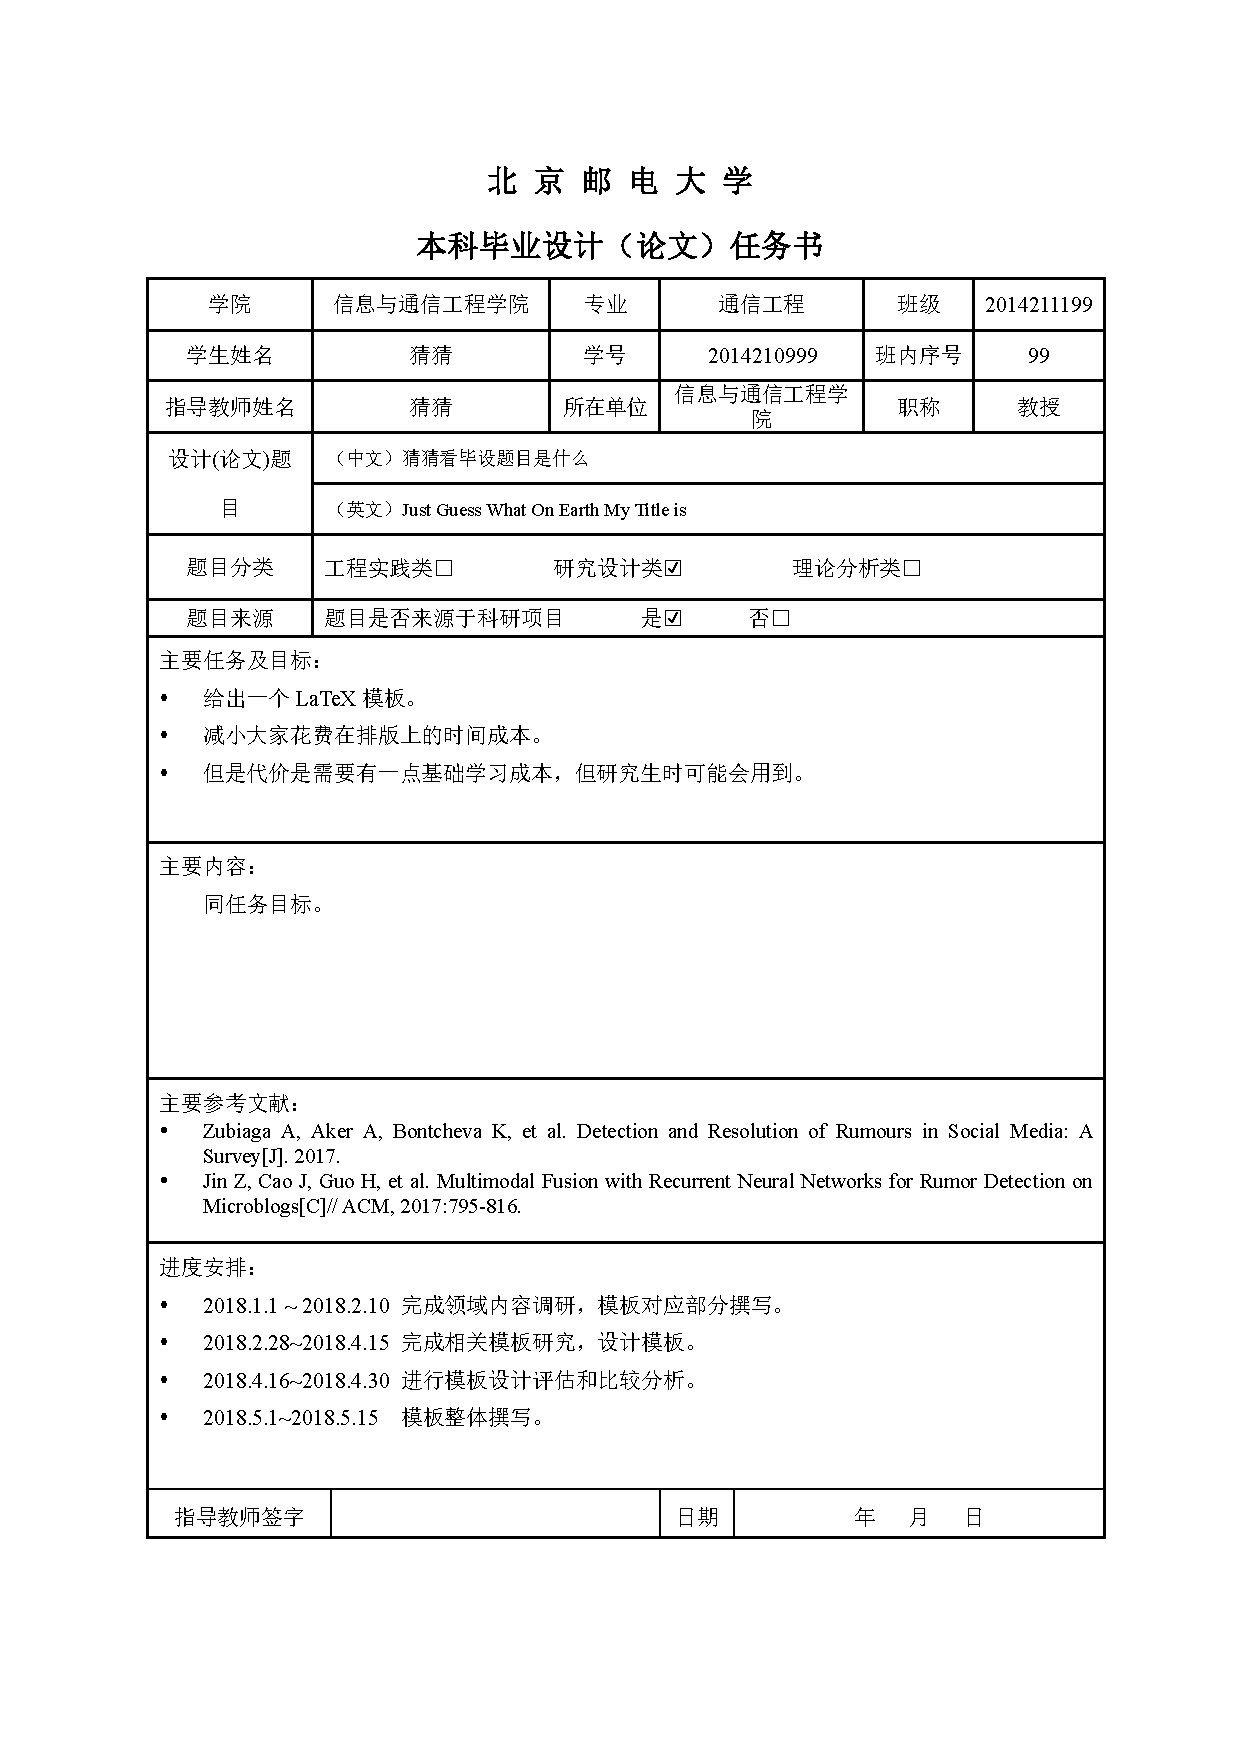
\includepdf[pages=-]{docs/task.pdf}  
\newpage

% 成绩评定表
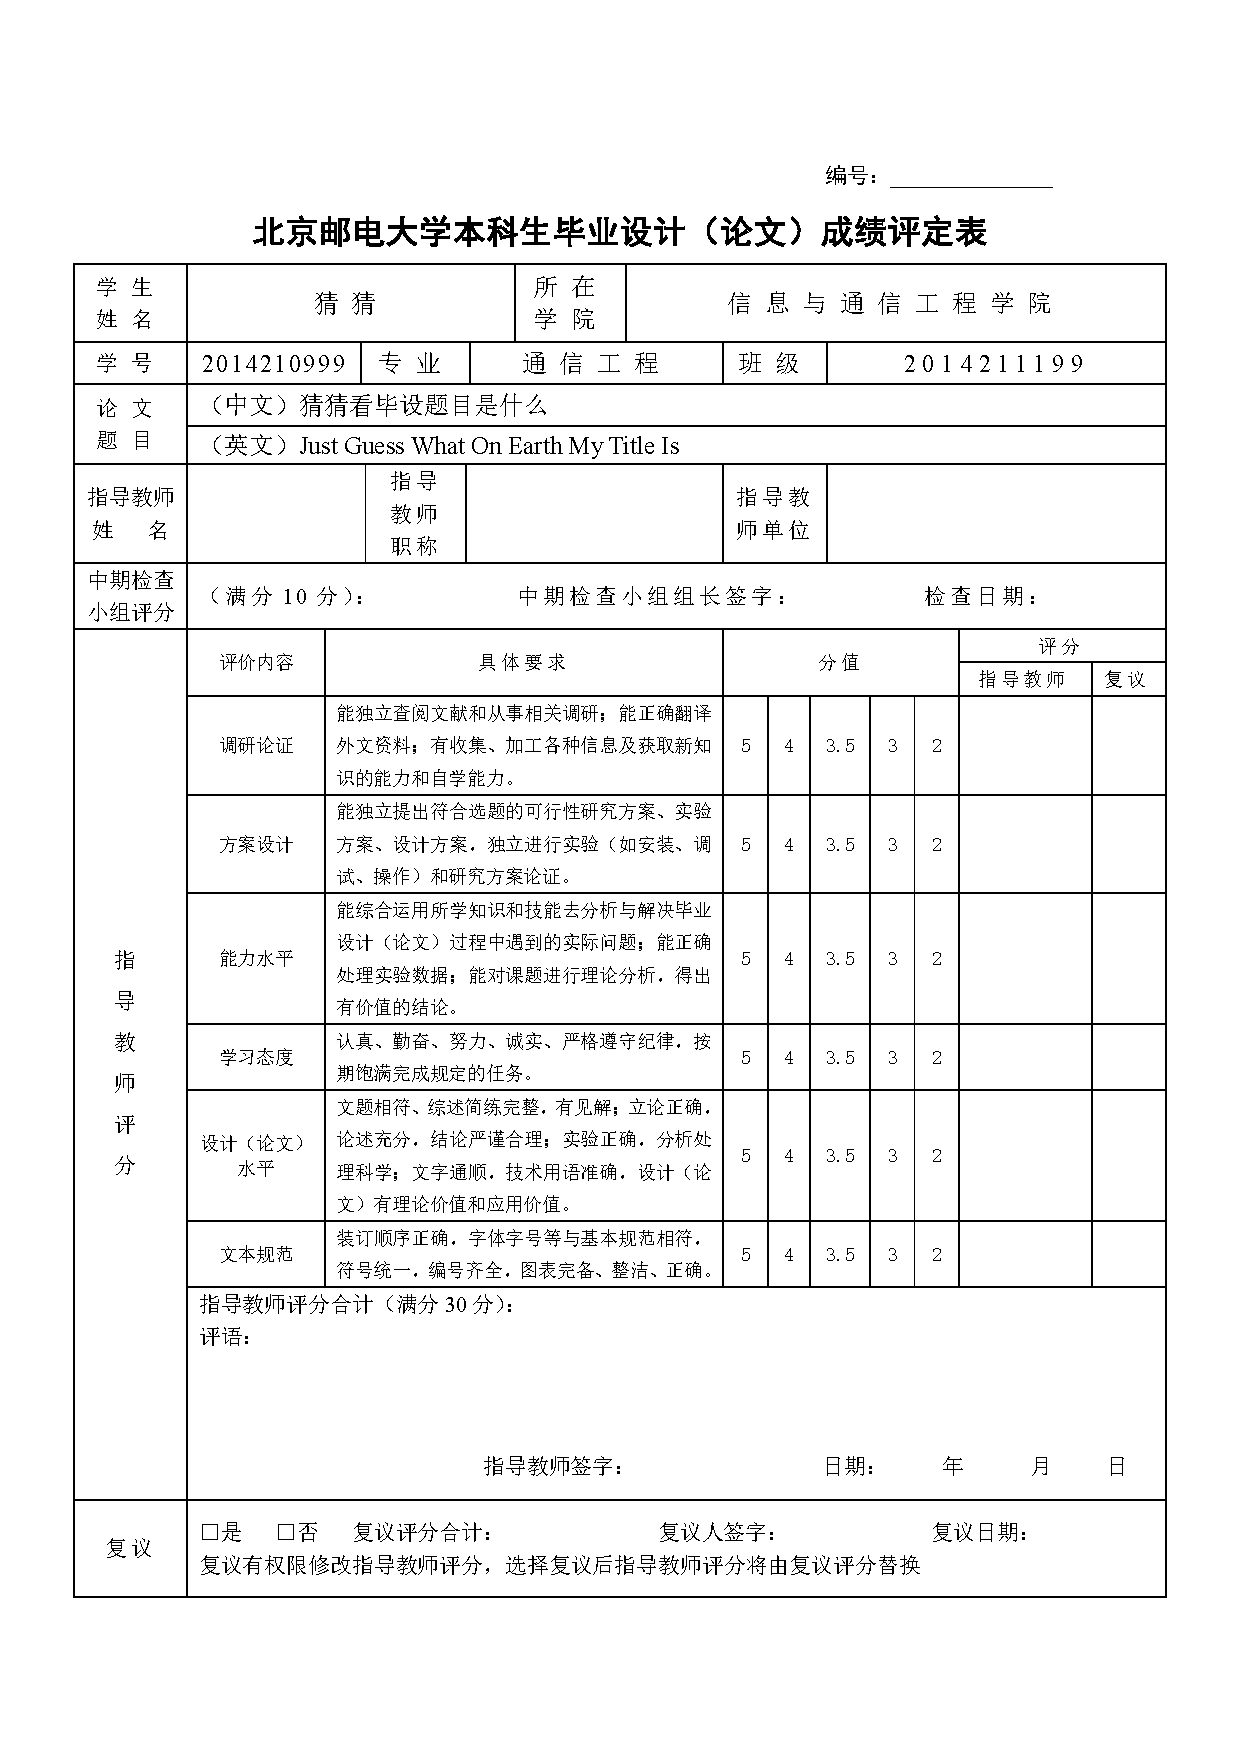
\includepdf[pages=-]{docs/scoreTable.pdf}  
\newpage

% 诚信声明

\includepdf[pages=-]{docs/statement.pdf} 
\newpage

%%%%%%%%%%%%%%%%%%%%%%%%%%%%%%%%%%%%%%%%%%%%%%%%%%%%%%%%%%%%%%%%%%%%
%                                                                  %
%   Copyright (c) 2010 - 2011 Caspar Zhang <casparant@gmail.com>   %
%                                                                  %
%   This copyrighted material is made available to anyone wishing  %
%   to use, modify, copy, or redistribute it subject to the terms  %
%   and conditions of the GNU General Public License version 2.    %
%                                                                  %
%   This program is distributed in the hope that it will be        %
%   useful, but WITHOUT ANY WARRANTY; without even the implied     %
%   warranty of MERCHANTABILITY or FITNESS FOR A PARTICULAR        %
%   PURPOSE. See the GNU General Public License for more details.  %
%                                                                  %
%   You should have received a copy of the GNU General Public      %
%   License along with this program; if not, write to the Free     %
%   Software Foundation, Inc., 51 Franklin Street, Fifth Floor,    %
%   Boston, MA 02110-1301, USA.                                    %
%                                                                  %
%%%%%%%%%%%%%%%%%%%%%%%%%%%%%%%%%%%%%%%%%%%%%%%%%%%%%%%%%%%%%%%%%%%%

% 你只需要修改下面几行就可以完成大部分内容的填写,
% 这要求你具有一定的LaTeX基础,但是如果你足够聪明,
% 不具有LaTeX基础也可以完成。

% 论文中文题目
\def\thesistitle{认知无线电系统组网研究}

% 论文英文题目
\def\thesistitleen{Research on cognitive radio adhoc networking technology}

% Thank Words
\def\thankwords{

此处请写致谢的内容。

它可以有多段。
}
    % Main items 
%%%%%%%%%%%%%%%%%%%%%%%%%%%%%%%%%%%%%%%%%%%%%%%%%%%%%%%%%%%%%%%%%%%%
%                                                                  %
%   Copyright (c) 2010 - 2011 Caspar Zhang <casparant@gmail.com>   %
%                                                                  %
%   This copyrighted material is made available to anyone wishing  %
%   to use, modify, copy, or redistribute it subject to the terms  %
%   and conditions of the GNU General Public License version 2.    %
%                                                                  %
%   This program is distributed in the hope that it will be        %
%   useful, but WITHOUT ANY WARRANTY; without even the implied     %
%   warranty of MERCHANTABILITY or FITNESS FOR A PARTICULAR        %
%   PURPOSE. See the GNU General Public License for more details.  %
%                                                                  %
%   You should have received a copy of the GNU General Public      %
%   License along with this program; if not, write to the Free     %
%   Software Foundation, Inc., 51 Franklin Street, Fifth Floor,    %
%   Boston, MA 02110-1301, USA.                                    %
%                                                                  %
%%%%%%%%%%%%%%%%%%%%%%%%%%%%%%%%%%%%%%%%%%%%%%%%%%%%%%%%%%%%%%%%%%%%

% 你只需要修改下面内容就可以完成中英文摘要,
% 这要求你具有一定的LaTeX基础,但是还是那句话,
% 如果你足够聪明,不具有LaTeX基础也可以完成。

% 中文摘要
\def\abstractcn{
%从这里开始写你的摘要,分段需要空一行。
  随着无线频谱资源的不断使用,为了满足人类社会对于通信的需求,认知无线电组网技术应运而生,
成为了缓解频谱压力的一大研究热点方向。传统的认知网络使用中心控制结构,依靠控制中心,
例如基站,基站可以辅助认知无线电设备发现临近的用户与接入节点,不断的更新邻近用户的信息,
在本地网中发送节点以无线自组网的方式建立与接收节点的通信路径,并能够能够通过基站建立与其它本地网接收节点的单点与多点通信。
但是这种方式受制于控制中心地理位置,不符合日后移动认知网络的需求,如果采用固定信道作为控制信道则会浪费大量频谱资源
这是与认知无线电的原则相违背的。
  
为了满足非固定式的认知自组网的建立需求,本文研究了与组网相关的以下内容:信道交汇,对授权用户与认知用户进行建模,实现环境感知与基于CGB算法的自动跳频完成相邻节点交汇;拓扑发现:研究了不同指标下的两种拓扑发现方法,给出了相关 协议与发现过程的代码仿真分析;
路由选择与数据传输:对于不同的组网要求给出了两种路由选择与传输的数据包类型,分析了各个模式下的网络性能。


%摘要结束
}

% 中文关键字 
% TODO: 改成可变长度的
\def\abscnkeyone{认知无线电}
\def\abscnkeytwo{自组网}
\def\abscnkeythree{拓扑发现}
\def\abscnkeyfour{路由协议}
\def\abscnkeyfive{}


% ABSTRACT
\def\abstracten{
%Your abstract here, to make a new paragraph, give an extra blank line please.
  With the continuous use of wireless spectrum resources,cognitive radio networking technology was born for human society's need for communication,and has become a hot research topic to relieve the spectrum pressure. 
Traditional cognitive networks use a central control structure,which depends on its control center like BS.BS can auxiliary cognitive radio equipments to find adjacent users and access nodes.
so that SUs can update information for adjacent users.In this network, the communication path of the receiving node is established by wireless ad-hoc network so the sending nodes can sstablish a single point or multi-point communication with other local network receiving nodes.
by the BS.But because of the location of the control center,this kind of network can't meet the needs of mobile cognitive networks in the future.And choosing a fixed channel as control channel
will waste a lot of spectrum resource,which is contrary to the principle of cognitive radio. 

 To meet the need of cognitive radio network,this paper studies the following contents related to network
 :Channel intersection, modling the activity of PUs and SUs,realization of the environment perception and the CGB algorithm based on 
 automatic frequency hopping to Realization of the environment perception and the CGB algorithm based on automatic frequency hopping to complete
 intersection with adjacent nodes .Topology discovery,two methods of topology discovery under different indexes are studied, and the code simulation analysis of relevant protocol and discovery process is given.
 Routing and data transmission,the data packet types of two kinds of routing and transmission are given for different network requirements, and the network performance under each mode is analyzed.


%Abstract done
}

% Key Words 
% TODO: 改成可变长度的
\def\absenkeyone{cognitive radio}
\def\absenkeytwo{adhoc networks}
\def\absenkeythree{topology discovery}
\def\absenkeyfour{routing protocol}
\def\absenkeyfive{}



  % Abstract
\frontmatter\tableofcontents % Content

% 正文
\newpage\mainmatter
\fancypagestyle{plain}{\pagestyle{fancy}} % Add head to new chapter
\pagestyle{fancy} % Head and foot
%\let\cleardoublepagebak=\cleardoublepage
%\let\cleardoublepage\relax % Make new chapter stay on old page

%%%%%%%%%%%%%%%%%%%%%%%%%%%%% Main Area %%%%%%%%%%%%%%%%%%%%%%%%%%%%

\chapter{绪论}
\section{选题背景及意义}
  无线电频谱是非再生资源并且是国家的战略资源,许多无线通信方式需要在政府划分的频带下工作,这些频段也被称为授权频段,但是随着无线通信技术的发展,以及也有像700Mhz的通信黄金频段分配给广电总局进行无线电视的建设,这种分配方式使用效率极为低下,不符合与时俱进的无线通信的需要。无线局域网,蓝牙,zigbee等技术应用更为广泛导致了在ISM频段上也十分拥挤,这使得频带的整体使用率并不高而且在不同频段使用效率十分不平衡,频谱资源和卫星轨位需求愈加旺盛,需求增长与频谱的静态分配带来的频谱稀缺问题日益浮现,规避拥堵的非授权频段,而在使用效率低下的授权频段内进行通信成为了解决这一问题的可行方案。

  认知无线电技术一经提出就被广泛讨论研究,认知无线电采用动态频谱分配策略(DSA),未授权用户或者辅助用户(SU)可以在授权频段内的自主寻找和使用未被授权用户(PU)占用的空闲的频谱资源,在时间和空间上同时增加频谱的使用效率。通过对周围环境的感知,调整自身工作最适当的频段与调制类型等参数,从而实现认知设备间的通信。

  认知无线电网络即认知设备间的网络,是一种多信道多节点无线网络,具有优秀的频谱复用性能与巨大的覆盖面积,拥有与传统无线通信网络不同的特点:认知无线电网络可以与普通无线通信网络共存并且不会产生干扰,其独特的认知功能可以智能分配无线资源,使得认知设备进行正常通信的同时不干扰授权频段内的其他系统的通信;系统支持多信道通信且不再具有传统网络的控制中心(例如基站),整个认知网络将会处于不同系统同时工作的嘈杂频谱背景中,这便要求网络不再使用统一固定的信道从而避免了盲节点的产生,而应该随着周围环境的改变做出适应性变化,来保证信道可用的基础上满足通信的QoS需求,同时由于网络中每个认知设备所处的环境并不完全一致,若是想要达到最佳的通信效果应当舍弃控制中心进行集中管理,而是采用分布式的管理方式来配合移动终端状态快速变化的特点,控制中心不再以实体形式存在,而是用控制中心频率进行节点间信息的交换,每个认知设备都将具有完备的认知通信功能,可以同时作为管理节点与通信节点,这是目前的民用移动无线网络所不具备的特点。
  
  得益于认知自组网优秀的认知能力,认知自组网在不同的频谱占用情况下都可以寻找到合适的通信频段,在多种系统同时工作的环境中,认知设备的认知能力可以自主选择信道并满足自身的QoS需求,并且可以节省人工配置通信参数的成本,对于在医院,商场等活动设备密度高的场所建设内网有着天然的优势,由于认知设备周期性进行频谱感知,使得整个认知网络具有优秀的重构性能,在当前信道由于主用户活动不再可用时不会发生长时间的链路断裂而是直接跳跃到其他信道进行通信,CR设备可以根据无线环境动态编程,可以重构工作频率、调制方式、发射功率和通信协议等重要参数。同时由于是分布式管理,网络结构不会因为管理节点的瘫痪而无法通信,这也使得认知网络的重构性能更为优秀。相比于传统通信网络,认知无线网络的多信道通信模式可以更好的适应当前的无线环境,并且可以满足某些特殊的通信需求,在军用、民用方向都有着不同的优势。

\section{面临的问题与研究内容}
  认知无线电原则上是为了提高频谱的利用率,不应该一直占用信道进行控制信息的传送。但是这也是大多交汇算法的形式,它需要协商某频率作为控制信道来让想要加入的用户可以直接在该信道上发布信息,这种方法要求我们必须使用某一个频带,而这与将会降低该频带上的频谱利用率,所以应当舍弃固定频率公共控制信道的想法,寻找一种不需要固定的公共控制信道就能完成网络配置的组网策略。

  组网并非是两个节点之间的连接,比如蓝牙之类的主从设备配对,而应该是多节点之间互相通信,虽然双节点之间的信道交汇已经有很多策略,但是多点的组网策略与拓扑发现仍然还是初步发展,应当在节点交汇的基础上完成网络的构建。组网过程很重要的就是拓扑发现,此过程决定了网络的连通性,这也会是后期的路由协议设计以及数据传输的基础,起到了而在拓扑发现的过程中也是会存在网络主用户的干扰,这将会对信道可用率产生很大的影响,因此这也是多点组网的难点所在。
 
 自组网不能再任何时候都进行主用户的检测同时维护整个网络拓扑,也不能在任何阶段都允许新节点的加入。虽然为了使得所有节点都 尽可能同时加入某一个网络,可以延长整个拓扑建立的时间(周期数),但是组网的一个重要指标便是组建网络的时间消耗,为了整个网络的快速建立应当减少每个阶段的耗时,这两者的要求便会产生矛盾,如何平衡两者之间的需求来达到最佳的认知自组网络的性能,也是需要解决的问题。

    论文的主要研究内容如下:
\begin{enumerate}[\indent (1)] %加入\indent即可
\item 认知节点与主用户节点建模
\item  研究节点交汇算法与拓扑发现
\item  给出了两种信道中传输数据类型与相应的路由模式,分析不同情况下网络性能
\end{enumerate}
\section{认知无线电自组网发展现状}
\subsection{认知无线电网络架构}
  所谓组网,是指多节点之间根据某一协议完成互相之间信息的传输,形成一个具有完备的路由功能的通信整体。不同的网络架构拥有不同的组网算法与功能,认知无线电的网络架构主要有两种:控制中心型网络架构,分布式网络架构。
  
  控制中心型网络架构即集中式网络架构,也是传统认知无线通信网络的典型架构,在这种架构中,如图所示,认知设备与主用户处于相邻环境中,也就是意味着会有管理主用户的中心控制器,此控制器可同时对于通信范围内的认知设备进行管理,所有认知设备可以不具有完备的认知网络组件功能,由中心控制器负责无限资源的管理,需要组网时每个认知设备向控制中心申请空闲频谱资源,从而可以不需要认知设备提前完成相邻节点之间的信道交汇,只需要从控制中心获取自身相关的传输参数就可以快速完成与其他节点的交汇,在此基础上就可以完成组网。此种网络架构的负载压力主要由中心控制器承担,所以中心控制器的认知性能与处理速度直接决定了整个认知网络的性能,整个网络性能将会受制于控制中心的地理位置,通信范围等通信指标,并不适合野外军事,医用的环境。

%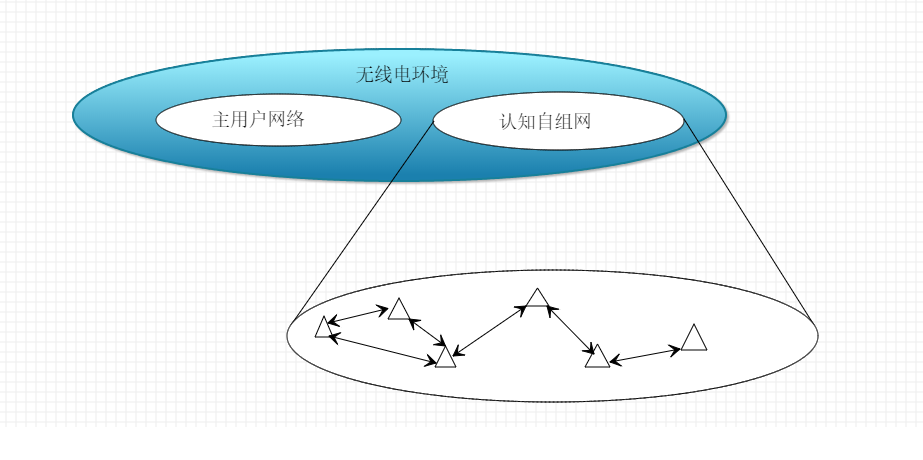
\includegraphics[width=5in]{C:/Users/menghui/Desktop/BUPTBachelorThesis-master/pictures/network.png}
\buptfigure{pictures/network}{分布式网络架构}{network}

  分布式网络架构,每个认知用户随机分布在不同位置,采用Ad Hoc模式,组成一个完整的认知网络。此种网络中每个认知设备地位平等,具有完备的认知自组网功能,同时负责路由器与终端的任务,每个终端自主学习周围环境并设计自身的通信参数。这种网络架构对于终端设备的要求提高,不过因为节点之间地位平等,不会因为某一个节点瘫痪造成整个网络的死亡,也正是由于分布式架构功能更为全面,整个组网过程的协议设计也相比更为困难。


  本文针对第二种网络架构进行研究,网络中每个节点都会具备认知自组网的所有功能组件,相比集中式网络架构将会更为稳健与可靠。

\subsection{感知学习过程}
  认知自组网系统的基础环节就是认知设备的感知学习过程,认知过程主要包括三个环节:频谱感知与分析, 频谱决策,频谱共享。
\begin{itemize}%项目符号
  \item 频谱感知与分析:认知设备需要扫描通信范围内的所有可用频段以及主用户占用的频段,分析空闲频段的可用概率,信道质量等信息。

  \item 频谱决策:认知设备应当根据需要的服务类型定制数据传输速率,传输方式以及使用频段,此过程保证了最佳的点对点通信质量。

  \item 频谱共享:多个认知用户接入时都会进行频谱感知与数据传输,多个认知用户之间应当避免同时占用一个频段,频谱共享可以使得多认知用户分享频谱资源而不产生互相之间的干扰。
 \end{itemize}
\subsection{节点交会过程}
  认知自组网是一个多信道网络,每个无线电设备都会检测到大量频谱空穴,在需要组网时,每个认知设备会与邻居节点产生一条信道进行信息的交换,而节点间同时在某一个信道相遇则被称为节点交会。
\subsection{拓扑发现过程}
  拓扑发现是在完成节点交汇的基础上获取整个网络结构的发现过程,网络研究界对捕获一个准确的网络拓扑结构图有极大兴趣,因为它有许多用途,是设计和评估新的协议以及服务的脆弱性分析是网络的基础。拓扑发现同样是认知自组网关键环节,是后续的路由设计的基础。
\subsection{路由发现与数据传输过程}
  认知自组网是多跳网络,在拓扑发现完成之后需要进行路由的发现以完成完备的网络通信功能,由于区别于普通的集中式无线网络,认知无线电的路由发现需要考虑能耗,跳频时延等问题,需要不同的策略来获得最佳的对认知设备适应性以及累积时延。
\section{认知自组网关键算法发展}
  
\subsection{频谱感知}
  频谱感知分为辅助频谱感知技术与独立频谱感知技术,辅助频谱感知技术不对认知设备自身做频谱感知要求,但是需要由中心管理设备检测可用频谱,认知设备得到授权之后即可以直接使用此频段进行交汇,但是由于辅助频谱感知技术属于集中式网络架构,不符合认知自组网理念,所以主要介绍独立频谱感知技术的发展状况。

  \begin{itemize}
\item  \textbf{主用户检测}:独立频谱感知技术中,每个CR用户通过不同的频谱检测机制检测主用户的活动,避开主用户的工作频段,目前主流的频谱感知算法都是基于主用户发射机的检测算法,其中包括:1)匹配滤波器算法 2)能量检测算法\cite{uapp} 3)特征检测算法\cite{pinpu} 4)广义似然比检测,以上的算法可以满足不同的实际需求,所需求的信息环境也不同,并且不会产生PU与SU之间的通信,不过在阴影衰落较为严重的情境下,检测效果不佳;协作检测算法:协作检测需要多台CR设备交换各自的感知结果,弥补了单个节点由于PU用户信号的阴影衰落而无法被检测从而CR设备在此频段通信会对PU产生干扰的缺点,算法融合本地的感知信息可以使SU获取更为全面的主用户信息,不过此算法需要中继完成转发功能,在CR设备位置变化较快的时候检测难度也会很大;干扰温度检测:FCC提出了一种干扰温度模型,并给出了干扰温度界,也就是PU用户所能忍受的干扰大小,不过实际中无法给出确切的干扰温度,在噪声与主用户行为同时存在的情况下(绝大部分室外环境)CR设备并无法分辨两者之间的区别,这也是该算法的缺点。
\item \textbf{合作频谱感知}:合作频谱感知技术并非辅助频谱感知,由于每个认知设备独立进行频谱感知不一定可以获得完整的频谱信息,所以基于合作感知的mac层协议不断被提出,合作频谱感知技术意为认知用户间以某种策略将独立得到的感知结果进行分析叠加,从而尽力获得全面准确的频谱感知结果,文献\cite{uaQQ}中提出了一种基于簇的能量采集的协同频谱感知,认知节点基于它们的接收功率水平聚集在一起,以提高感知性能,文献\cite{Peipei}提出的基于簇的协同频谱感知,在成簇的基础上,根据每个簇内成员的采集到的信道的方差信息优化自身的大小。文献\cite{hezuo}中提出了在簇成员发现某一个频谱不可用时,会立刻通过洪泛路由发送给簇内其他成员终止自身的信息传输。
\end{itemize}
\subsection{频谱决策}
  通过频谱感知获取到可用频带的信息后,如何根据需要的服务类型与服务质量选择最适合进行传输作业的信道,是认知自组网的重要研究内容之一,是接入控制与频谱分配的前提。
  非合作的本地频谱决策,最简单的方式是随机选择一个可用频谱,不对频谱的可用概率,链路质量等传输参数进行考虑,这样可以节省大量的算力,但是并不能保证通信质量。频谱决策应当考虑信道通信质量的同时考虑信道的数学统计特征,此特征根据主用户的动作进行实时改变,适合在主用户活动剧烈的条件下寻找适合的信道,这样可以尽量减少由于主用户的频繁改变导致的信道可用性差的问题,虽然一些频段的通信质量高,但是有可能主用户的活动同样强烈,这也会使得认知设备频繁执行跳频过程影响整个网络的性能,文献\cite{spectrumdecision}提出了基于信道主用户活动概率的频谱决策方案,在次用户负荷较低时选择可用概率最高的信道可以有效节约系统时间。
\subsection{频谱共享}
  在某个认知设备的通信范围内是可能存在多个认知设备的,在这种条件下,由于自私策略, 每个认知设备在感知到类似的频谱结果后,必然会优先使用某个最佳的信道,这会使得此信道由于认知设备的争夺而不再具有通信的可能性,如果这种条件下每个设备都可以与通信范围内的认知节点分享频谱感知结果,通过协商不再争夺同一个信道,这样可以有效提升信道的使用率与网络的性能,所以频谱分享对于认知设备密度高的场景十分有必要,目前的频谱共享依然分为集中式与分布式两种,文献\cite{uafs}对比了两种策略,表明了集中式分享策略虽然可以达到最优,但是分布式可以使用较少的能耗。
  为了平衡两者之间的优缺点,目前的经典的方法就是在成簇的基础上完成频谱共享,同时具有分布式与集中式的优势,当然也是对两者的一种妥协。
\subsection{频谱移动}
  认知设备在通信过程中使用的信道有可能会被主用户占用或者自身的移动导致某一个频带不再可用,此时认知设备必须中断数据的传输,这在射频设备的表现为频率的改变,在这个网络中表现为某个节点暂时丢失(时间很短),在多跳网络中,频谱切换会导致间歇性连通性,甚至是网络分区。在链路断裂之后进入其他信道重新进行组网或者重启数据传输过程,这个过程被称为频谱移动,频谱移动属于组网的基础技术,频谱移动对于射频物理层与链路层和网络层协议都提出了新的要求,所有通信层都应该保证在频谱切换的过程中对数据通信的影响最小,文献\cite{spectrumyidong}设计了集中式与分布式两种频谱切换与路由设计方案,其设计的互斥算法可以在路由迁移到新的链路上是不干扰其他链路同时降低整体链路迁移的时延。
  
  频谱切换带来的主要结果是数据传输的延时。频谱移动的主要原因来源于主用户的活动,所以制定最佳的频谱移动策略在于处理主用户的活动上,对主用户活动进行合理的建模,分析主用户的时间统计特性,从而保证频谱移动的次数尽量减少。
\subsection{路由协议}
  认知无线电网络是电池供电的,且相对密度较大,面对不同的应用程序,认知网络的QoS要求也不尽相同,文献\cite{luyou1}中提出使用基于簇的节点收缩的簇头选择方案与基于可用概率的路由选择方案,在这种簇头选举的条件下,路由选择具有最高可用性概率的路由,即途径路由信道可用概率的乘积。在文献\cite{luyou2}中提出了一种基于簇的路由协议,将簇分为簇头、成员节点、中继节点和网关节点这四类节点,此路由算法中,节点不需要开机后立刻确认频谱的使用情况,而是随着时间的推移不断确定信道可用性,一组地理相邻的认知设备倾向于共享相似的可用通道集,因此较小的集群规模会增加集群中公共通道的数量,算法中根据度大小,移动特征与可用信道数目确定簇头,之后由簇头广播RREQ消息维护整个网络的路由,该种方法使得路由协议的开销,吞吐量,延时都达到了最优。
\section{论文组织结构}
  论文一共包括四个章节,具体安排如下:
  第二章对主用户以及认知用户的行为进行了建模,给出了一种从节点间的信道交汇到路由发现的组网算法,第三章通过代码实现给出仿真结果,针对仿真结果进行了分析;第四章指出了论文中的缺点与未来应该研究改善的方向。
\chapter{认知自组网算法}
  分布式认知自组网算法分为三个部分:节点交会,拓扑发现与路由设计。节点交会是整个组网过程的基础,认知用户使用跳频策略完成邻居节点的交会,文中对节点交会过程的主用户,次用户行为进行了建模,并给出了基于CGB算法的算法仿真结果。拓扑发现则是根据分簇思想给出了发现过程,以及算法的仿真结果。路由协议针对网络最低时延与最长寿命分别进行了设计,给出了两者的仿真结果与对比分析。
\section{系统建模}
  主用户模型需要考虑主用户到达离开模型,占用的信道;次用户行为则包括通信范围内频谱感知避让主用户
  ,主用户与次用户在同一个信道中的模型如图\ref{huitu}所示
\buptfigure{pictures/huitu}{同一信道内模型}{huitu}
\subsection{主用户行为建模}
  在100$\times$100的空间随机分布一定数量的主用户,每个主用户占用一个频段,互相之间占用的信道不重叠,每个主用户服从到达率为$\lambda$离开率为$\mu$的泊松分布。
  \subsection{认知用户行为建模}
  在100$\times$100的空间内随机分布一定数量的认知用户,每个认知用户可以扫描自身通信范围内的主用户活动即主用户占用的频谱,并可以将可用频段信息存储在可用频段列表中,每个认知用户具有一个唯一的macid($1,2,3 ...n$)。
 \section{点对点节点交会算法}
  文中使用的是CGB交汇算法\cite{认知无线自组网中组网技术研究},CGB算法首先将空间中可用的$N$条信道分为多组,即$N$=$C_{GROUP}$$\times$$C_{NUMBER}$,信道如下式所示
  
\begin{equation}
C={
\left[
\begin{matrix}
C_{11} & C_{12} & C_{13}  &\cdots & C_{1C_{NUMBER}} \\
C_{21} & C_{22} & C_{23}  &\cdots & C_{2C_{NUMBER}} \\
\vdots & \vdots & \vdots  &\vdots &  \vdots \\
C_{C_{GROUP}1} & C_{C_{GROUP}2} & C_{C_{GROUP}3}  &\cdots & C_{C_{GROUP}C_{NUMBER}} 
\end{matrix}  
\right]}
\end{equation}
 
 
  每个认知用户都已概率$P_i$和1-$P_i$分别进入主跳频模式和从跳频模式,两种模式的跳频策略如下:
  \begin{itemize}
  \item \textbf{主跳频模式}
  
  主跳频模式中跳频序列周期性生成,每个周期包含$N$个时隙,为生成主跳频序列,首先需要在集合$C$中随机选取一个子信道集合$C_m$作为新的集合的第一个元素,生成一个经过循环移位的新的信道集合
$M^{’}_A$ =  \{$C_m$,$C_{m+1}$,$\cdots$,$C_{n-2}$,$C_{C_{GROUP}-1}$ \}
然后按照子信道集合的顺序,分别从每个子信道集合中抽取一个空闲信道$c^{(m)}_{i_m}$,构成一个序列集合:
\begin{equation}
 M_A = \{ c^{(m)}_{i_m},c^{(m+1)}_{i_{m+1}},\cdots,c^{(n-2)}_{i_{n-2}},c^{(n-1)}_{i_{n-1}} \}
 \end{equation}
 主跳频序列的$M^{’}_A$在$N$个周期中并不会发生改变,只是在大周期中不断改变$M_A$ 。主跳频序列产生后会出现长度为$C_{GROUP}$$\times$ $C_{NUMBER}$的序列,其中每个跳频元素将会重复$C_{NUMBER}$次,详细的实现方法如图\ref{duotiaopin}。
\buptfigure{pictures/duotiaopin}{主跳频算法}{duotiaopin}

   \item \textbf{从跳频模式}
   
   从跳频模式与主调频模式相似,首先需要在集合$C$中随机选取一个子信道集合$C_m$作为新的集合的第一个元素,生成一个经过循环移位的新的信道集合
$M^{’}_B$ =  \{$C_m$,$C_{m+1}$,$\cdots$,$C_{n-2}$,$C_{C_{GROUP}-1}$ \}
,但是并不要求两者的$C_m$相同,而且只需要进行一次随机数的选举,之后按照顺序将选中的子信道集合中的元素排列进跳频序列即可。跳频模式的算法流程如图\ref{duotiaopin}。

  \item \textbf{运行实例}
  
  
  下面介绍程序代码中的实例实现GROUP\_NUMBER=27,GROUP\_LENGTH=6,在此条件下举例说明运行过程,假设信道分组
\begin{equation}
\begin{aligned}
&C_1 = \{ 1,2,3,4,5,6 \} \\
&C_2 = \{7,8,9,10,11,12\}\\
&C_3 = \{ 13,14,15,16,17,18 \}\\
&\vdots 
\end{aligned}
   \end{equation}
   假设此时生成的主跳频序列
   \begin{equation}
 M_A = \{ 2,10,13,\cdots \}
 \end{equation}
 生成的次跳频序列
  \begin{equation}
 M_B = \{ 1,2,3,4,5,6,1,2,3,4,\cdots \}
 \end{equation}
 主跳频序列每隔27次进行一次跳频,从调频模式下则会每隔时隙进行一次跳频,代码实现中时隙为小循环,两种模式下的交会如图\ref{jiaohui}所示
 \buptfigure{pictures/jiaohui}{交汇过程}{jiaohui}
 当两个节点分别进入主跳频模式与从跳频模式,在节点时间同步的基础上,由于主跳频序列包括所有子信道集合中的一个频率,即$C_{GROUP}$个频率点,而从跳频序列会包含某一个子信道集合中的所有元素,即$C_{NUMBER}$个频率点,在同步的条件下,必然可以在N个时隙(小循环)中完成,在异步的条件下,则需要2N个时隙(小循环),因此CGB算法属于有界算法,其MTTR为2N,在代码实现时也选择设为2N个循环进行节点交会。
 \end{itemize}
 \section{拓扑发现过程}
 拓扑发现过程是节点完成通信范围内的节点交会过程之后进行的操作,为了保证每个节点都加入拓扑,需要让每个节点至少拥有一个邻居节点,所以程序运行时如果出现通信范围内没有邻居节点时,组网必然无法包含所有点数,所以所有节点会重新进行随机位置算法。此拓扑发现算法基于成簇的拓扑发现,由于纯分布式网络拓扑发现过程中每个节点都需要得到完备的拓扑信息才能确定网络位置,维护成本随着节点数目增多而增加,所以选用不完全分布式组网方法,选择成簇算法可以减少网络的维护开销,只需要簇头承担拓扑维护工作以及数据转发工作,减轻了网络带宽的消耗。每个簇包含簇头(根节点R),一层叶子节点(L),二层叶子节点(E),多层节点(F,G...),可连通的簇间会存在网关节点(N)。拓扑发现算法最终可以将在散落在$100\times 100$内一定数目的认知设备连接成图,形成多个簇组成的完整的拓扑,整个拓扑发现算法需要以底层节点交会为基础,所以下面将会分别介绍拓扑发现的几个过程。
 \subsection{用户初始化}
 用户初始化过程会对主用户以及认知设备设定地理位置,分配主用户占用的频带,清空用户的路由表,子节点,父节点,信道可用列表等数据。认知设备具有完备的频谱感知功能,可以完整的感知到通信范围内的主用户占用的频率同时建立自身的可用信道列表,列表格式如\ref{channel}:
\buptfigure{pictures/channel}{信道列表}{channel}
 列表使用vector二维向量进行保存,自向量首位存储信道频率,第二位存储累积可用概率,第三位存储当前可用情况,每次进行频谱感知都会得到当前使用频谱是否存在主用户或者次用户数据活动,并将可用信道结果写入信道列表中,如果出现所有信道都被占用,则需要等待一个检测周期不做组网动作,在此之后重新进行频谱感知。
  频谱感知在算法中使用的是简单的对于主用户能量检测算法,对每个信道进行检测,每次检测都会获取范围内的主用户的$get_exist$函数结果,,此时主用户将会根据到达离开模型给出存在结果返回给此函数,认知设备根据主用户占用的信道获得自身的可用信道列表,此算法要求每个节点每次进入拓扑发现循环都会执行一次。
 \subsection{节点交会}
 由于节点交会时拓扑发现的基础,所以拓扑发现过程需要与节点交会相连接,而且拓扑发现的性能会对节点交汇过程产生一定的要求。文中使用的节点交会算法基于CGB算法,代码实现过程如下:
 根据\ref{duotiaopin}为每个CR设备产生主跳频序列或者从跳频序列,每个认知节点都有相同的概率$P$和$1-P$进入两种跳频模式,在通信范围内的两个节点分别进入两种模式中,则会发生信道交汇,如果进入同一种模式则很大可能无法检测,成功交汇概率即选择不同模式的概率:$P_i=1-P^2-(1-P)^2$
,以跳频序列为基础,两个设备进入不同的跳频模式,主跳频用户进行如下操作:在所有的可用频段广播寻找帧,如果收到回复则成功在某一信道完成交会,此时设备会交换可用信道列表,并对比选择一条$S1_i$ $\times$ 0.5 +$S1_j$ $ \times $0.5 取值最大的频段作为通信信道,此时的频谱决策应当以最大连通的统计特征作为参考,同时此频段为了避免干扰将会被其他认知用户感知到正在活动,这样就完成了频谱共享与频谱决策工作;从跳频用户需要在所有的可用信道监听广播寻找帧,如果接收到主跳频用户活动则同样进行频谱共享与频谱决策。
  
  节点交会阶段的耗时决定了拓扑的完整性,由于并非是所有节点间都能恰好处于主跳频与从跳频同时存在的状态,所以一次的结果并不能代表正确结果,整个阶段应当进行循环检测以求尽力得到完整信息。
\subsection{成簇}
  本文使用的是成簇算法,为了确定簇的结构,需要为每个簇确定簇头以及簇内成员。在此处使用获得最大连通性的簇头的选举方法。
  
  在初始化阶段,每个节点的节点状态(R,L,E...)都将会被初始化为R,即簇头节点,不过子节点数目初始化为0。进入簇头的选举阶段后应当开始向邻居节点发送簇头选举帧,帧结构如下:
\buptfigure{pictures/cutouxuanju}{簇头选举帧}{cutouxuanju}
收到帧后每个认知用户i将会进行如下判断操作:
\begin{itemize}
\item {SU[i].rootsituation==SU[j].rootsituation=='R'}

两个根节点相遇,则需要对子节点数目进行判断:
\begin{itemize}
\item {SU[i].sonnode.size()<=SU[j].sonnode.size()}

节点i的子节点数目如果小于等于节点j的子节点数目,将i的节点状态设置为L叶子节点,i的子节点状态设置为E第二层叶子节点,重复执行以确定节点所位于的叶子层数,同时把i的父节点设置为j,j的节点状态依然保持R即根节点状态,节点i将节点j加入到自身的子节点列表中。
\item {SU[i].sonnode.size()>=SU[j].sonnode.size()}

节点i的子节点数目大于j的子节点数目,此时j的节点状态更换为L,j的子节点变为E,重复执行同上,j节点把i节点设置为父节点,同时节点i将会把j加入自身的子节点向量中。

\end{itemize}
\item {SU[i].rootsituation=='R'\&\& SU[j].rootsituation!='R'}
  
  根节点与非根节点相遇,节点i直接将j加入子节点,j的节点状态设置为L,并确定j的子节点的节点状态,j将i设置为父节点。
\item {SU[i].rootsituation!='R'}
  
  由于自身为非根节点,与其他非根节点相遇不做任何操作。
\end{itemize}
  此阶段结束后会产生不同的节点状态以及多个簇,此时由于在簇头选举过程中节点可能多次更换父节点,但是却不能确定是到达簇头的最短状态,而且此时并不存在网关节点N,所以需要进行其他过程来确定最短到簇头状态以及网关节点。当此状态结束后,所有的子节点逐级上传信道列表的信息,由簇头选择簇内通信应该使用的信道,所有的簇头节点需要进入主跳频模式发送寻找帧,如果此时新接入节点接收到寻找帧可以直接作为L状态进入下一过程,如果新接入节点在2N时隙之后依然没有接收到簇头的消息则作为R状态直接进入下一个过程。
  \subsection{最短拓扑发现}
  由于在成簇阶段的簇头选举过程不能获得最佳拓扑,所以需要在现成的簇的基础上选择节点的最佳状态。此过程需要所有的簇头节点向子节点列表中的所有子节点广播消息,帧格式如下:

\begin{table}[h]
  \setlength{\belowcaptionskip}{7pt}
  \centering
  \caption{广播帧}
  \begin{tabular}{|c|c|c|} 
  $su[ROOT].macid$&$su[Last].macid$&$T$\\
  广播节点macid&上一跳节点macid&跳数
  \end{tabular}
  \end{table}

  当节点i收到广播帧后,将会做如\ref{processdata}处理:
  
  \buptfigure{pictures/processdata}{处理广播消息帧}{processdata}
  每个节点都会产生一个层数值,与节点状态的对应关系为R->0, L->1....,接收到广播帧后,如果自身状态为簇头,则不做任何处理,如果帧中的跳数低于自身的层数T,说明有一条更短的到达其他簇头的路径,此时应当把该簇头作为自己记录的簇头节点并与之交换频谱消息,并将转发节点设置为父节点,如果收到两个簇头的消息,证明此节点与两个簇头相连,则节点状态修改为网关节点N,之后继续进行转发。
  
  此过程完成后整个拓扑发现过程就已经完成,此时网络中将会出现网关节点,网关节点负责两个簇之间的通信需求,簇头负责维护整个簇的信道状况,每个簇头节点将会周期性发送寻找帧,以便新加入节点可以直接加入网络,每层叶子节点周期性向簇头节点汇报可用信道消息,以便在一个主用户产生时候将所有簇内节点搬移到其他频段发送消息。
  发生拓扑断裂的情况分三种:
  \begin{itemize}
  \item 可用频率断裂。如果簇头节点在当前频段的通信断裂,但是其他簇内成员不会受到影响,依然可以在此频率内进行通信,此时可以直接选举新的簇头,为了通信的需求不能等待簇头的重新连接,而应该尽快建立新的簇完成通信;如果其它层节点出现断裂,则影响较小,由于在频谱共享阶段存储了邻居节点的可用信道,所以可以选择可用概率次大的频率点监听,如果子节点数目不为0,会在次大概率信道发送寻找帧,而其父节点检测到子节点消失会在次大频率内发送寻找帧,如果重连成功则可直接加入原来拓扑并重新选举簇内的通信频率,一段时间后无法重连则再次进入成簇阶段,初始化自身通信参数。
  \item 能量耗尽。簇头节点能量必然是最先耗尽的,这也会导致网络的平均寿命不长,这个问题将会在下一章进行讨论。叶子节点能量耗尽会直接退出拓扑,其子节点与父节点依然同可用频率断裂进行处理。
  \item 超过通信范围断裂。算法中由于认知节点初始化之后不会再次发生位置移动,所以这部分并未出现在代码中,提出的想法是即使超过通信范围,也应该尝试在次大频率内等待重连一段时间,如果重新进入了簇的通信范围那么可以直接加入,如果再也不回到原始簇范围,将会重新回归成簇阶段,在新的通范围内建立通信。
  \end{itemize}
  \section{路由算法}
  目前无线网络大多是由Ad Hoc路由算法发展而来,主要分为三类:按需路由协议,先验式路由协议,混合式路由协议,路由协议应该考虑的因素有公平性,时延,吞吐量,开销等。本文中的路由算法是在拓扑发现阶段已经完成的情况下进行的,路由设计的优先考虑因素应当是时延,对于时延,在认知无线电中应该考虑跳频时延,这在簇间通信中出现,所以在经过网关节点N的时候应当考虑跳频时延,其次则是地理位置所决定的节点距离产生的传输时延,对于处理时延,由于帧长一定,所以每个节点的处理时延大致相同,可以不予考虑。下面对于不用的网络需求给出了按需路由协议与先验路由协议的算法。
  \subsection{按需路由协议}
  按需路由协议,顾名思义是在节点需要进行通信的情况下申请路由通路,发起路由寻找协议,在寻找到路由协议之后进行数据传输,也仅仅在数据传输过程中进行路由的维护,在通信结束之后不再进行路由的发现与维护,按需路由协议DSR$\{Dynamic$ $ Source$ $ Routing\}$是最早应用按需路由协议的,所以文中使用的按需路由协议仿照DSR协议进行了设计。在这种方法中,每个节点都会维护自身的路由表,路由表中存储着到达不同节点的路由信息,路由表组织与实际运行结果如图\ref{luyoubiao}与\ref{luyoubiao1}所示。
   \buptfigure{pictures/luyoubiao}{路由表}{luyoubiao}
   \buptfigure{pictures/luyoubiao1}{路由表}{luyoubiao1}
   
  在节点需要通信时,会发起路由寻找,路由寻找帧的设计如下:
  \buptfigure{pictures/REQ}{路由寻找}{REQ}
  为了区别网络中传送的路由帧,需要对帧类型进行区分,路由寻找帧type=0。文中使用的路由属于洪泛式路由,当某个节点发起路由寻找的时候,将会向自身的子节点以及父节点发送此路由帧,节点收到路由帧之后将会进行如下处理:
  \begin{itemize}
  \item 当自身不为目的节点时,不会把路由写入自身的路由表,自身的macid写入到帧最后的路由表中,帧中的跳数加1,根据上一跳的地址增加传播时延,如果自身状态值为N,则需要增加跳频时延(50),根据上一跳中保存的地址,计算出距离加成,为了对信道的统计特征进行计算,应当在传输时延基础上乘以一个与信道可用概率相关的系数,这样可以表现出认知无线电中信道中间的区别,使用概率越高时延应当越小,所以文中取了$k\times\frac{1}{P}$。
  \item 当自身即为目的节点时,则会将收到的帧中的跳数,时延,源地址,路由消息录入自身的路由表中,同时向源节点按照最少跳数路由发送ACK帧,ACK帧只是在REQ帧的基础上增加了路由表的消息,在源节点收到该ACK消息后将会把路由消息进行处理后存入自身的路由表中。
  \end{itemize}
  由于网络的每个节点在数据传输过程中消耗的能量不同,所以传输过程中会出现节点死亡的状况,如果只保留最短路径的路由,很有可能在数据传输的过程中发生断裂,所以需要记录多条路由消息以尽力完成信息的传输。每次路由表的写入过程将会将此路由消息与当前路由表进行对比,如果产生重复将更新时延消息后不再重复写入。
  
  为了维护路由,在数据帧传送前需要对当前使用的路由进行能量统计,尽量少的收到其他节点回复的能量耗尽错误,此过程也是路由维护过程,在路由维护过程中将不会再次对路由通路的性能进行重新计算,只对最少能量节点的能量进行估计,估计可以连续传送的数据帧的数量。
  \subsection{先验路由协议}
  先验式路由协议需要每个节点都保存一张到达同一个网络中其他节点的路由消息表格,不同与按需路由,每当节点需要发送数据包的时候只需要直接在路由表查找现成的路由即可。在文中的实现方案是每隔一个周期进行一次查找作为路由维护过程,而不考虑是否需要进行通信,在需要通信的时候直接发送数据帧,不再执行路由发现过程。
  
  两种路由协议使用的路由发现帧与ACK帧相同,很明显两者对应的业务不同,路由协议的开销也不同,下一章节则对两者的不同环境下的性能进行了仿真分析。
  \section{数据传送}
  数据发送是在路由建立成功的基础上进行的,数据传送的性能主要考虑的因素就是收发时延,在不考虑网络寿命的条件下, 所有节点都应使用最小时延的信道进行数据的传输,这样可以获得最好的效果。但是网络的容量有限,所有数据包都使用最短路由,必将会使得路径的节点带宽占用率过高,不利于网络的维护与延长网络的寿命,所以对于不同的业务类型,应当进行不同的处理,文中主要是对于最低时延数据包和最长网络寿命对数据包的路由选择进行了选择。
  每种数据包的帧构造相同,构造如下\ref{data1}:
  \buptfigure{pictures/data1}{数据帧结构}{data1}
  
  数据包分为以下两种:
  \begin{itemize}
  \item 对时延要求高的业务,对应的type=1。在路由选择时应当选择最短时延路径,只需要在当前路由表中对比所有到达目的节点的路由,寻找到其中时延最短的节点,不考虑其能量的剩余,路径上的节点收到该数据包的时候,如果自身能量不足以进行下一步转发,则会沿着路径回馈能量不足以转发消息的错误,源节点接收到之后会在路由表中删除当前最短时延通路,之后重新执行最小时延路由选择,重复进行发送,由于路由维护只能估计可以发送数据包的数量,所以如果当前的路由都不再具有转发条件,就会重新寻找路由。
  \item 对时延要求低的业务,其type=2。此类型的业务对于时延要求不高,可以不再按照最低时延方案进行寻找,而可以为了获得最长的网络寿命,尽力不耗尽路由上某个节点的能量,所有路由的死亡时间尽量相同。在进行路由选择前,会沿着所有路由向目的节点发送一条能量查询帧,获取每个节点的能量并写入能量路由表的对应位置,此过程收集完一条可用路径的全部节点能量信息后,如果该条路由支持数据传送,就会直接按照此条通路进行一次数据通信,当所有的节点信息统计结束后,会把路由表中的每个路由条目中节点最低的节点作为该条路由的能量,在进行路由选择的时候,直接对比路由条目的能量,选取其中的最大者进行数据传输。路由表某个条目最低能量为1的时候,说明该条路由表不再可用,舍弃该条路由表。
  \end{itemize}
\chapter{仿真结果分析}
  仿真过程中,对于未给出的参量都是用默认的值
  \begin{table}[h]
  \setlength{\belowcaptionskip}{7pt}
  \centering
  \caption{默认参数}
 
  \begin{tabular}{cc} 
  认知用户数目&70\\
  主用户数目&55\\
  通信半径&35\\
  离开到达率&0.2\\
  时延系数&1\\
  最大跳数&5
  \end{tabular}
  \end{table}
  \section{组网时间}
   组网时间主要由节点交会,成簇阶段用时有关,节点交会过程中,每次进入主跳频模式和从跳频模式都会进行2N个循环,而可用信道的变化,也会直接导致认知设备在跳频模式中的交会时间,所以通信半径,主用户数目,主用户到达离开频率,认知设备数目都会对拓扑组网时间产生影响,所以下面分别对三种变量进行了仿真,分析了平均组网时间(CGB循环执行次数)。
  \subsection{通信半径的影响}
  图\ref{data-1R}中给出了通信半径对组网时间的影响,由于半径的增加,每个认知节点将会监测更多的主用户活动引起可用频段的减少,同时需要进行交汇的节点数也会增多,这会直接导致交会时间的延长,所以整个组网的时间也会延长,根据仿真也可以确定,随着通信半径的增加,组网时间将会不断延长。
   \begin{figure}[htbp]
\centering %使插入的图片居中显示
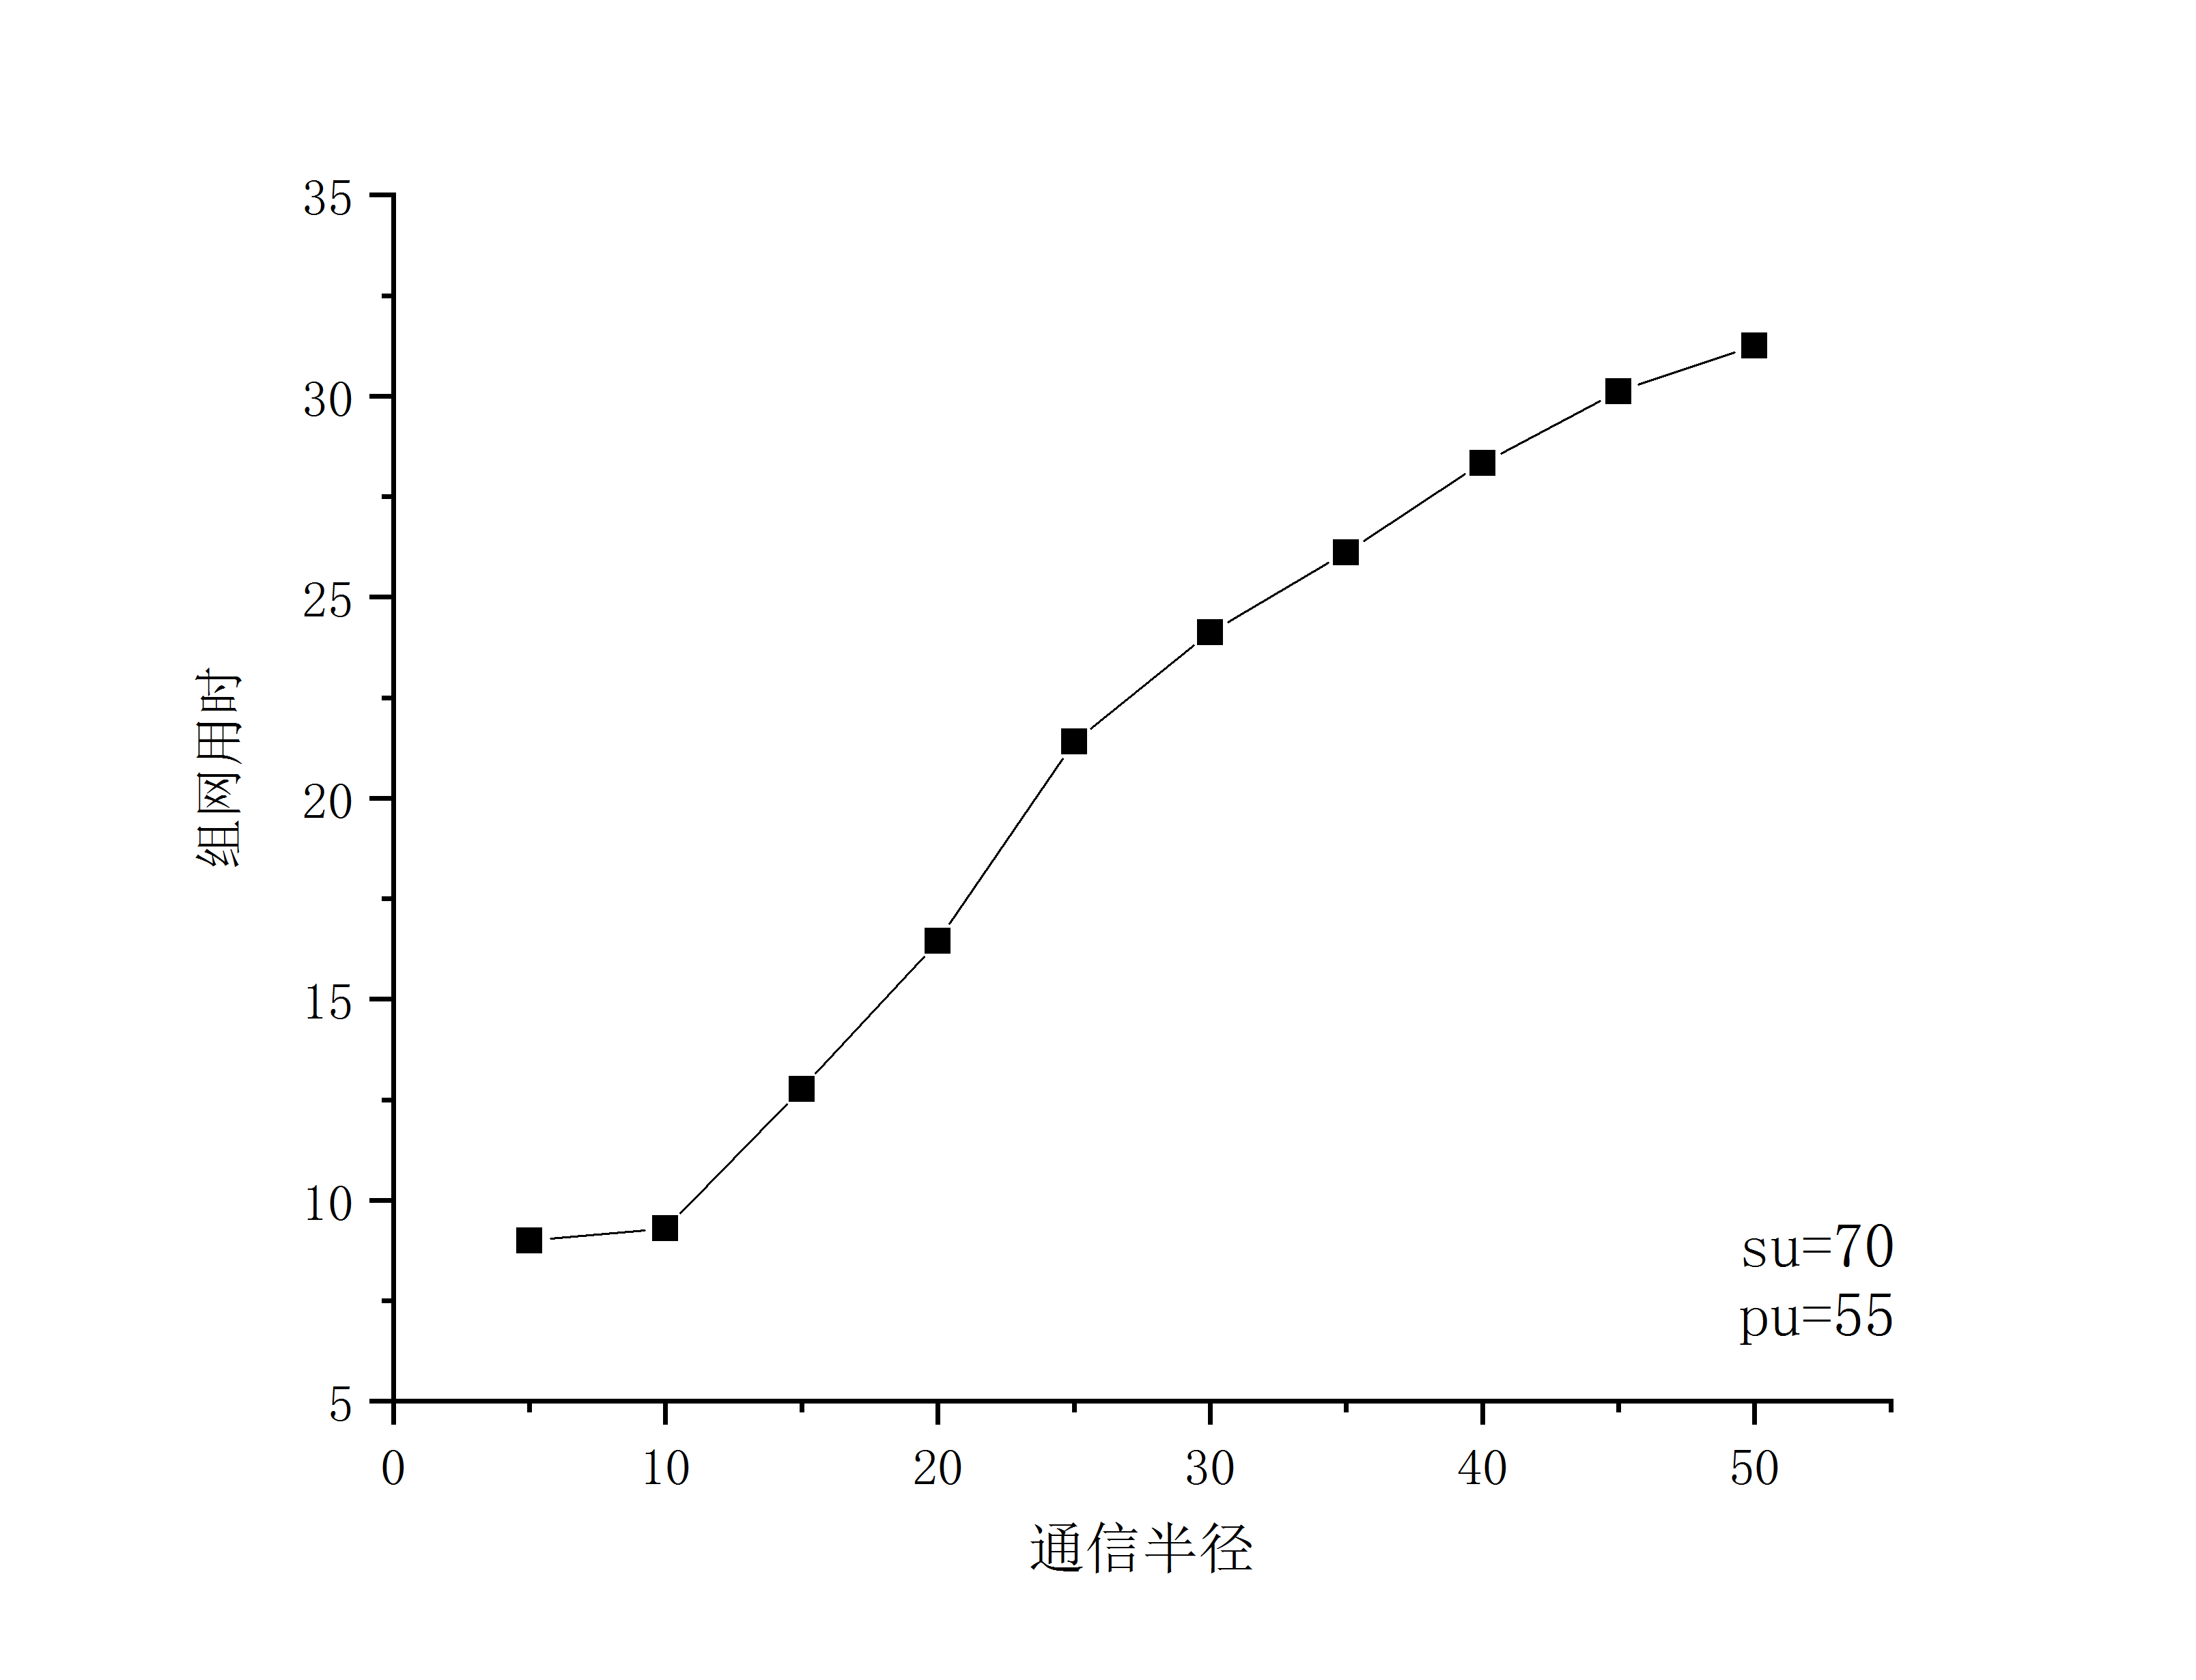
\includegraphics[scale=0.3]{pictures/data-1R.png} 
\caption{通信半径对组网时间的影响 } %插入图片的标题,一般放在图片的下方,放在表格的上方
\label{data-1R}
\end{figure}
 
  \subsection{认知设备数目与主用户数目的影响}
  认知设备数目的增加会直接引起节点密度的增加,在通信范围一定的情况下每个认知设备将会与更多的节点进行交会,分析如上,主要受到影响的依然是在节点交会阶段的耗时。主用户的影响主要体现在对频率的占用情况上,由于每个主用户都会占用一个不同的频段,这直接会导致认知设备可用信道的减少,当主用户节点数目占据了所有的信道分组之后所有节点都会无法进行通信,组网时间将无限延长。图中所示即为认知设备与主用户数目对于组网时间的影响,图中可知,认知设备与主用户数目的增多,的确会增加组网消耗的时间。
  \begin{figure}[htbp]
\centering %使插入的图片居中显示
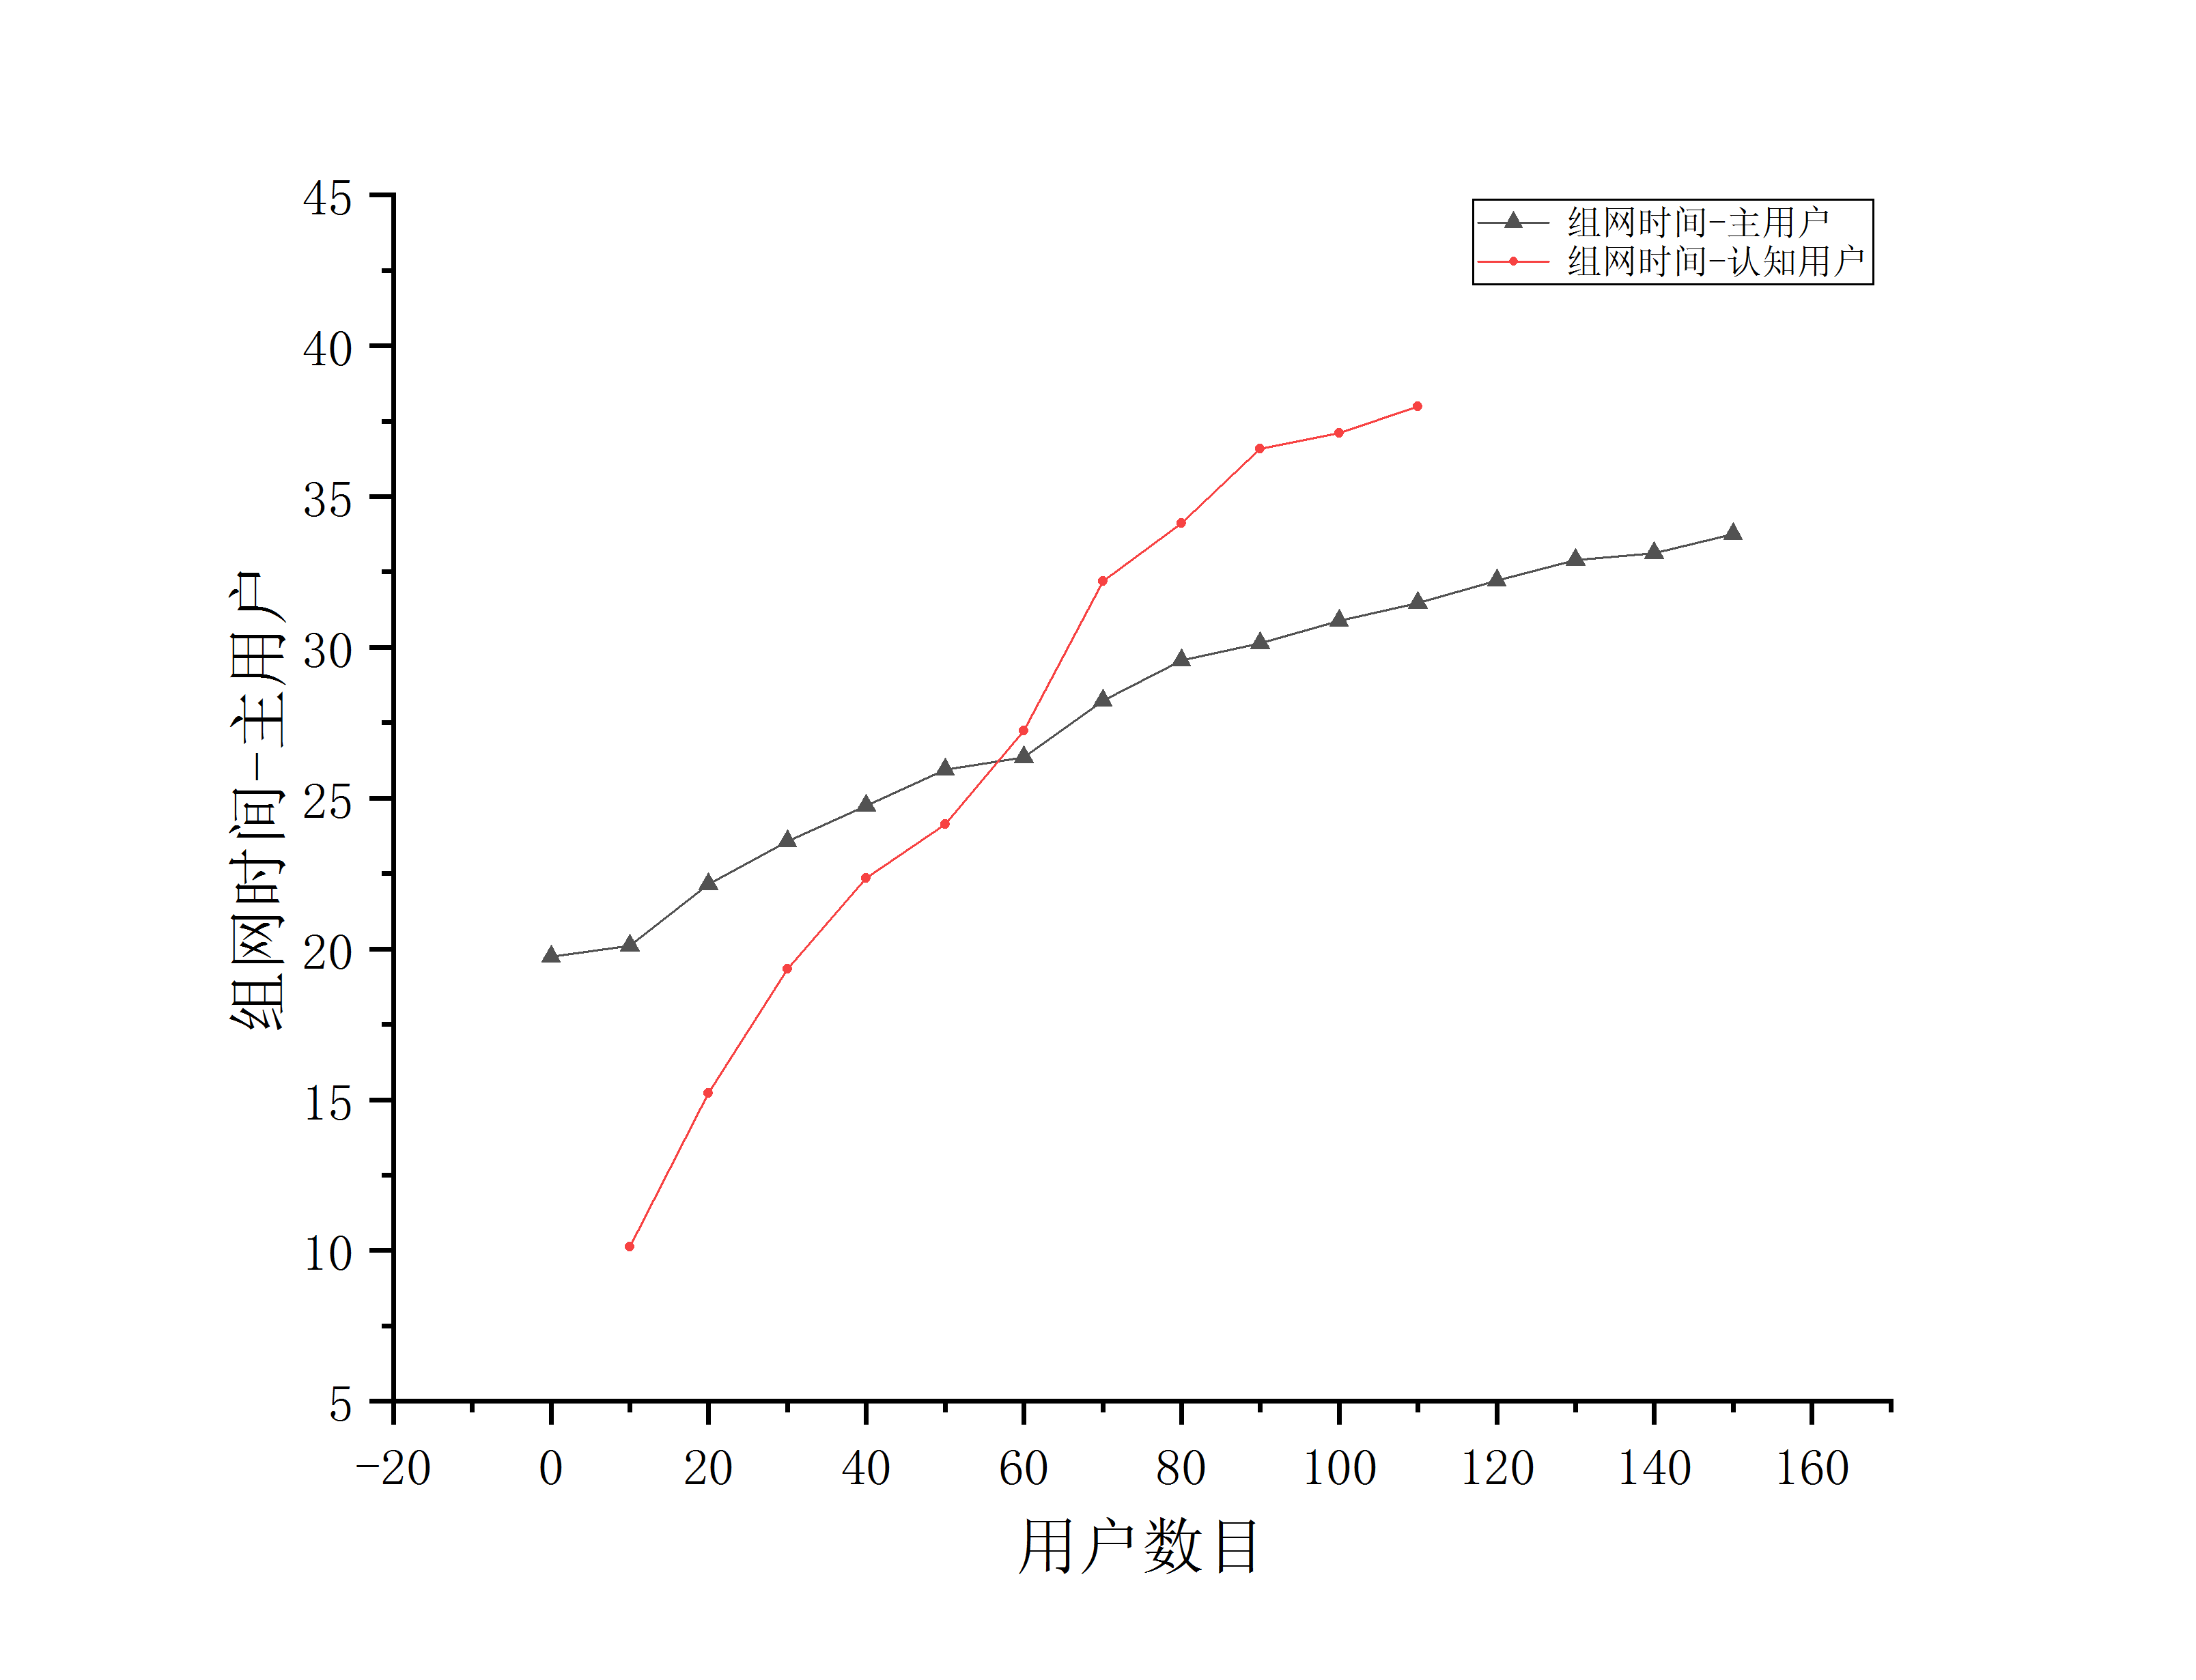
\includegraphics[scale=0.3]{pictures/PU-times.png} 
\caption{用户数目对组网时间的影响 } %插入图片的标题,一般放在图片的下方,放在表格的上方
\label{PUANDSU}
\end{figure}
  
  \subsection{主用户变化概率的影响}
  
  \begin{figure}[htbp]
\centering %使插入的图片居中显示
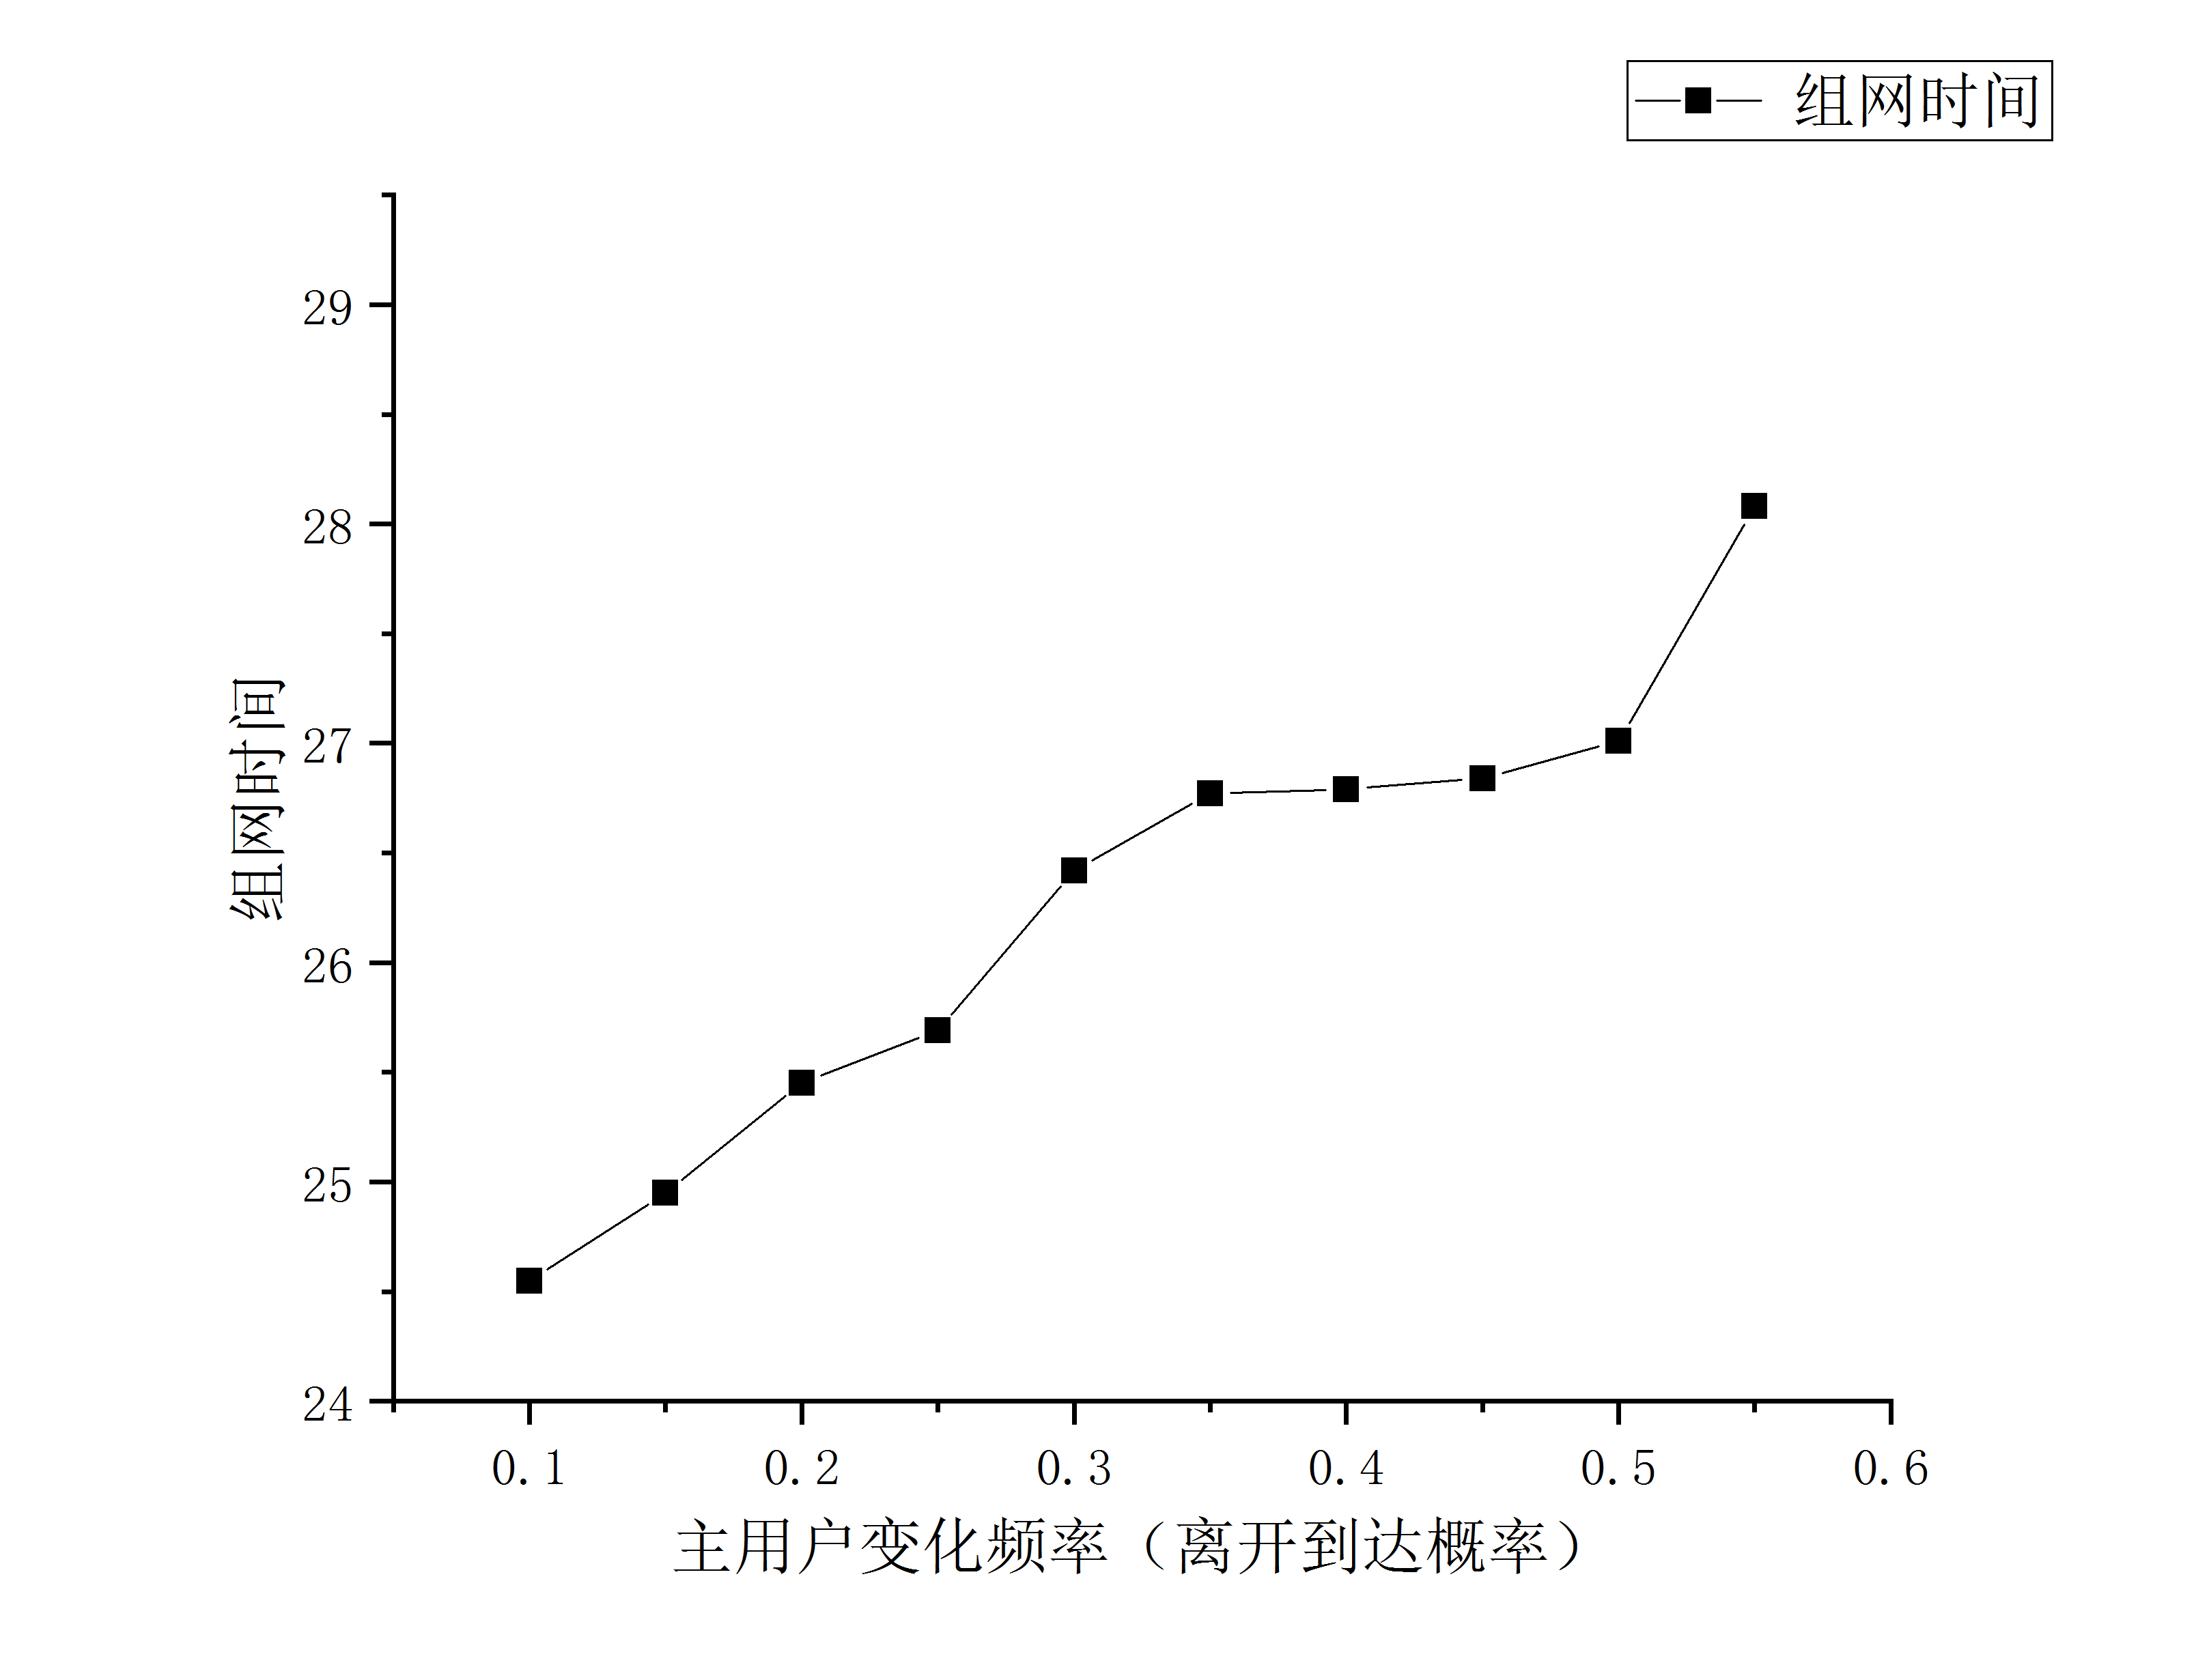
\includegraphics[scale=0.3]{pictures/PU-time.png} 
\caption{主用户变化概率对组网时间的影响 } %插入图片的标题,一般放在图片的下方,放在表格的上方
\label{PU-time}
\end{figure}
在仿真中,每个主用户都是具有到达离开模型的,而其中的到达率与离开率直接决定了主用户变化的频率,如果主用户一直不变化,那么认知设备可以更好地在稳定的可用信道上完成交汇,而随着主用户变化频率的增多,必将使得信道的可用概率变化更为突出,这也会延长组网时间,其仿真结果如图所示,根据图\ref{PU-time}中所示我们可以发现,在主用户变化频率低的时候,组网消耗的时间很短,而随着变化频率的增加,信道可用性变差,也使得组网时间不断延长。


  \section{组网成功率}
  根据数据结构课程内容可知,一个无向图的连通性可以利用它的邻接矩阵特性进行评定,我们在代码实现过程中,建立所有节点的邻接矩阵,根据自身的子节点向量与父节点,建立矩阵L:
  \begin{equation}
  L[i][j]= L[j][i] =
\left\{  
             \begin{array}{lr}  
             1 &if (SU[i].fathernode==SU[j] or SU[j]\in SU[i].sonnode)  \\  
       
             0 &else
             \end{array}  
\right.  
\end{equation}
  要判断一个无向图是否是连通图,可以对图做深度遍历(DFS)\cite{shujujiegou},遍历即从图的某个初始节点开始,对图中的每个节点进行访问,每个节点访问且仅访问一次。
  深度遍历步骤如下:
  \begin{itemize}
  \item 指定某个节点作为初始节点
  \item 若当前的访问节点的某个邻接节点未被访问,则开始对其深度遍历,若邻接节点都被访问则退回最近访问的节点,直到所有节点都被访问
  \item 若某个节点未被访问,重新选择某个节点进行深度遍历。
  \end{itemize}
  其伪代码如下
  \begin{lstlisting}
  count=0
  for 0 to CR_NUMBER
   for 0 to CR_NUMBER
   if L[i][j]&&!known(j)
   known[j]=1
   DFS(j)
   count++
\end{lstlisting}
  如果节点密度不一致,不同区域分布的节点数相差较大,如果通信半径较小,则会产生不相交的簇,簇之间不拥有任何网关节点,因此簇之间不再具有通信的可能性,而解决这个问题的首要办法就是平均节点的分布或者提高网络的通信半径,理论上通信半径越高,可以获得的节点消息越完整,越不容易出现孤立的节点或簇。图\ref{routing_1R}给出了通信半径对组网成功率的影响(由于在R<15时多次出现节点无邻居的情况,成功率很低,所以从15开始进行对比),图中可知上述理论是正确的,随着通信半径的提高,出现孤立节点的次数减少,更容易获得连通图,但是在通信半径高于35以后,成功率将会出现些许的下降,这是因为随着通信半径的增加,成簇的数目将会减少,而每个通信簇内的节点数目将会增多,所以平均到每个簇内会有更多的主用户占用信道,组网成功率就会有所下降。
 % \buptfigure{pictures/R-successp}{通信半径对组网成功率的影响}{R-successp}
  \begin{figure}[htbp]
\centering %使插入的图片居中显示
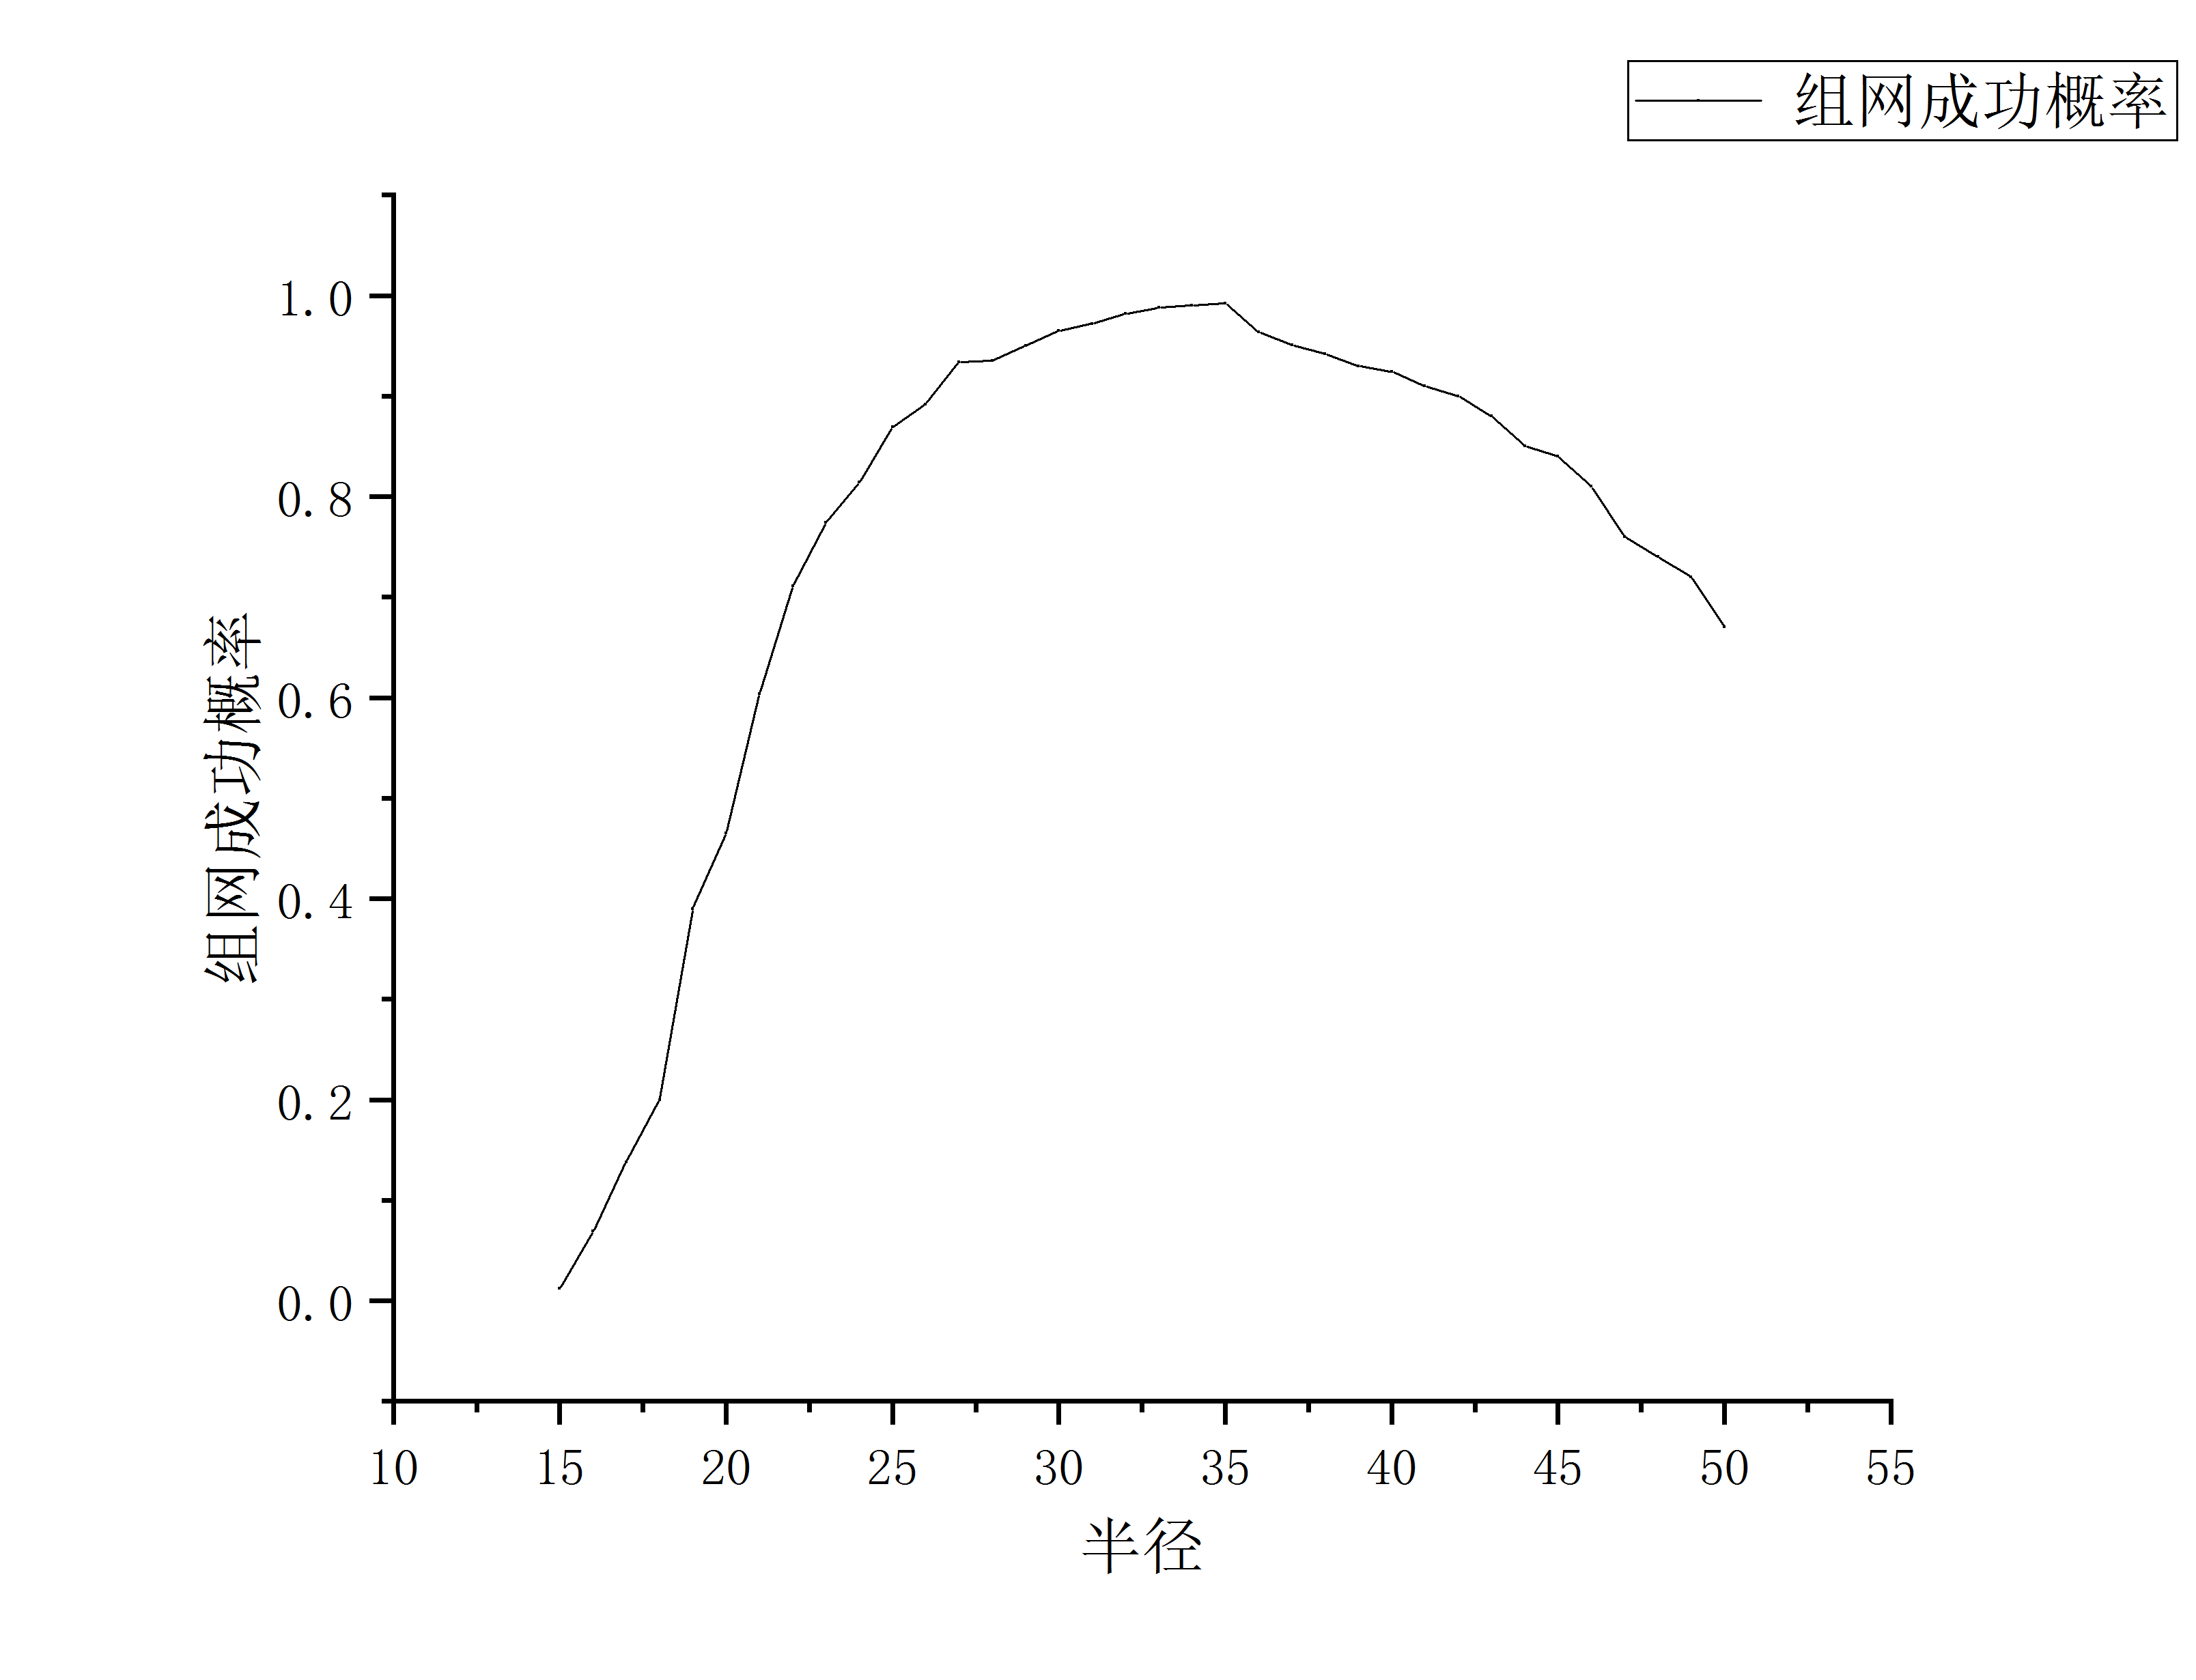
\includegraphics[scale=0.3]{pictures/R-successp.png} 
\caption{通信半径对组网成功率的影响} %插入图片的标题,一般放在图片的下方,放在表格的上方
\label{R-successp}
\end{figure}
  
  认知节点数目决定了整个范围内部的整体密度水平,也就是在通信范围不变的情况下也会影响组网成功率,认知节点数目越多,通信范围内可以连通的点越多,越不容易得到孤立的簇或者节点,认知节点数目过多的时候,会使得每个簇占用的空间区域较大,可以使用的信道数目变少,使得节点交会变得困难,所以组网成功率会不断下降,图\ref{CRPU-SUCCESS}给出了不同的节点数目对于组网成功率的影响。
   %\buptfigure{pictures/CRPU-SUCCESS}{节点数目对组网成功率的影响}{CRPU-SUCCESS}
    \begin{figure}[htbp]
\centering %使插入的图片居中显示
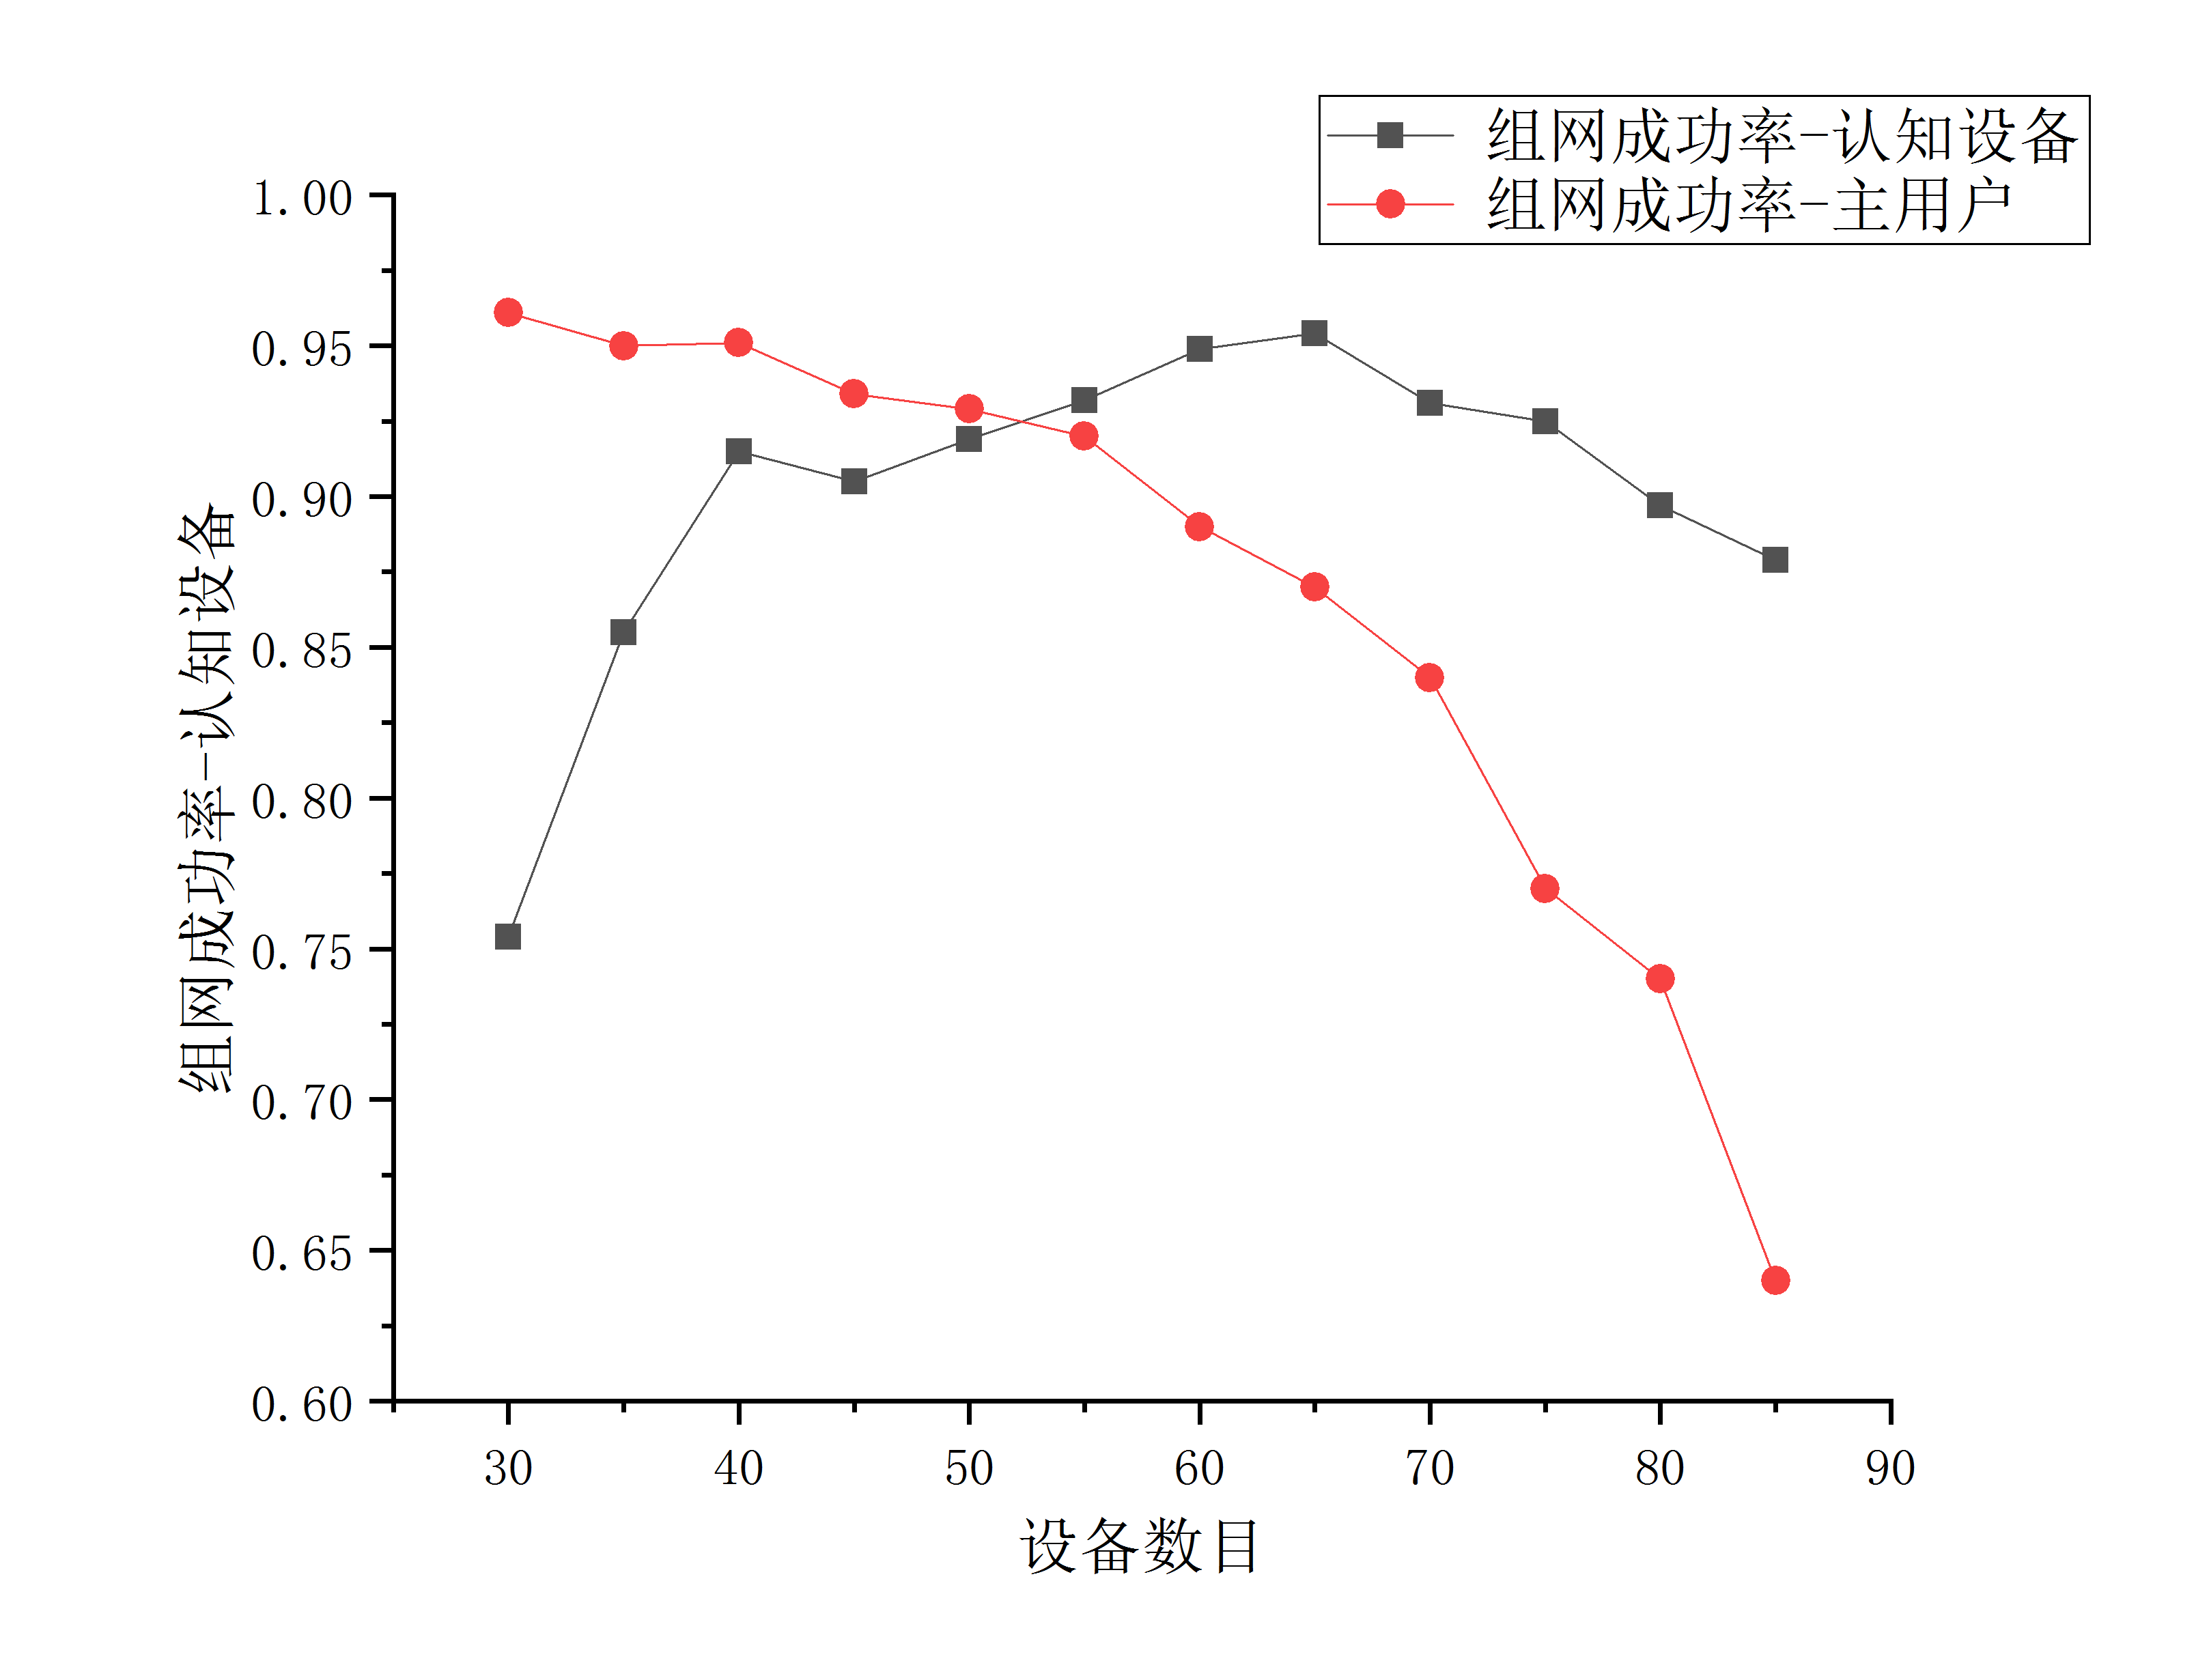
\includegraphics[scale=0.3]{pictures/CRPU-SUCCESS.png} 
\caption{节点数目对组网成功率的影响} %插入图片的标题,一般放在图片的下方,放在表格的上方
\label{CRPU-SUCCESS}
\end{figure}
  \section{网络健壮性}
  评价网络的好坏不仅仅只有连通性,还有网络的健壮性,当节点间的通路越多的时候,整个网络的连通性越强,根据图论的知识,可以根据一个图的$Laplacian$矩阵的次小特征值判断图的连通性,$Laplacian$矩阵特征值的性质:最小特征值为0,特征值中0的个数即连通子图的个数,第二特征值越大,代数连通度越高,图的健壮性越好,代码实现过程中参考了QR分解法求解特征值$Matrix_EigenValue$。$Laplacian$矩阵的定义为$L=D-W$,$W$为上述的邻接矩阵,$D$为度矩阵,度矩阵即
   \begin{equation}
  D[i][j]=
\left\{  
             \begin{array}{lr}  
             
           \displaystyle { \sum_{m=0}^{CR_{Number}-1}} W[m][j] &if(i==j)\\  
             -1 &else
             \end{array}  
\right.  
\end{equation}
  文中的认知网络由分簇的模型构成,不同簇之间可能拥有不同数目的网关节点,每个簇之间的网关节点越多,簇内的叶子层数越少,整个网络的健壮性越高,图\ref{pusu-strong}中给出了不同认知数目与主用户数目下对网络健壮性的影响以及通信半径(\ref{R-STRONG})对网络健壮性的影响。
   \begin{figure}[htbp]
\centering %使插入的图片居中显示
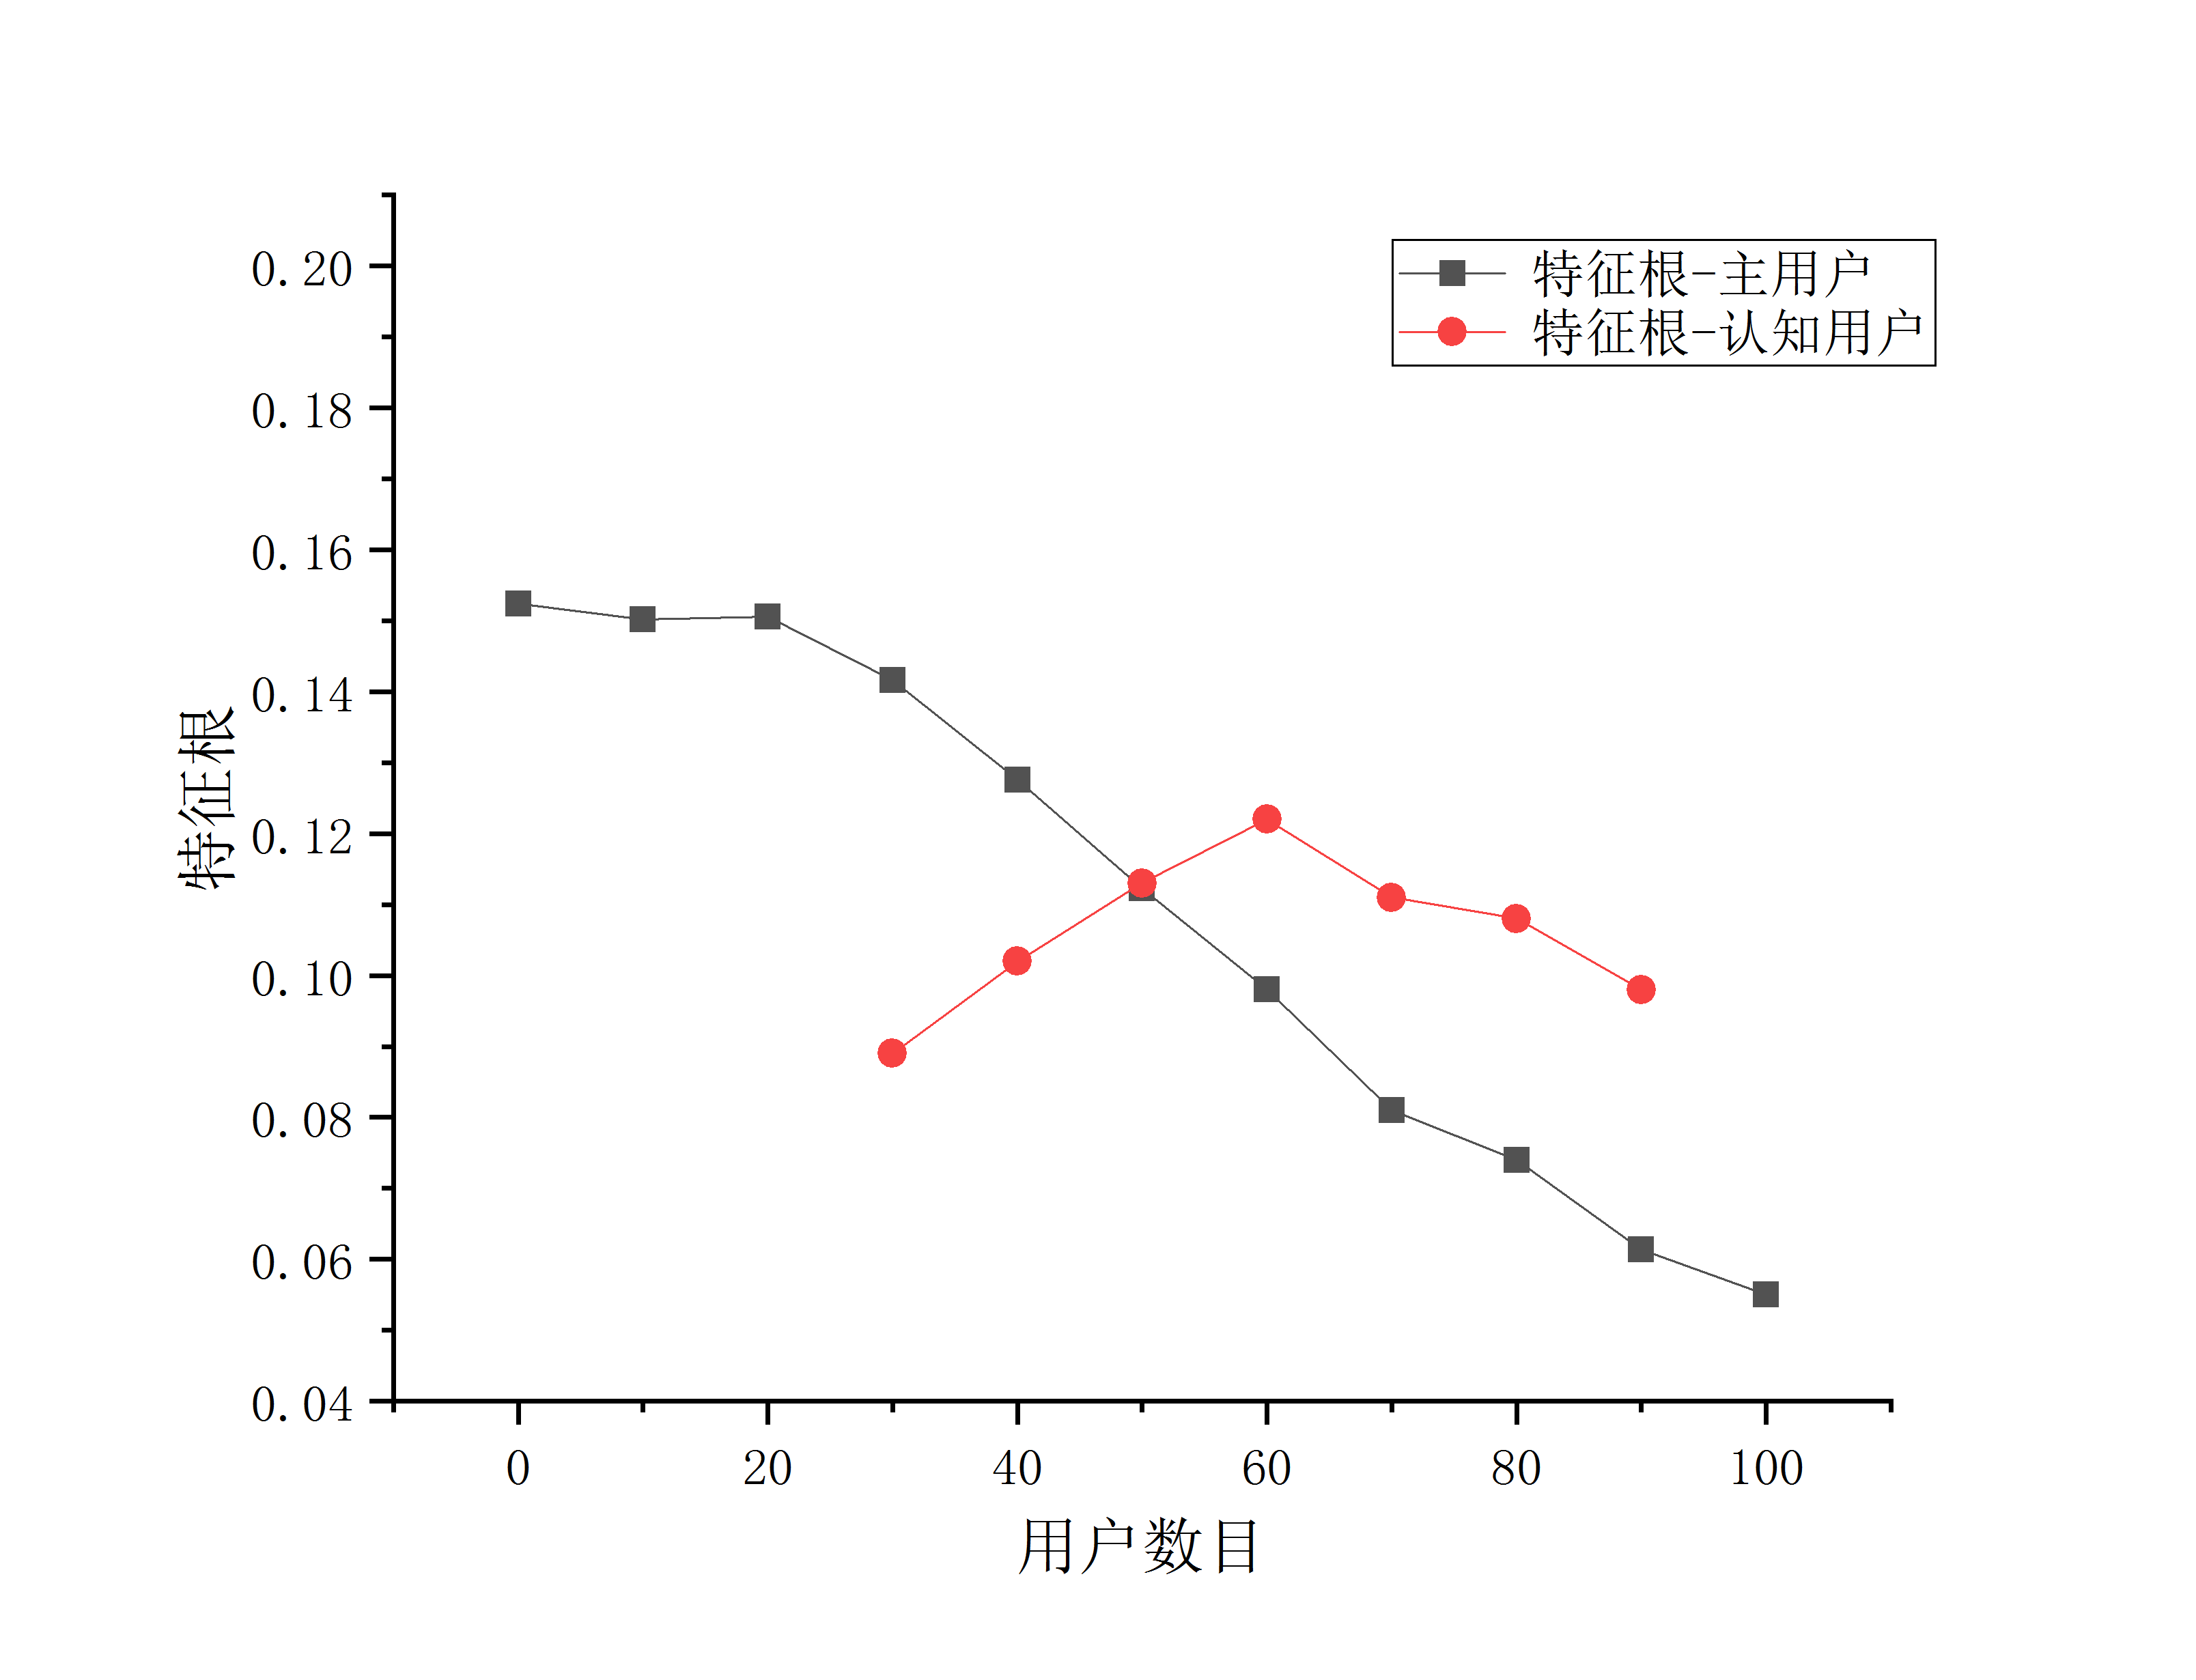
\includegraphics[scale=0.3]{pictures/pusu-strong.png} 
\caption{节点数目对网络健壮性的影响} %插入图片的标题,一般放在图片的下方,放在表格的上方
\label{pusu-strong}
\end{figure}

\begin{figure}[htbp]
\centering %使插入的图片居中显示
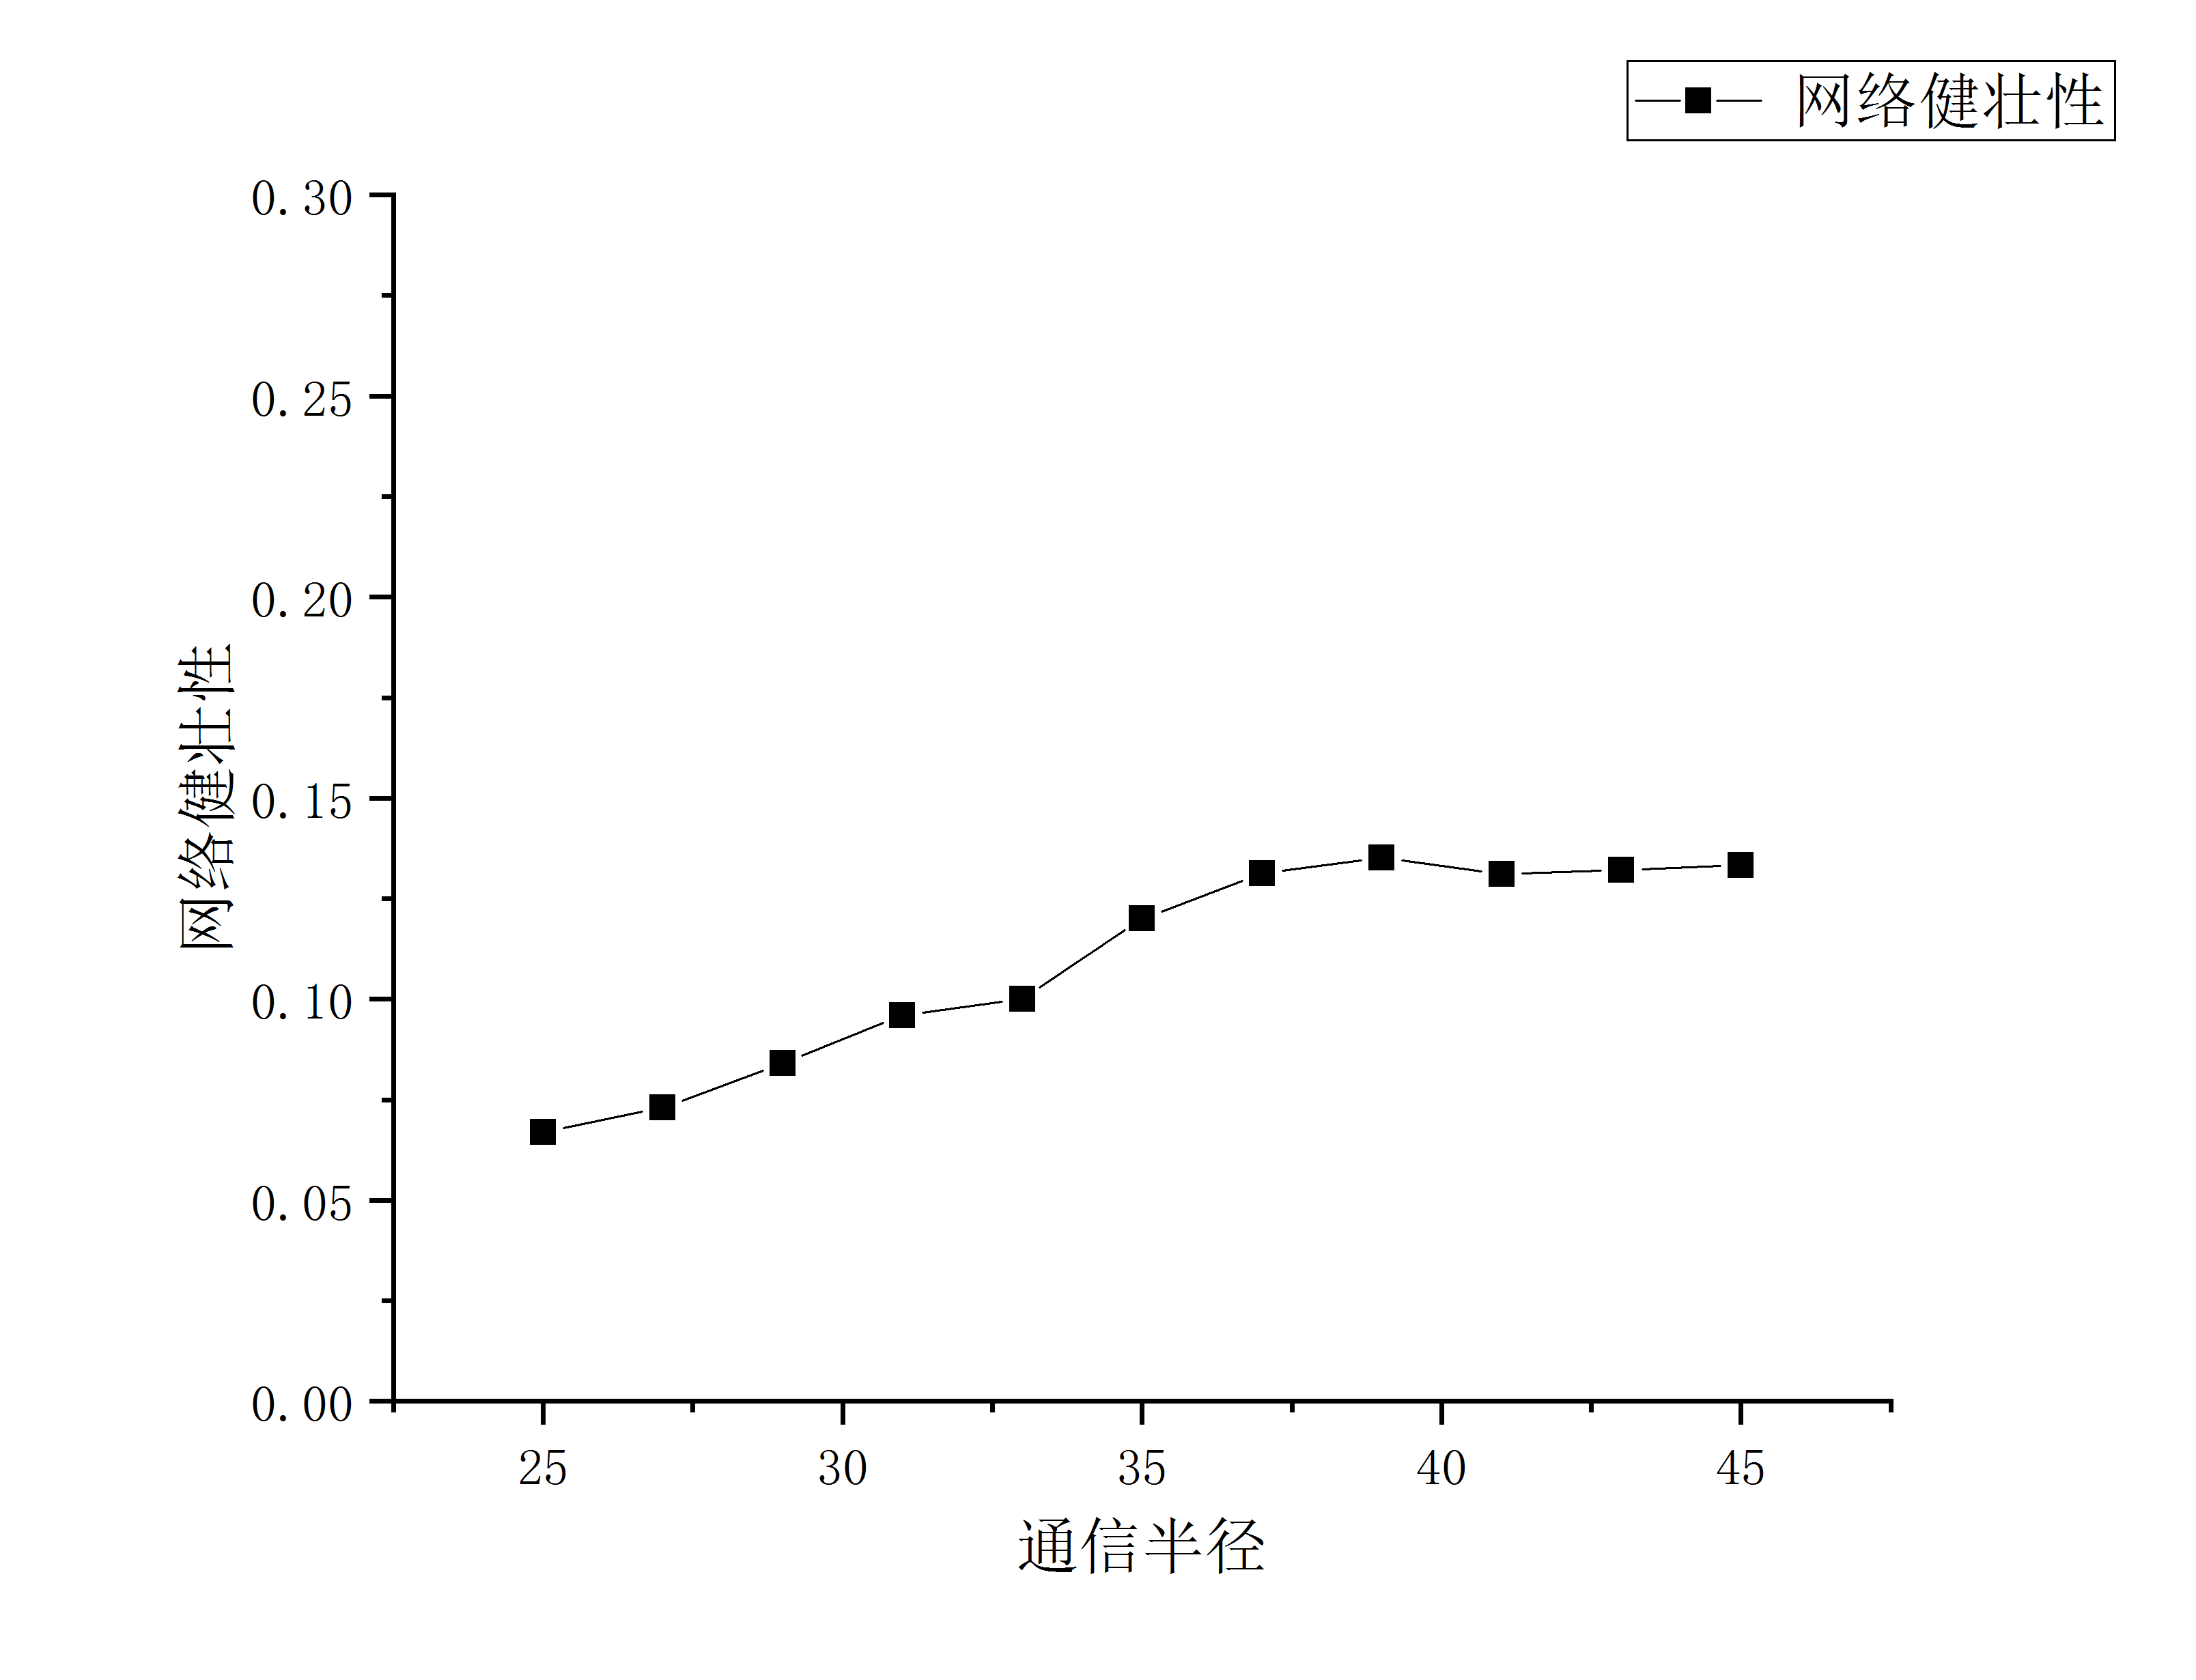
\includegraphics[scale=0.3]{pictures/R-STRONG.png} 
\caption{通信半径对网络健壮性的影响} %插入图片的标题,一般放在图片的下方,放在表格的上方
\label{R-STRONG}
\end{figure}
  图中可知,主用户作为干扰因素,其数量越多,组网后网络的健壮性越低,认知用户作为通信节点,初始阶段会因为节点数的增加使得整个网络的簇更容易相连,出现多个连通子图的情况减少,在认知节点不断增多后,网络健壮性又会下降,认知节点增多会使得子簇的深度加深,虽然也会增加网关节点的数目,但是深度影响增加还是使得网络的健壮性下降,不同节点之间点点连通的概率下降,而通信半径也会增加网络的健壮性, 减少子图出现概率,在增加到一定数值之后不再对健壮性产生过大影响,甚至使健壮性略微下降, 这种情况与信道减少以及深度增加相关。
 \section{路由与数据传送性能}
  \subsection{可用路由数目}
  可用路由条目的数目是保证数据能够成功发送的根本,在分簇网络中,节点间通信的最远方式为:簇内成员$\to$簇头$\to$网关节点$\to$ $\cdots$簇头$\to$簇内成员,由于分簇网络作为多跳网络,节点间的通信需要借助多个簇头与网关节点,而路由条目的数目保证了在某个簇头或者网关节点死亡的条件下依然可以选择其他通路进行通信。
  
  文中使用的路由寻找方法属于洪泛式路由,在路由寻找过程中一个比较严重的问题就是网络中将会出现过多的路由寻找数据包,这要求必须对每个路由寻找帧的寿命进行限制,以免在真实应用场景中造成网络拥塞,所以对于这个问题下面给出了路由寿命(路由寻找帧的跳数上限)与可用路由数目的关系,选择合适的网络路由寿命有利于整个网络的运行。
  路由寻找的过程,跳数越多,可以获得的路由将会越多,但是也会延长网络的整体路由发现时间,并且真实无线网络中多跳路由的生存类似于通信网课程中的生灭过程\cite{tongxinwang},其过程的状态转移图如图\ref{shengmie}所示
\begin{figure}[H]
 \centering 
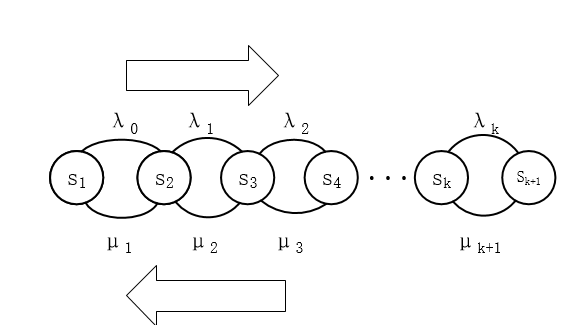
\includegraphics[scale=0.5]{pictures/shengmie.png} 
 \caption{路由状态转移表 
 }\label{shengmie}
\end{figure}


 
  令$\theta_0=1$,$\theta_k=\frac{\lambda_0\lambda_1\lambda_2\cdots\lambda_{k-1}}{\mu_1\mu_2\mu_3\cdots\mu_k}$ ,其中每个状态的$P_k=\theta_k P_0$  ,代表路由条目中簇头正常工作的数目。稳态分布下$P_0=\left(1+\displaystyle\sum_{i=1}^{\infty}\theta_k\right)^{-1}$,所以随着路由条目中经过的节点的数目增加将会同时增加路由条目失效的风险,因此在实际应用场景中对于跳数以及路由失效风险应该进行权衡的选择。
  
  仿真中给出了不同跳数下可以获得的路由条目数目以及程序运行的平均时间(c++中利用clock tick表示)的关系图\ref{luyoushumu},由于在T>6之后程序运行时间实在过长,所以随机选取了两个节点作为通信双方,并对他们的路由过程进行了平均计算,为了便于观察,对clock tick进行了取对数后缩倍处理,据此来观察路由协议的收敛时间,由于计算机模拟在超过8跳之后即使是两个节点采平均数的时间也是十分漫长,所以只观察8跳之前的路由状况。
  %\buptfigure{pictures/luyoushumu}{跳数与路由性能的关系}{luyoushumu}
   \begin{figure}[htbp]
\centering %使插入的图片居中显示
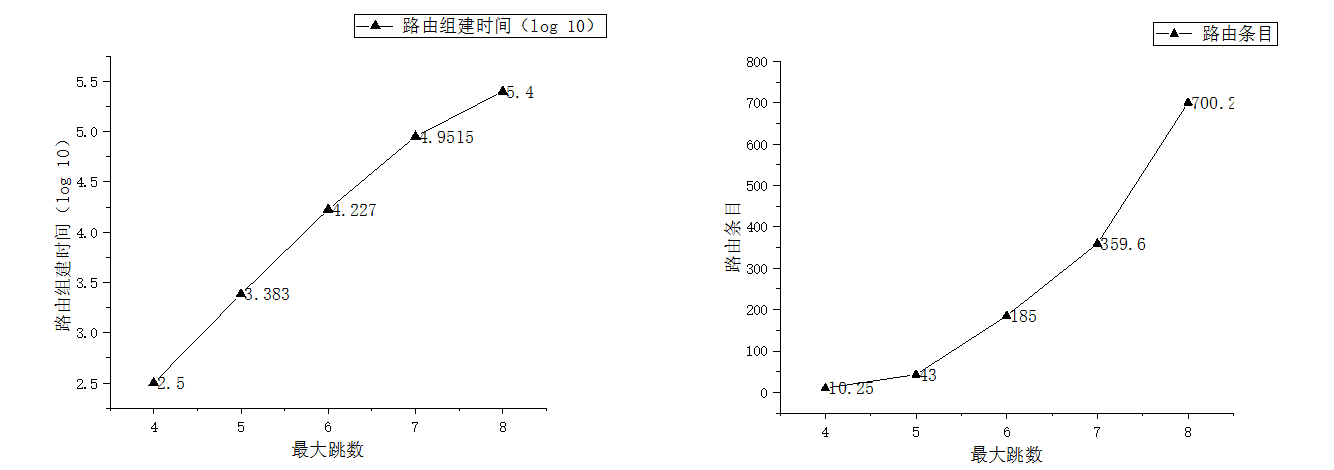
\includegraphics[scale=0.45]{pictures/luyoushumu.png} 
\caption{跳数与路由性能的关系} %插入图片的标题,一般放在图片的下方,放在表格的上方
\label{luyoushumu}
\end{figure}
  根据仿真结果中可知,整体网络的路由过程运行时间与最大跳数成正比关系,且随着跳数增长,消耗的时间也会呈现指数型增长趋势,而路由条目同样也与最大跳数的幂函数成正比,这是因为跳数的增加意味着可以经过的簇头数目与网关节点数目增加,而并非简单地加法,是与簇头及网关节点的次幂函数相关。图中我们也可发现,这两者的优势不能同时具备,要向获得更多的路由条目意味需要消耗更多的组网时间。
  
  分簇网络中的路由与分簇数目有着密切的关系,由于节点通信过程中会使用簇头和网关节点作为中间跳点,所以成簇的个数一定程度上影响了路由的跳数以及路由的可靠性,在文中成簇的个数主要受通信范围以及认知设备的密度(数目)的影响,下图\ref{fig:1}以及图\ref{fig:2}中给出了路由条目的数目与通信半径和认知节点数目的关系以及两者与成簇数目的关系,考虑到通信半径过大时组网成功率将会到达最大概率后降低,所以只考虑单调增区段的通信半径与路由数目的关系。
 \begin{figure}[htbp]
\centering  
 \subfigure[认知节点与成簇数目关系]
 {                   
\begin{minipage}{7cm}
\centering
  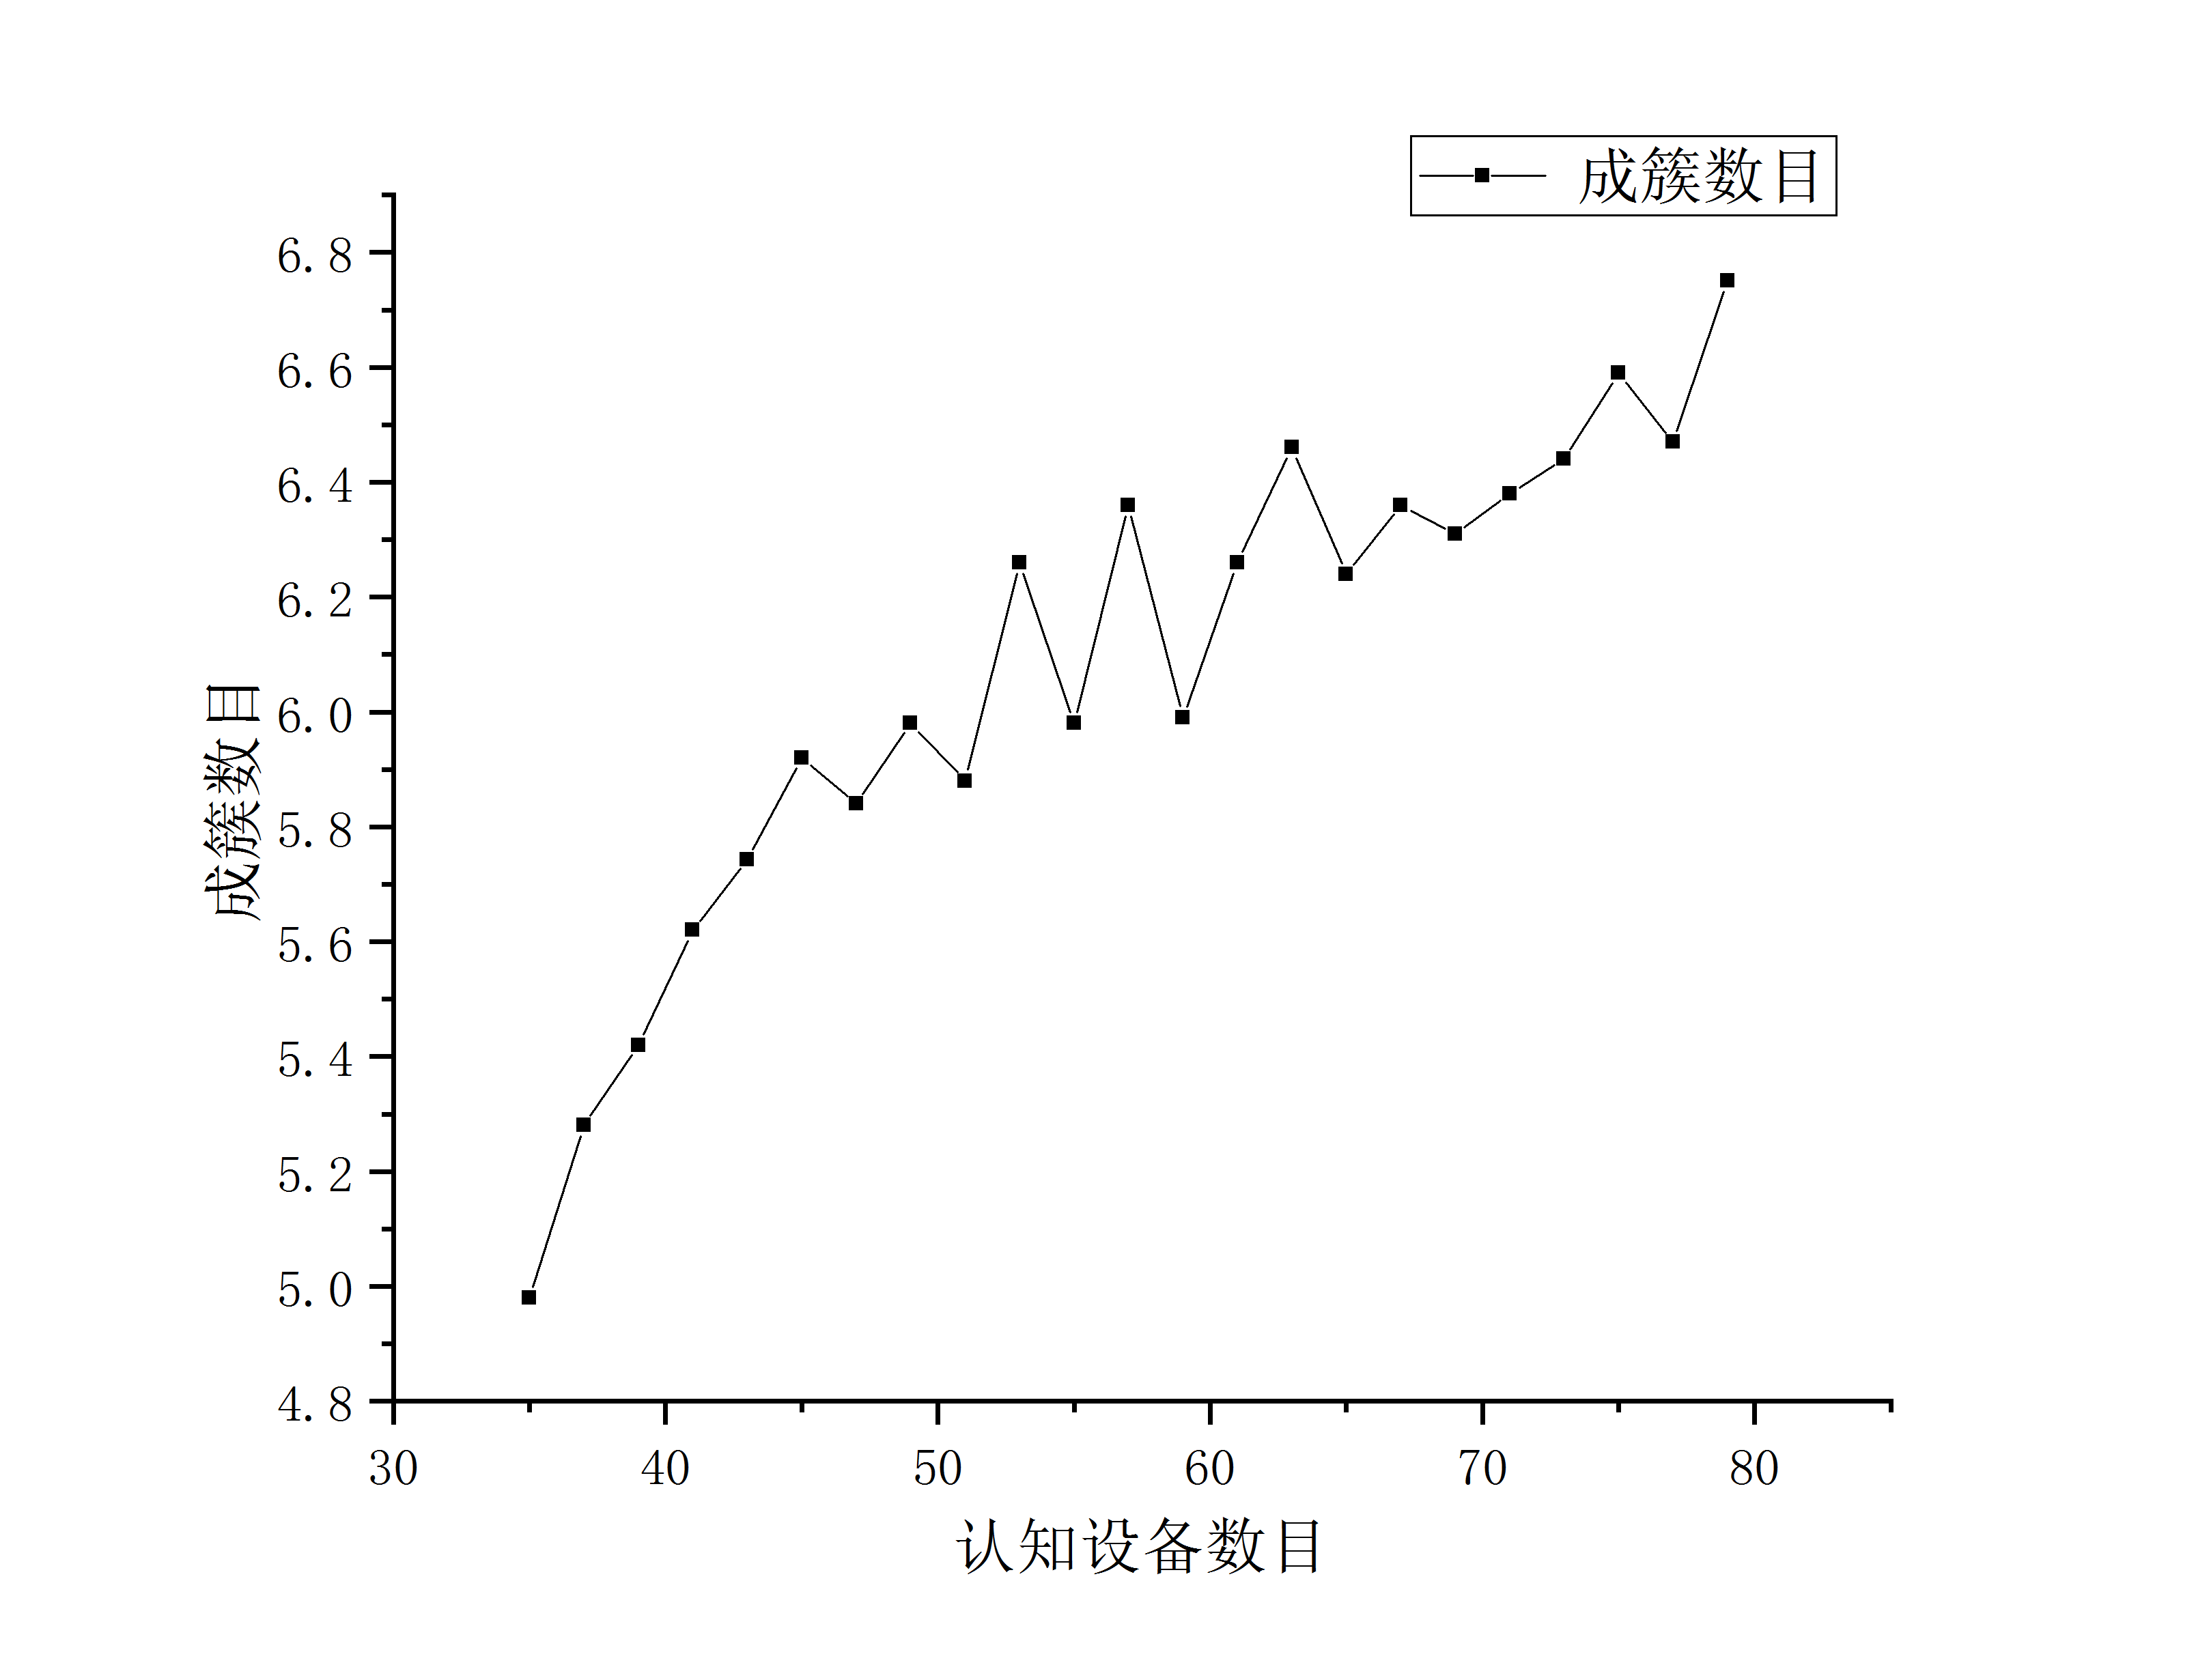
\includegraphics[scale=0.3]{pictures/CR-CL.png}   
  \end{minipage}}   
  \subfigure[认知节点与路由数目关系]{              
  \begin{minipage}{7cm}
  \centering                                                         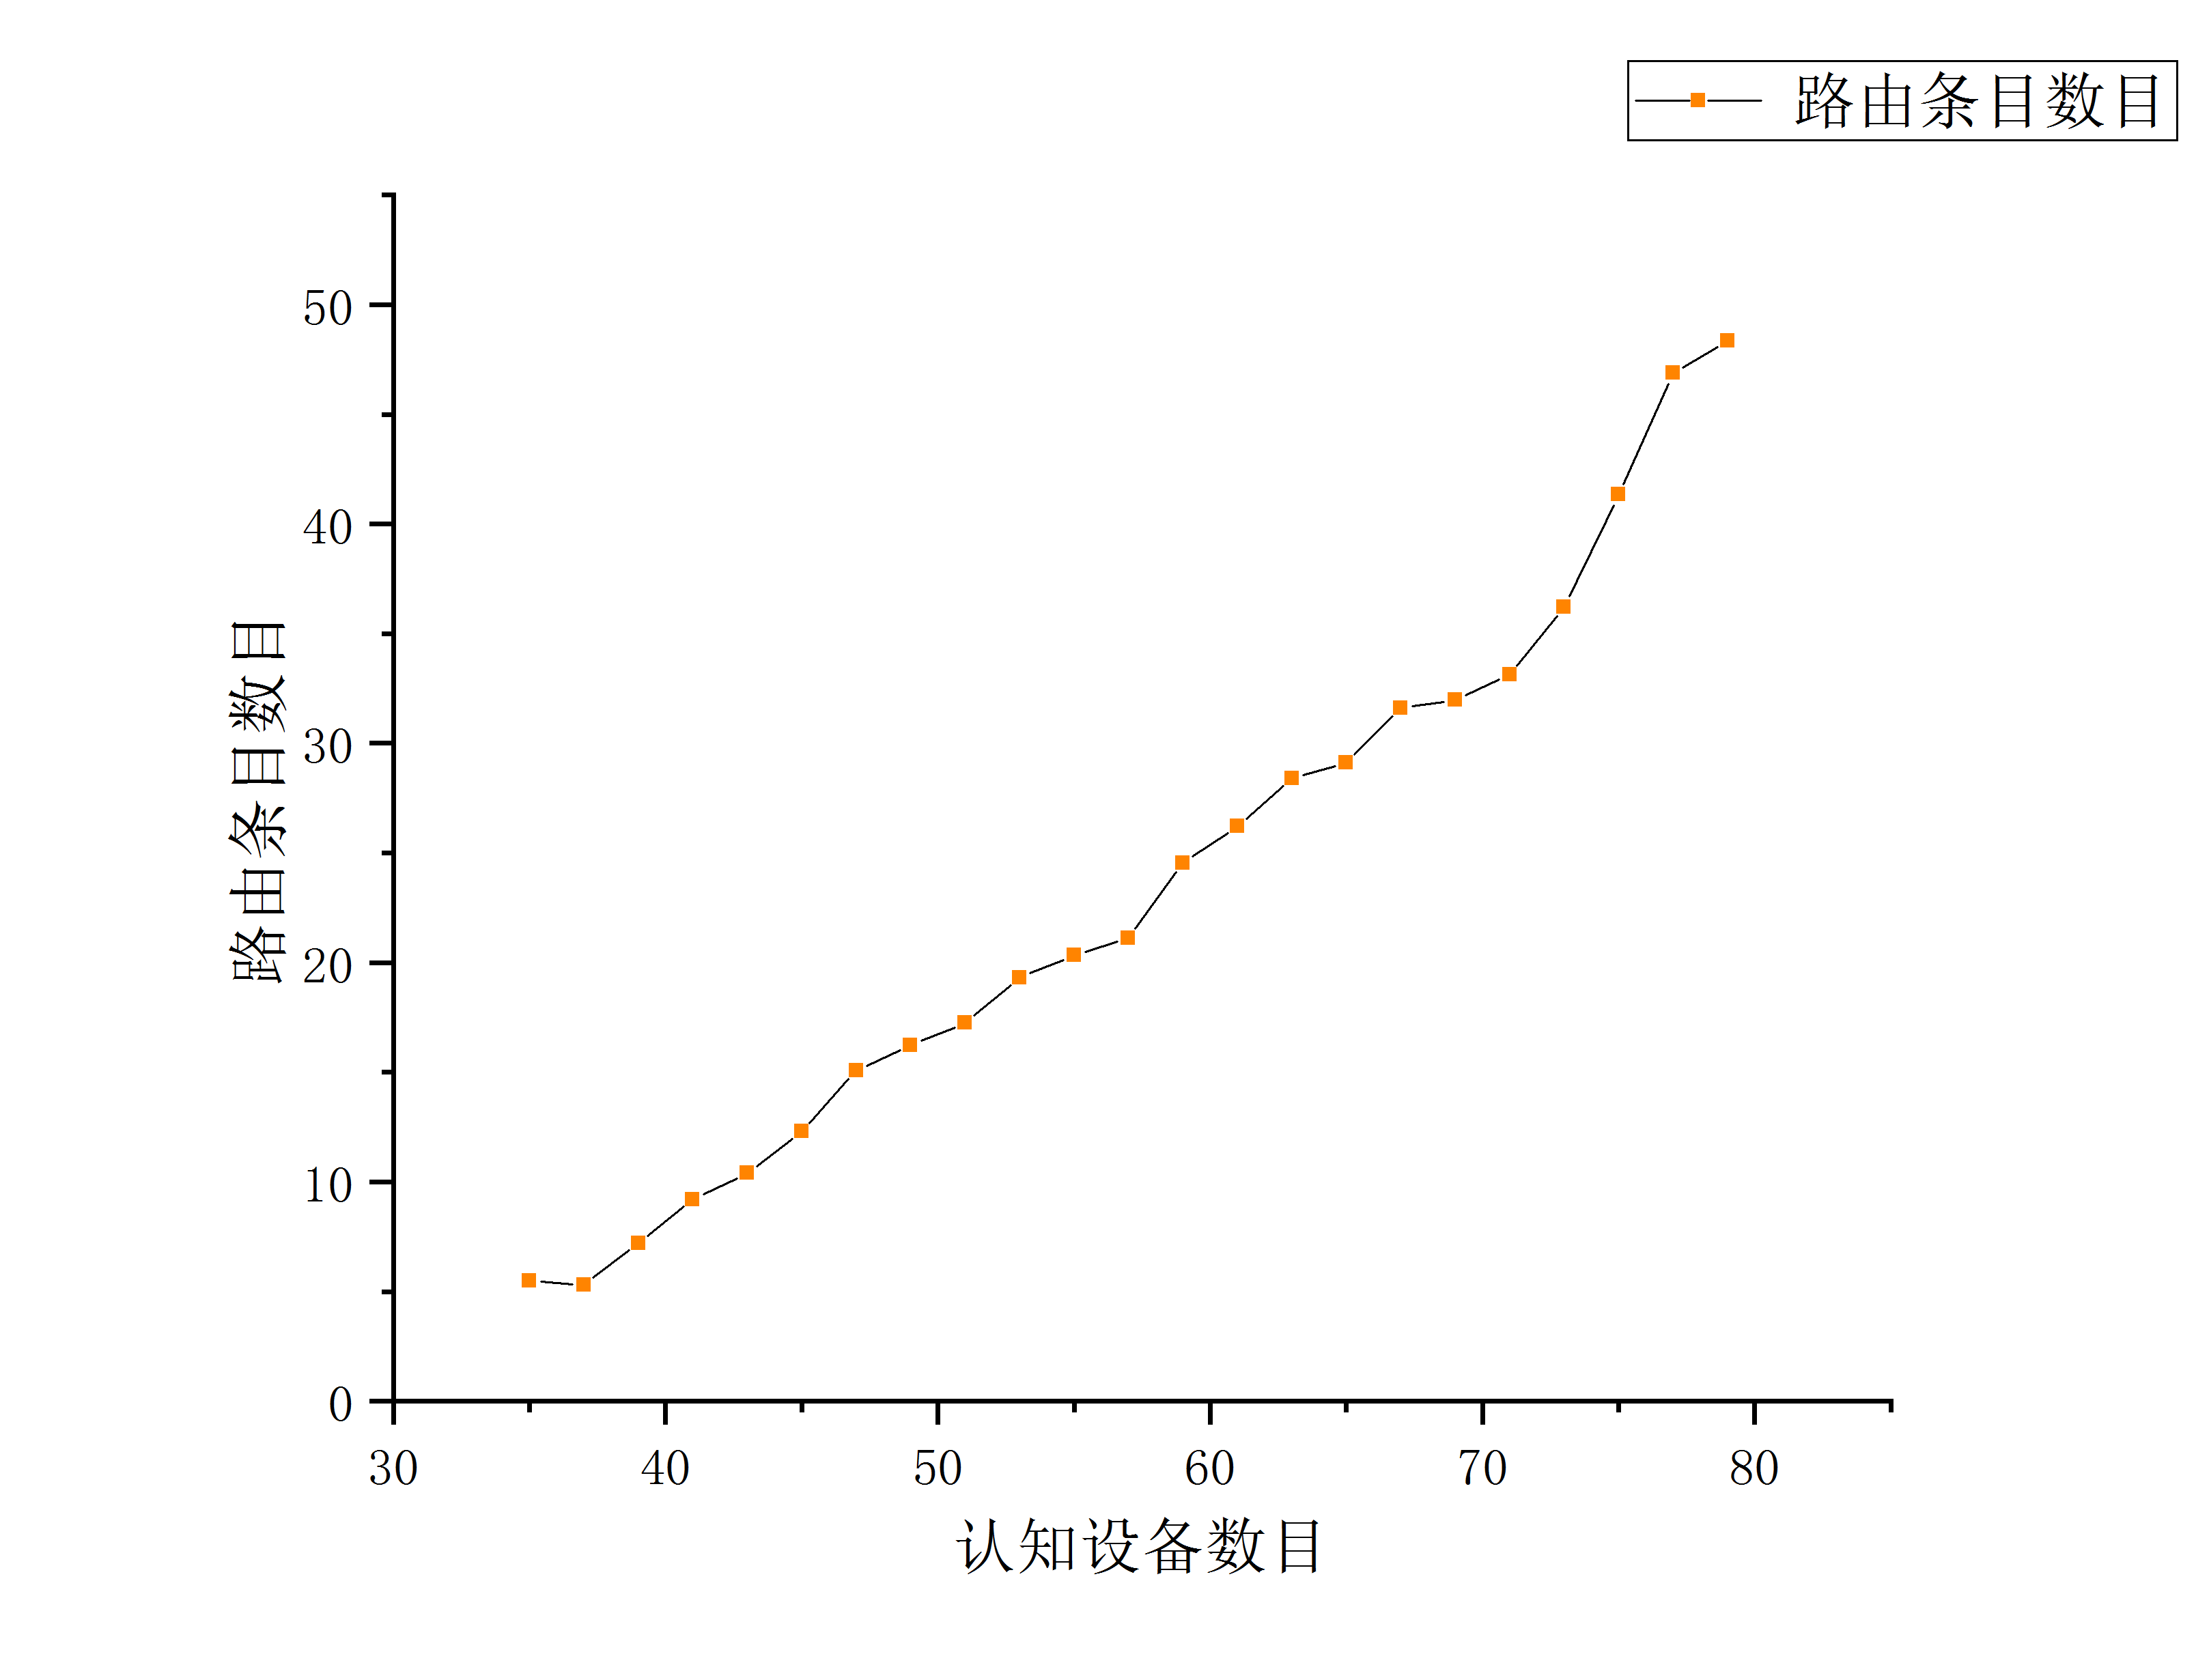
\includegraphics[scale=0.3]{pictures/CR-ROUTING.png}          
  \end{minipage}}
  \caption{认知节点数目对路由的影响}  
  \label{fig:1}                                                        \end{figure}
  图中可知,随着认知节点的增加,整个成簇的数量减少,意味着成簇深度的增加,而路由条目数目也随着认知节点数目增加而增加,证明网关节点的增多,产生了更多的路由条目,而通信半径的增加也同样增加了网关节点的数目,虽然网络健壮性下降但是路由数目却不断增加。
\begin{figure}[htbp]
\centering  
 \subfigure[通信半径与成簇数目关系]
 {                   
\begin{minipage}{7cm}
\centering
  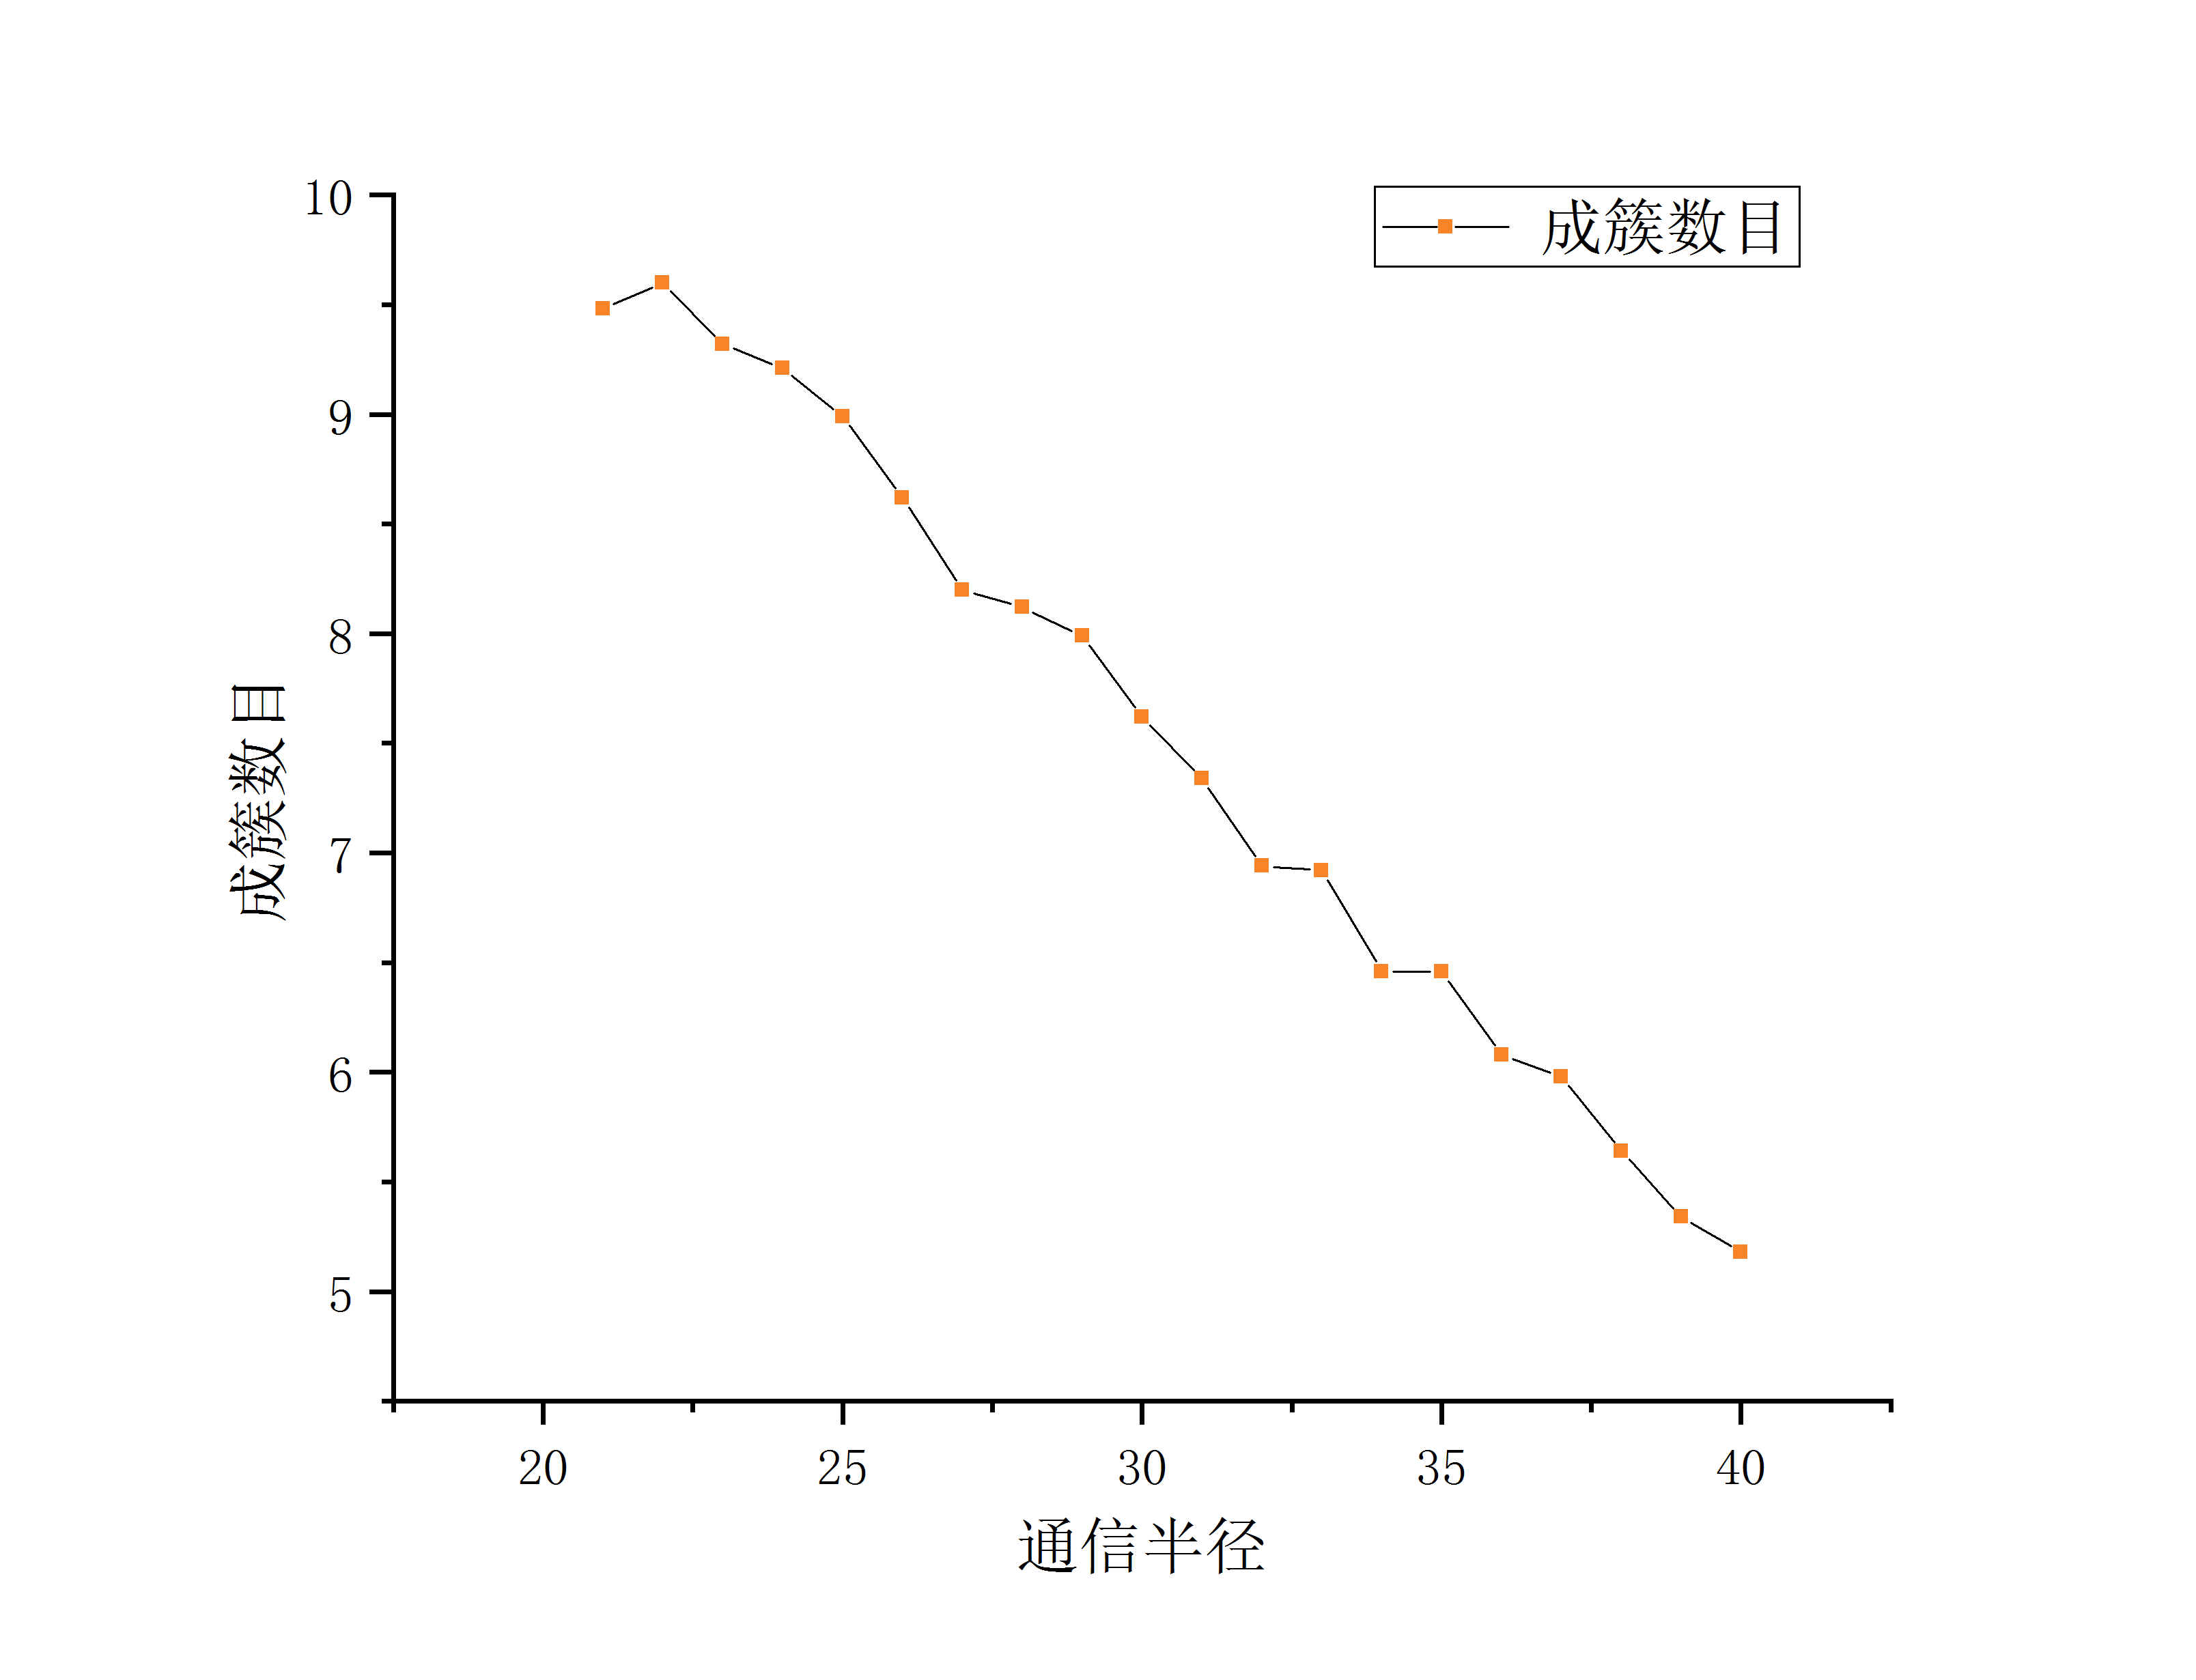
\includegraphics[scale=0.3]{pictures/R-CLUSTER.png}   
  \end{minipage}}   
  \subfigure[通信半径与路由条目关系]{              
  \begin{minipage}{7cm}
  \centering                                                         
  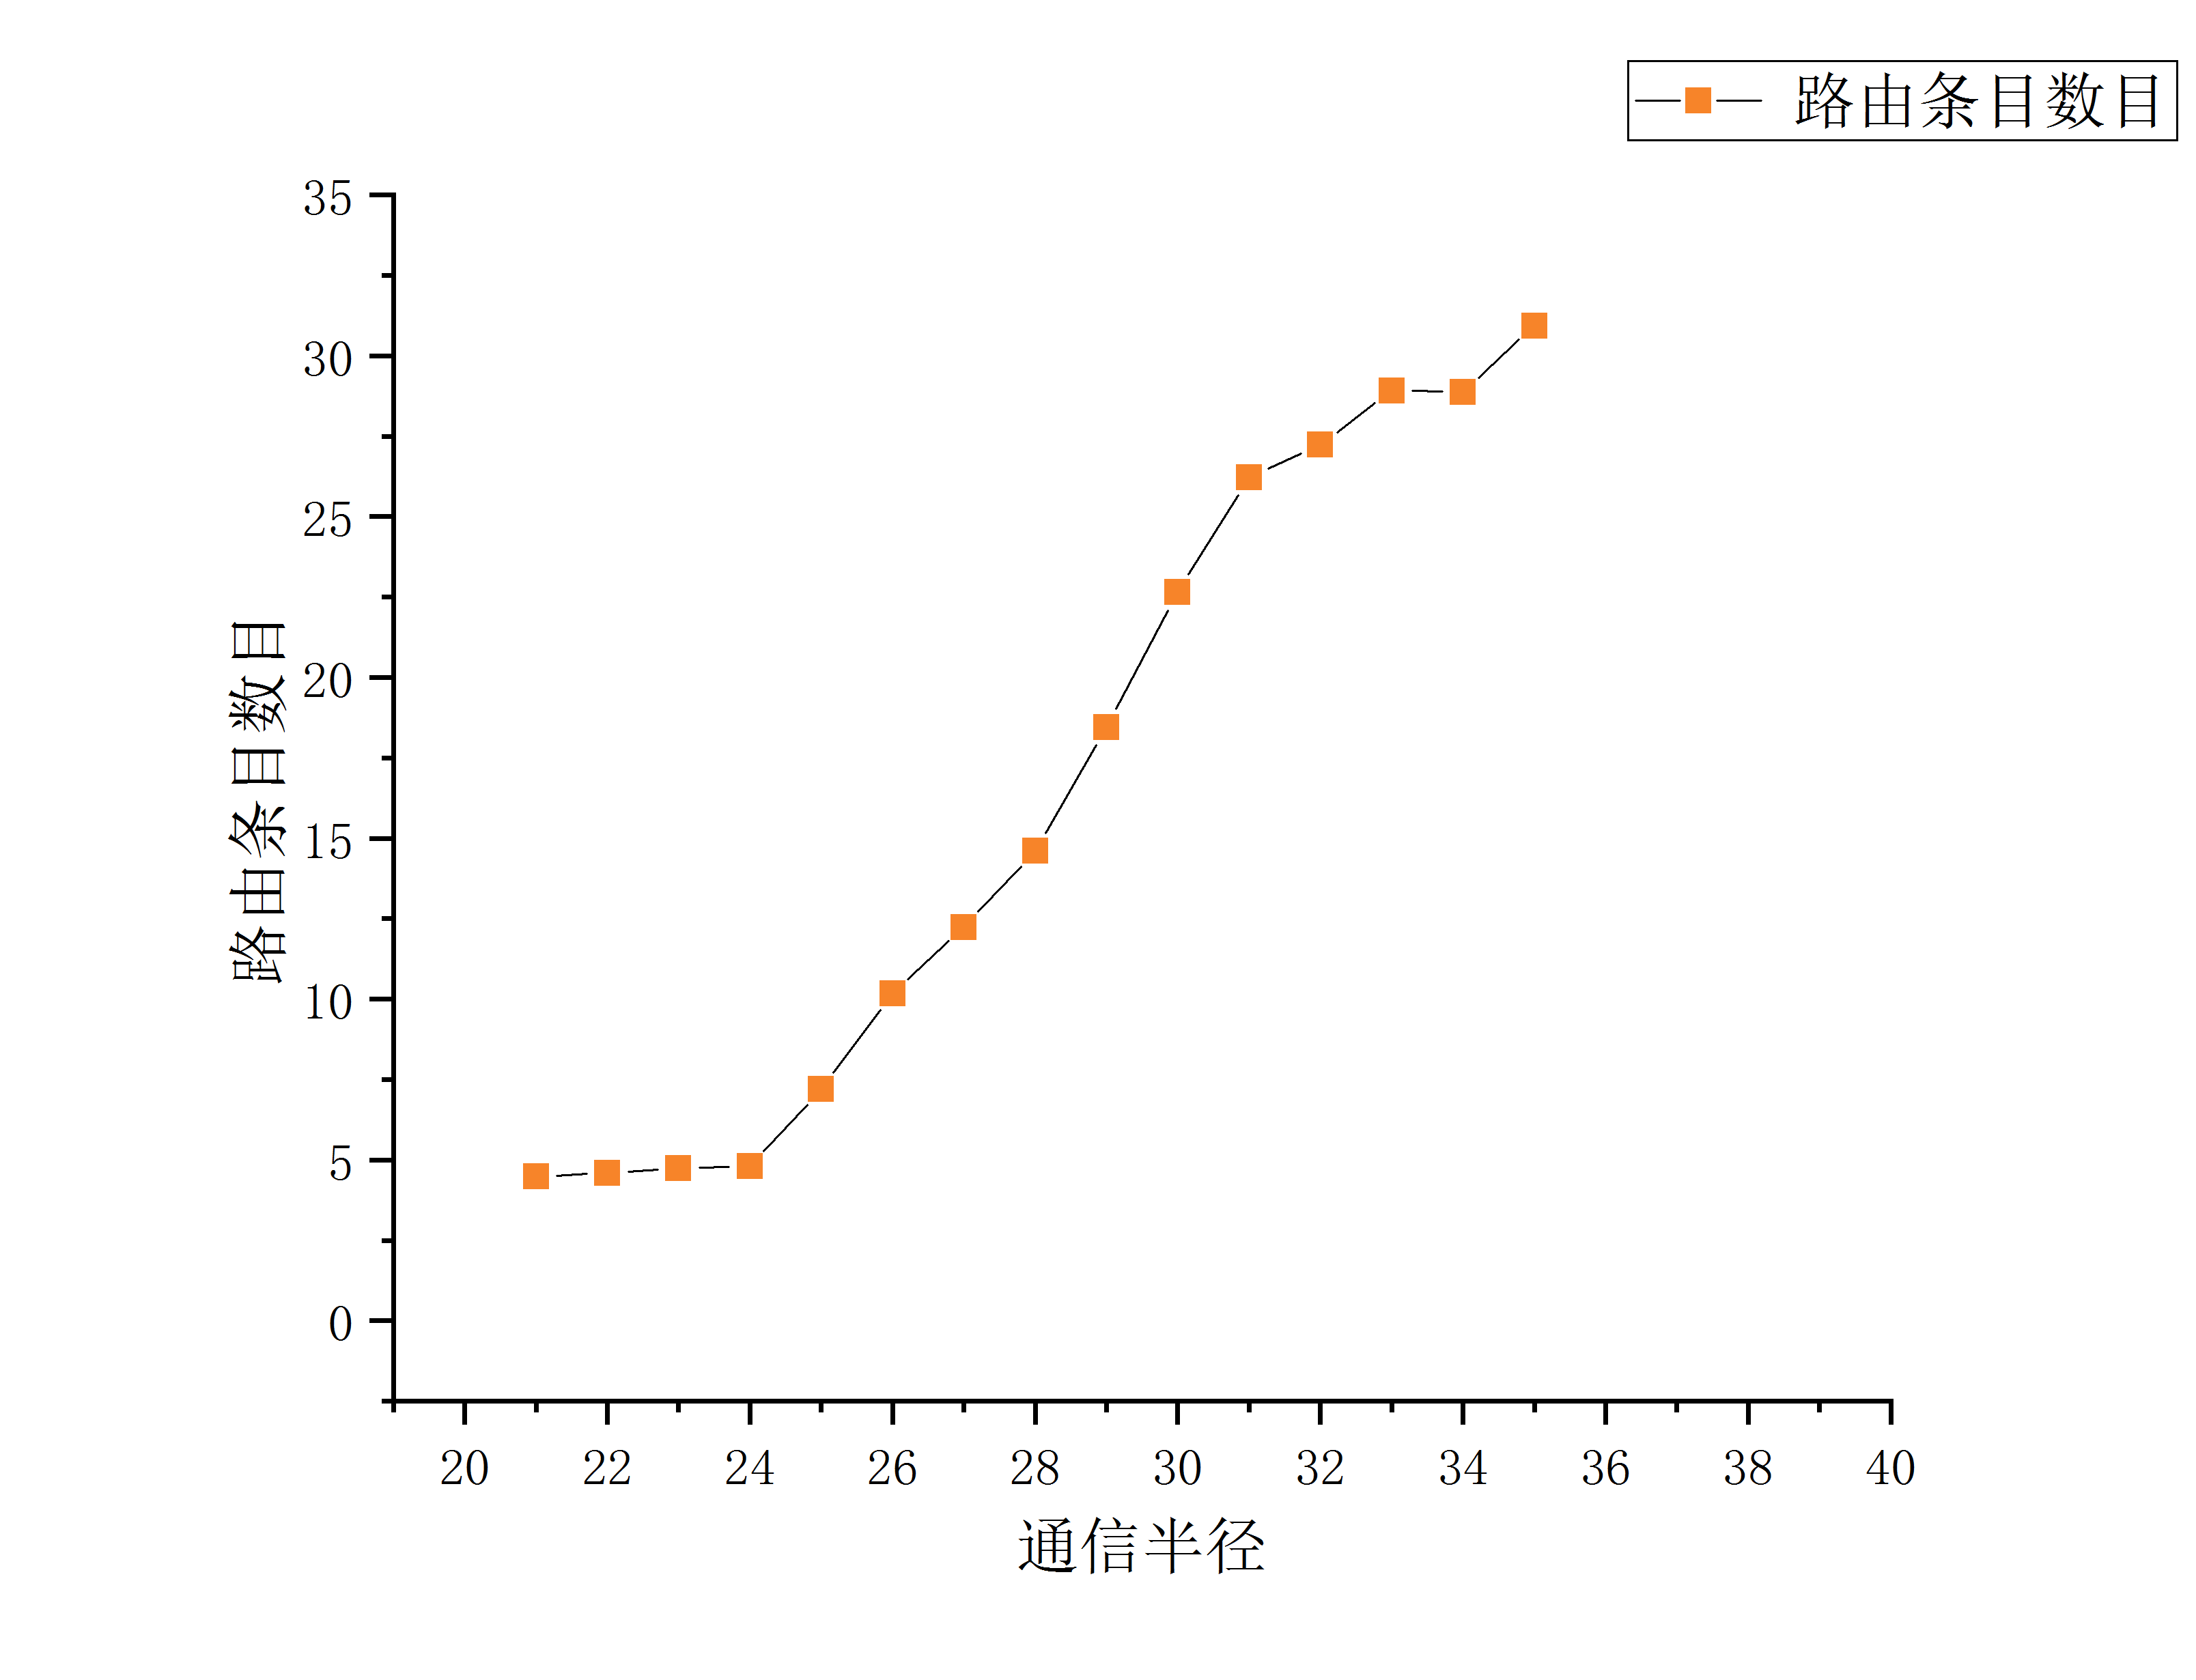
\includegraphics[scale=0.3]{pictures/R-routing.png}          
  \end{minipage}}
  \caption{通信半径对路由的影响}  
  \label{fig:2}               
   \end{figure}
   
  \subsection{网络平均寿命}
  文中给出了两种路由策略,一种先验式路由协议,一种按需路由协议,这两种路由策略的应用场景有所区别,在数据传送活动较少的区域,按需路由协议理因为其实时性的特点,应当有着更加优秀的能耗,在数据传送活动较多的区域,先验式路由协议可以节省大量路由数据包,从而获得更佳的能耗比。图\ref{energyextra}中给出了不同数据活动比(活动时间占总系统运行时间的比例)下的两种路由模式的能耗比例
   \begin{figure}[htbp]
\centering %使插入的图片居中显示
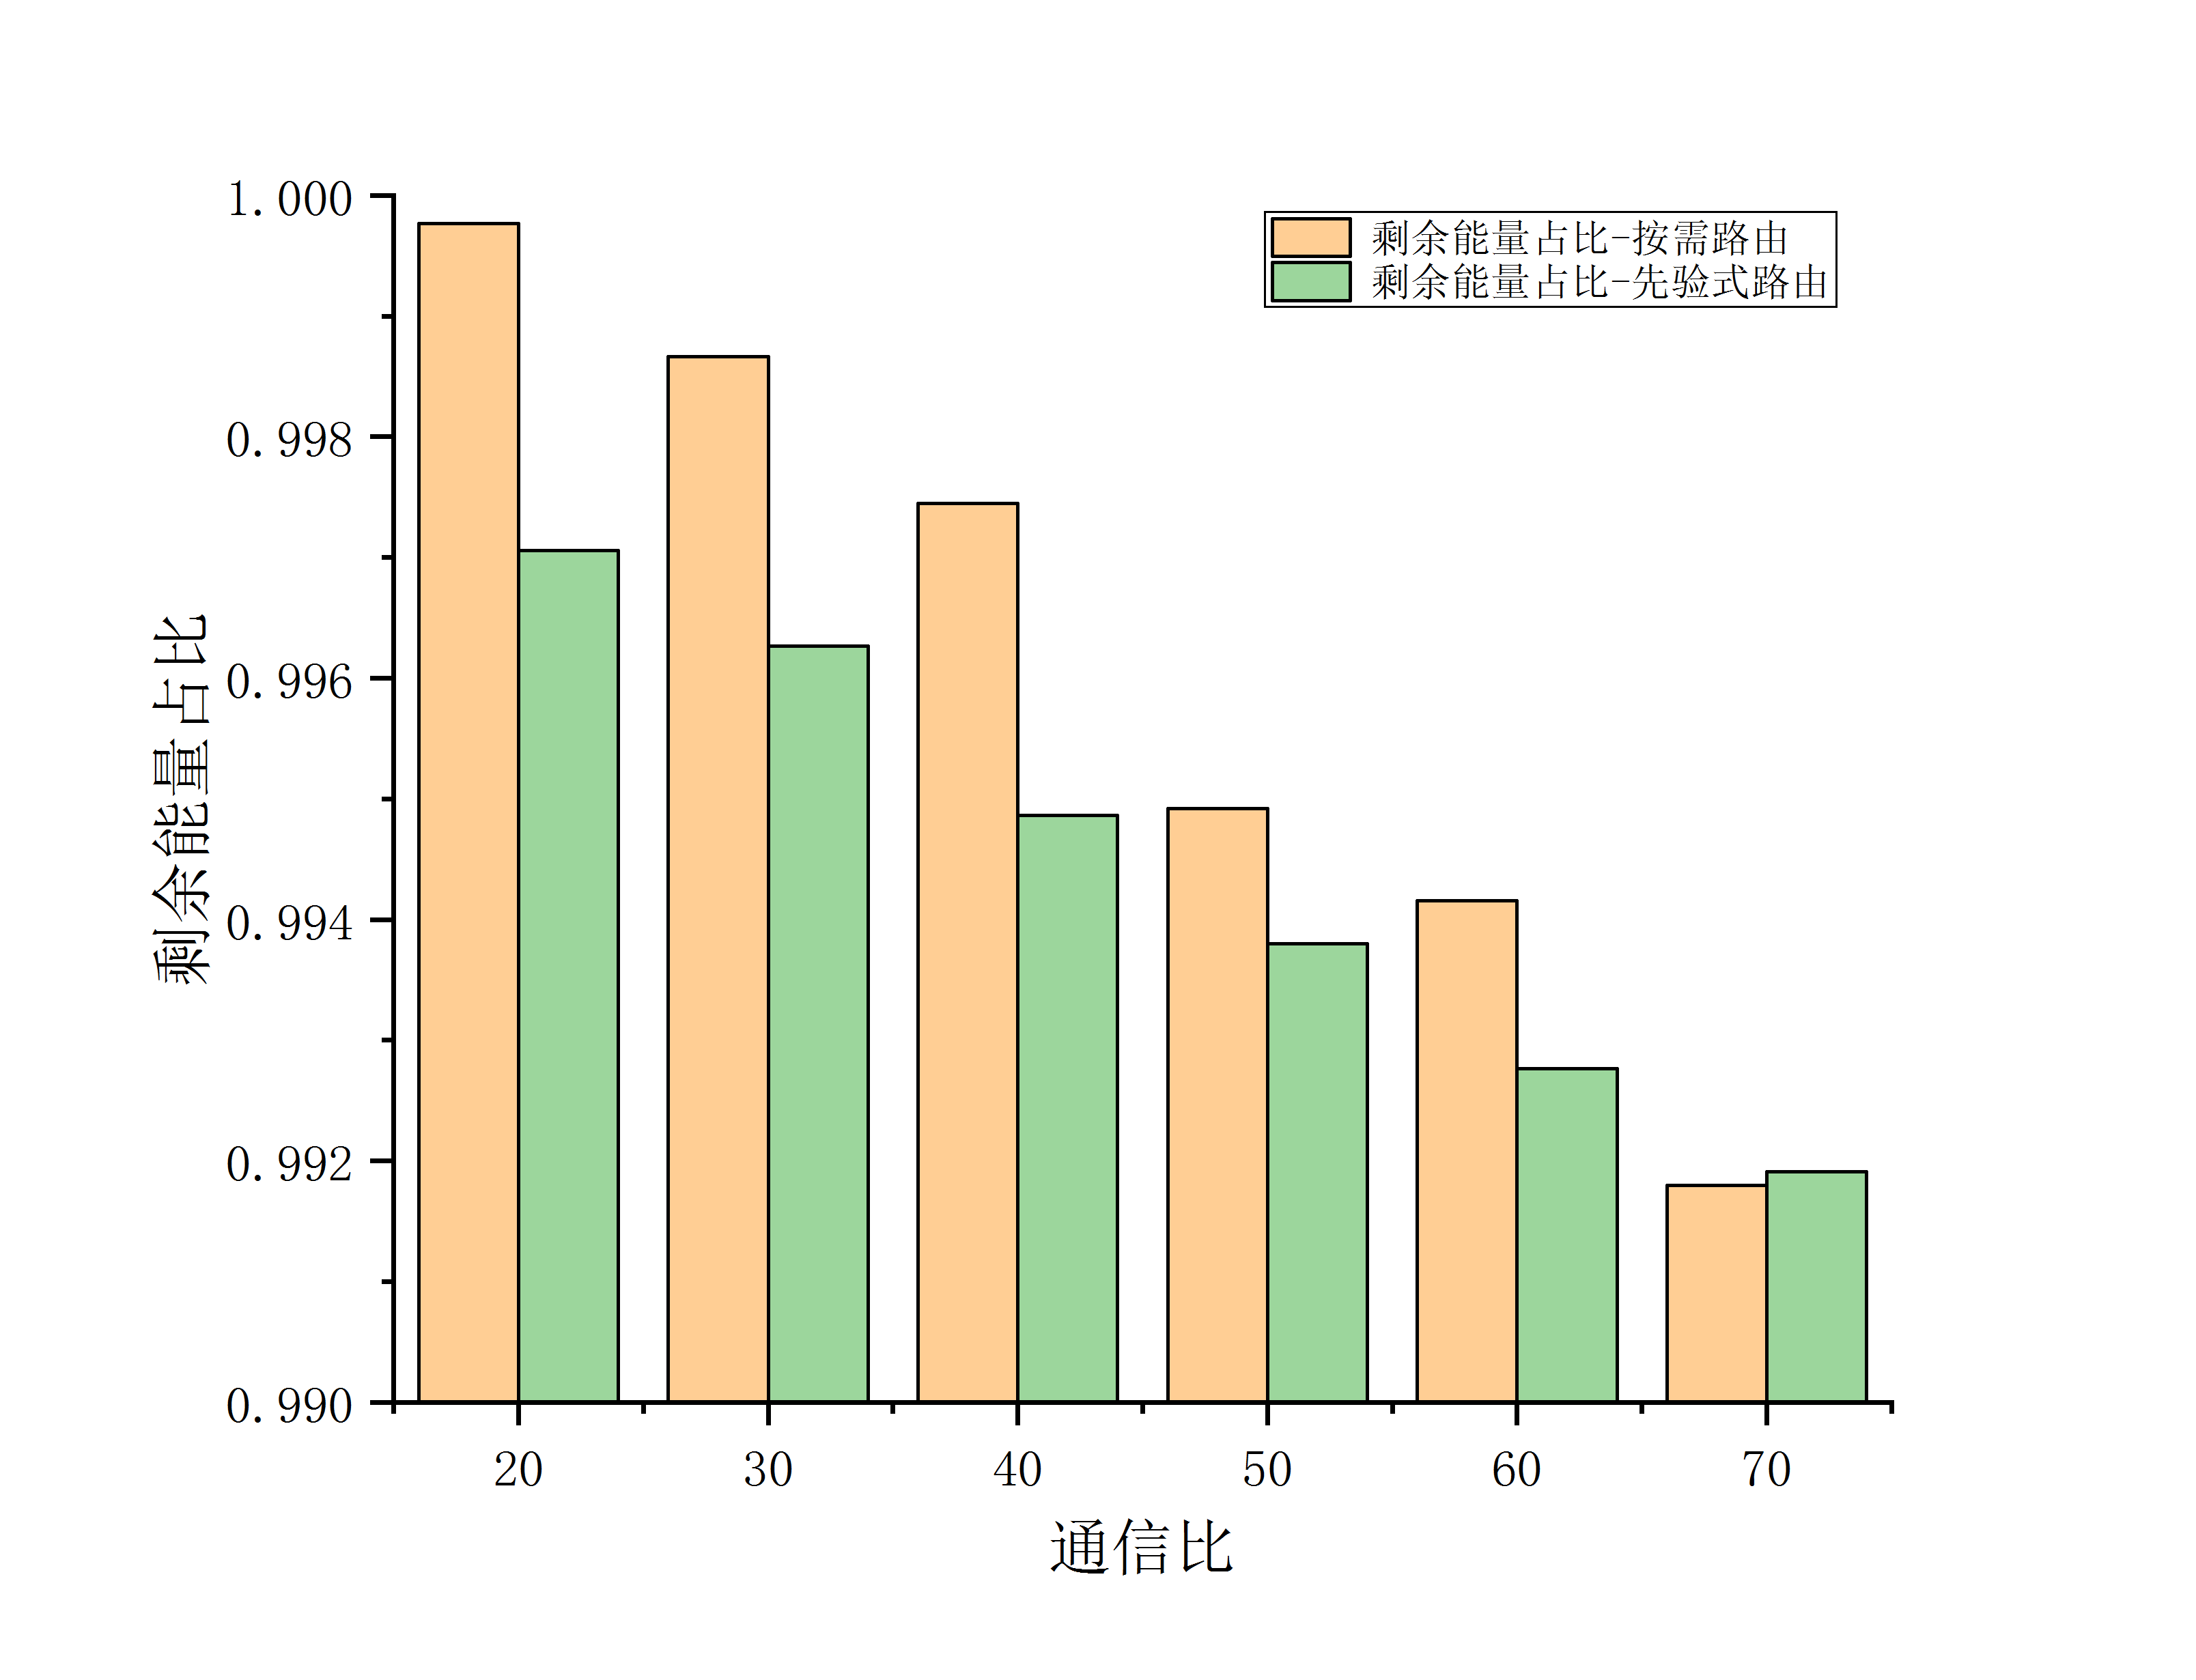
\includegraphics[scale=0.3]{pictures/energyextra.png} 
\caption{路由类型与剩余能量比例 } %插入图片的标题,一般放在图片的下方,放在表格的上方
\label{energyextra}
\end{figure}
  由图可知,按需路由协议在进行少量通信的时候可以节省更多能量,大于70的活动时间比时能耗将会高于先验路由协议,所以在数据活动剧烈的区域应当优先使用先验式路由协议,相反则优先使用按需路由协议。
  \subsection{传送数据类型}
  对于网络中不同的数据类型要求,适当的路由选择方式可以有效延长整个网络的节点运行时间。所以给出了两种数据包类型,一种低时延数据包和一种最长网络寿命数据包。低时延数据包由于会长时间使用最短时延线路,将会先出现死亡节点,通过观察第一个死亡节点的出现时间,可以估计整个网络的寿命,所以代码实现中,会对所有节点初始能量设置为随机数。图\ref{datatype-die}中给出了首次出现节点死亡的时间对比。
 
  \begin{figure}[htbp]
\centering %使插入的图片居中显示
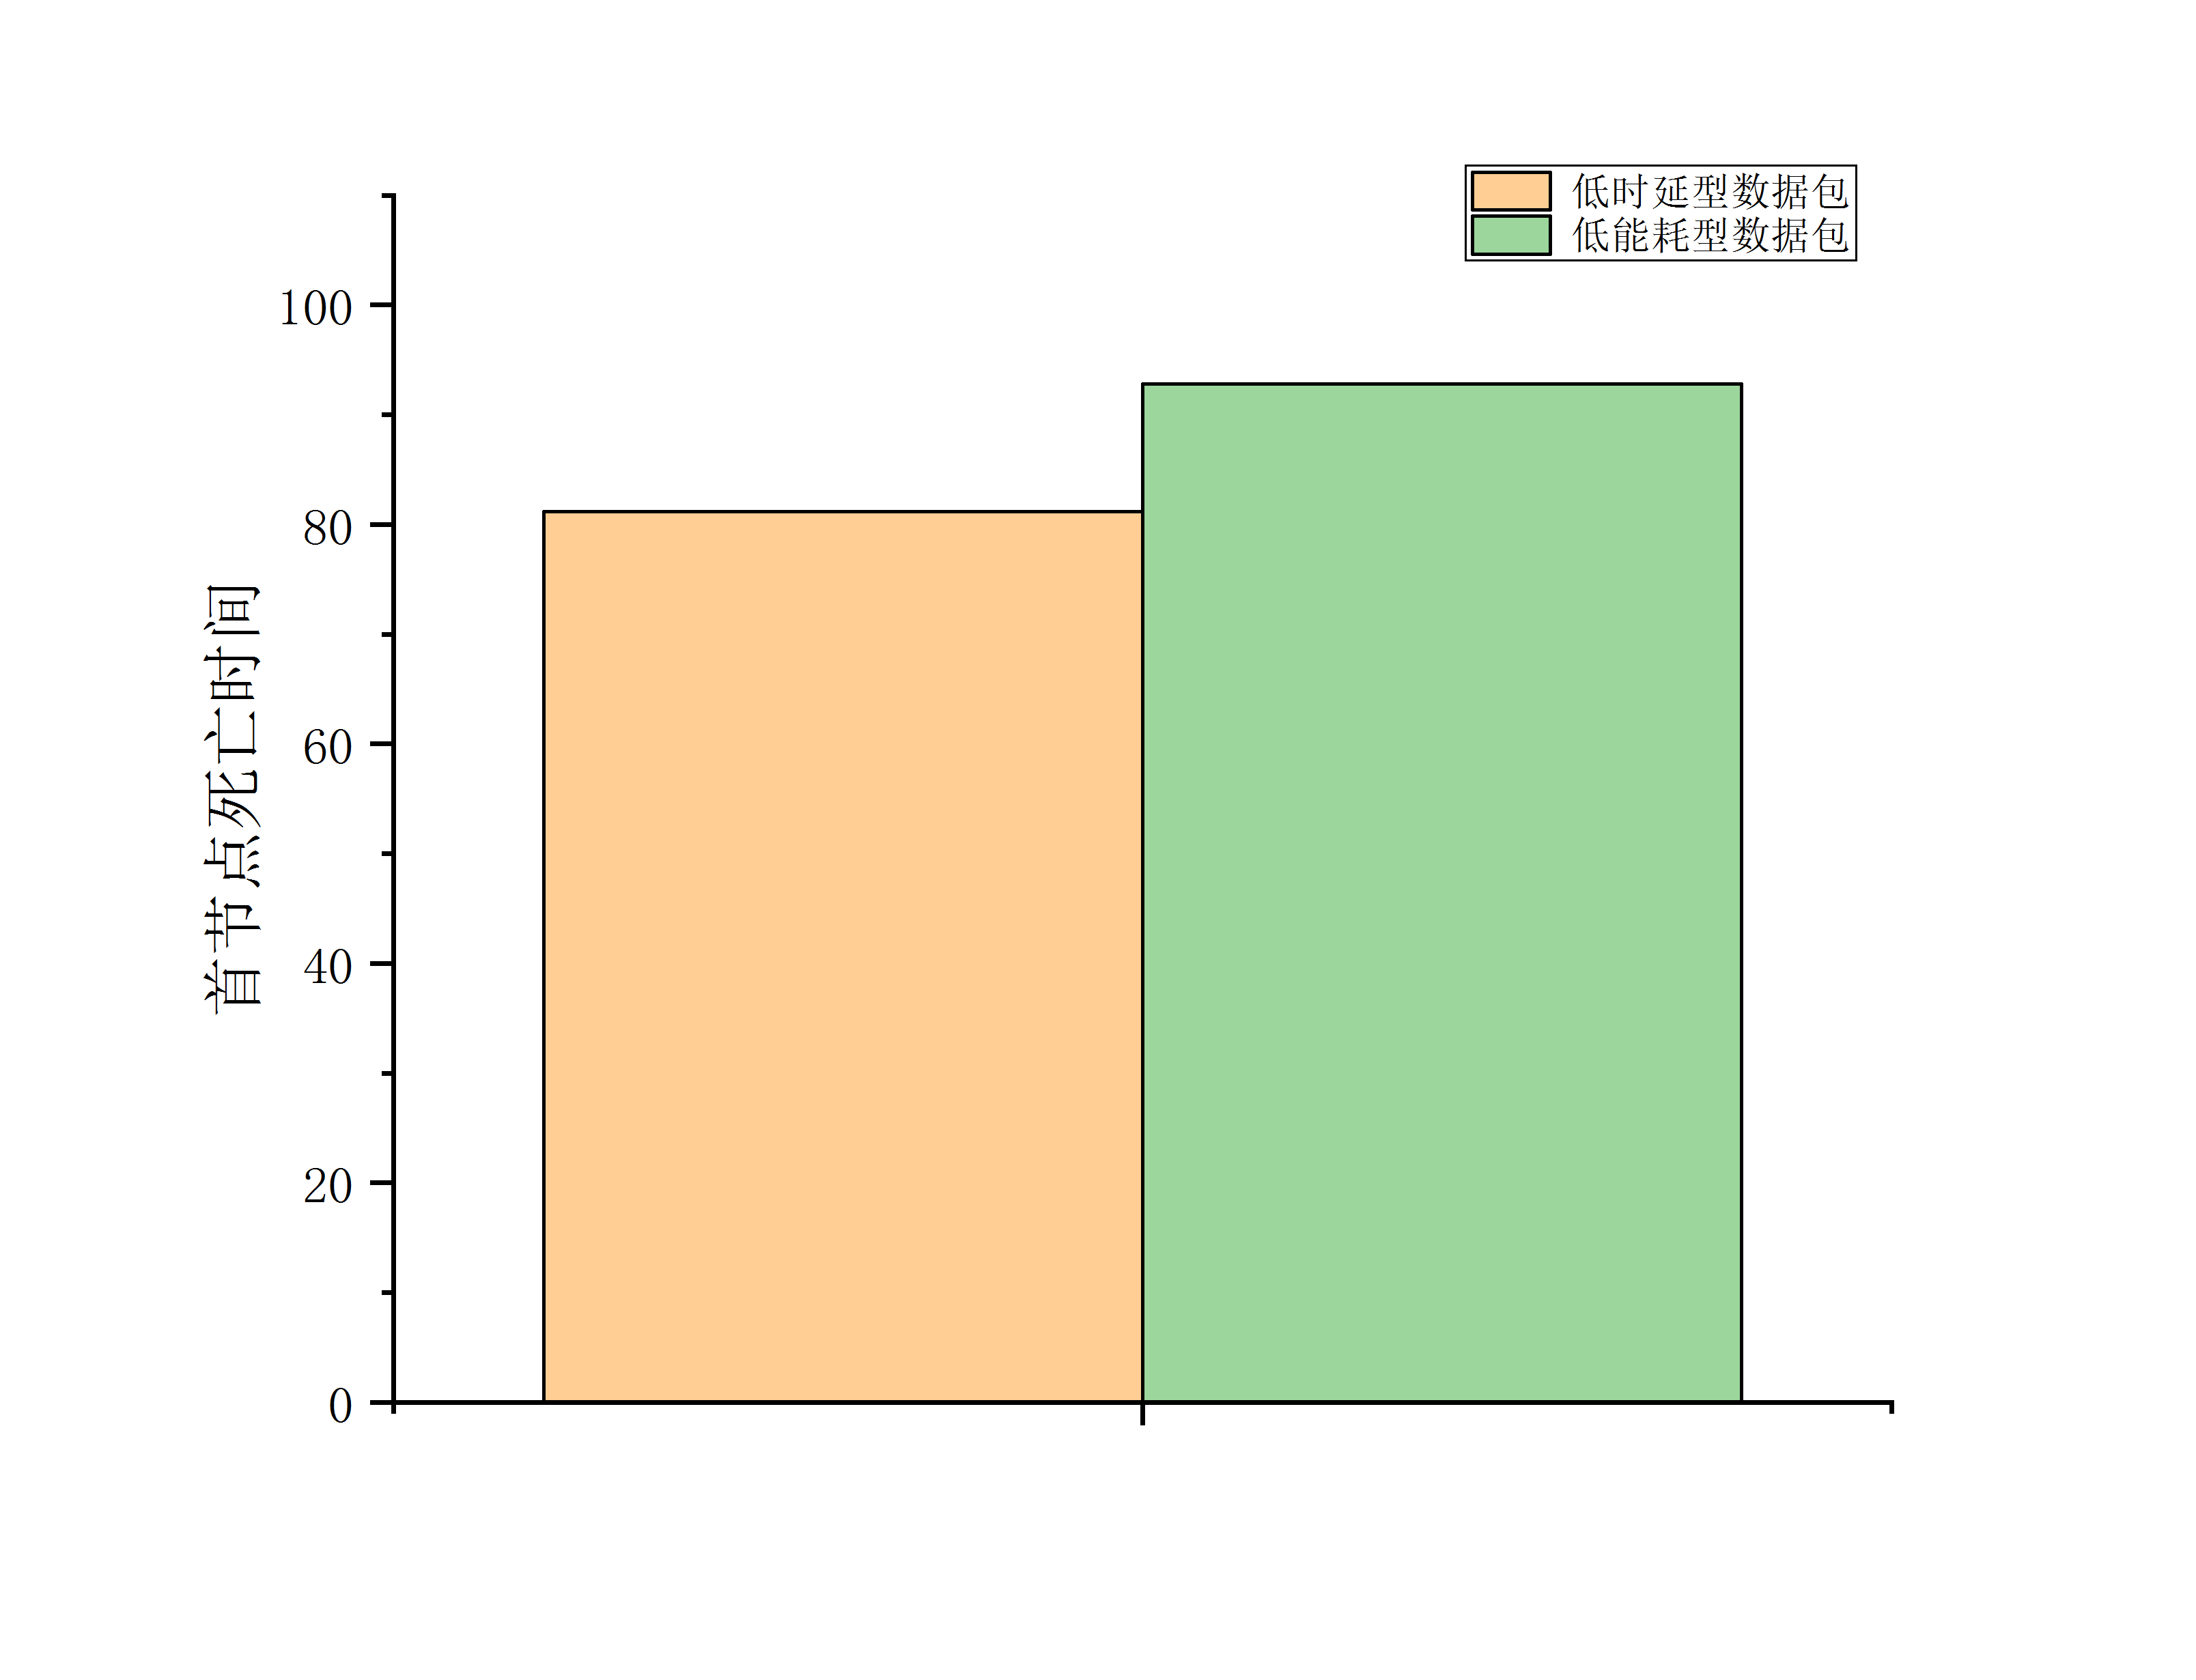
\includegraphics[scale=0.3]{pictures/datatype-die.png} 
\caption{数据包类型与首节点死亡时间对比 } %插入图片的标题,一般放在图片的下方,放在表格的上方
\label{datatype-die}
\end{figure}
  图中可以看出,使用第二种路由方案可以有效延长首个节点死亡时间,同理可以增加整个网络的平均寿命,但是这是以不能取得最短时延作为代价的,
  在真正的网络中,每个节点都是自私的,不会有设备愿意承担超过发送自身需要的数据之外的功能,因为这会导致自身的能量优先消耗完,所以对于大量数据要进行传输,同时时延要求不高,建议优先使用最长寿命的路由方案,减少对其他设备的负担同时增加网络的流量。
  \section{拓扑发现的另一种方案}
  当我们把延长网络寿命的任务不仅仅放置在路由协议的设计上,而同时插入在拓扑发现协议中,应该可以获得更长的网络寿命。在成簇阶段,上面的算法是将子节点数目最多者设置为簇头,但是簇头的能量却有可能是最小的,这样的条件下就会多次重复选举簇头,为了减少重复选举过程,我们可以在选举过程中将能量作为优先考虑要素,抱着这种想法在同样的环境下进行了模拟。
  下图中给出了在这种情况,首个节点出现死亡的时间的对比,以及相同条件下的组网成功率对比。如图中所示,虽然选举能量最大者作为簇头可以有效延长首节点死亡时间,但是组网成功率低于最大连通性的簇头选举方法,网络寿命与最佳连通性两者之间如果在提出的选举簇头的方案上做改变并不能同时满足。
   \begin{figure}[htbp]
\centering %使插入的图片居中显示
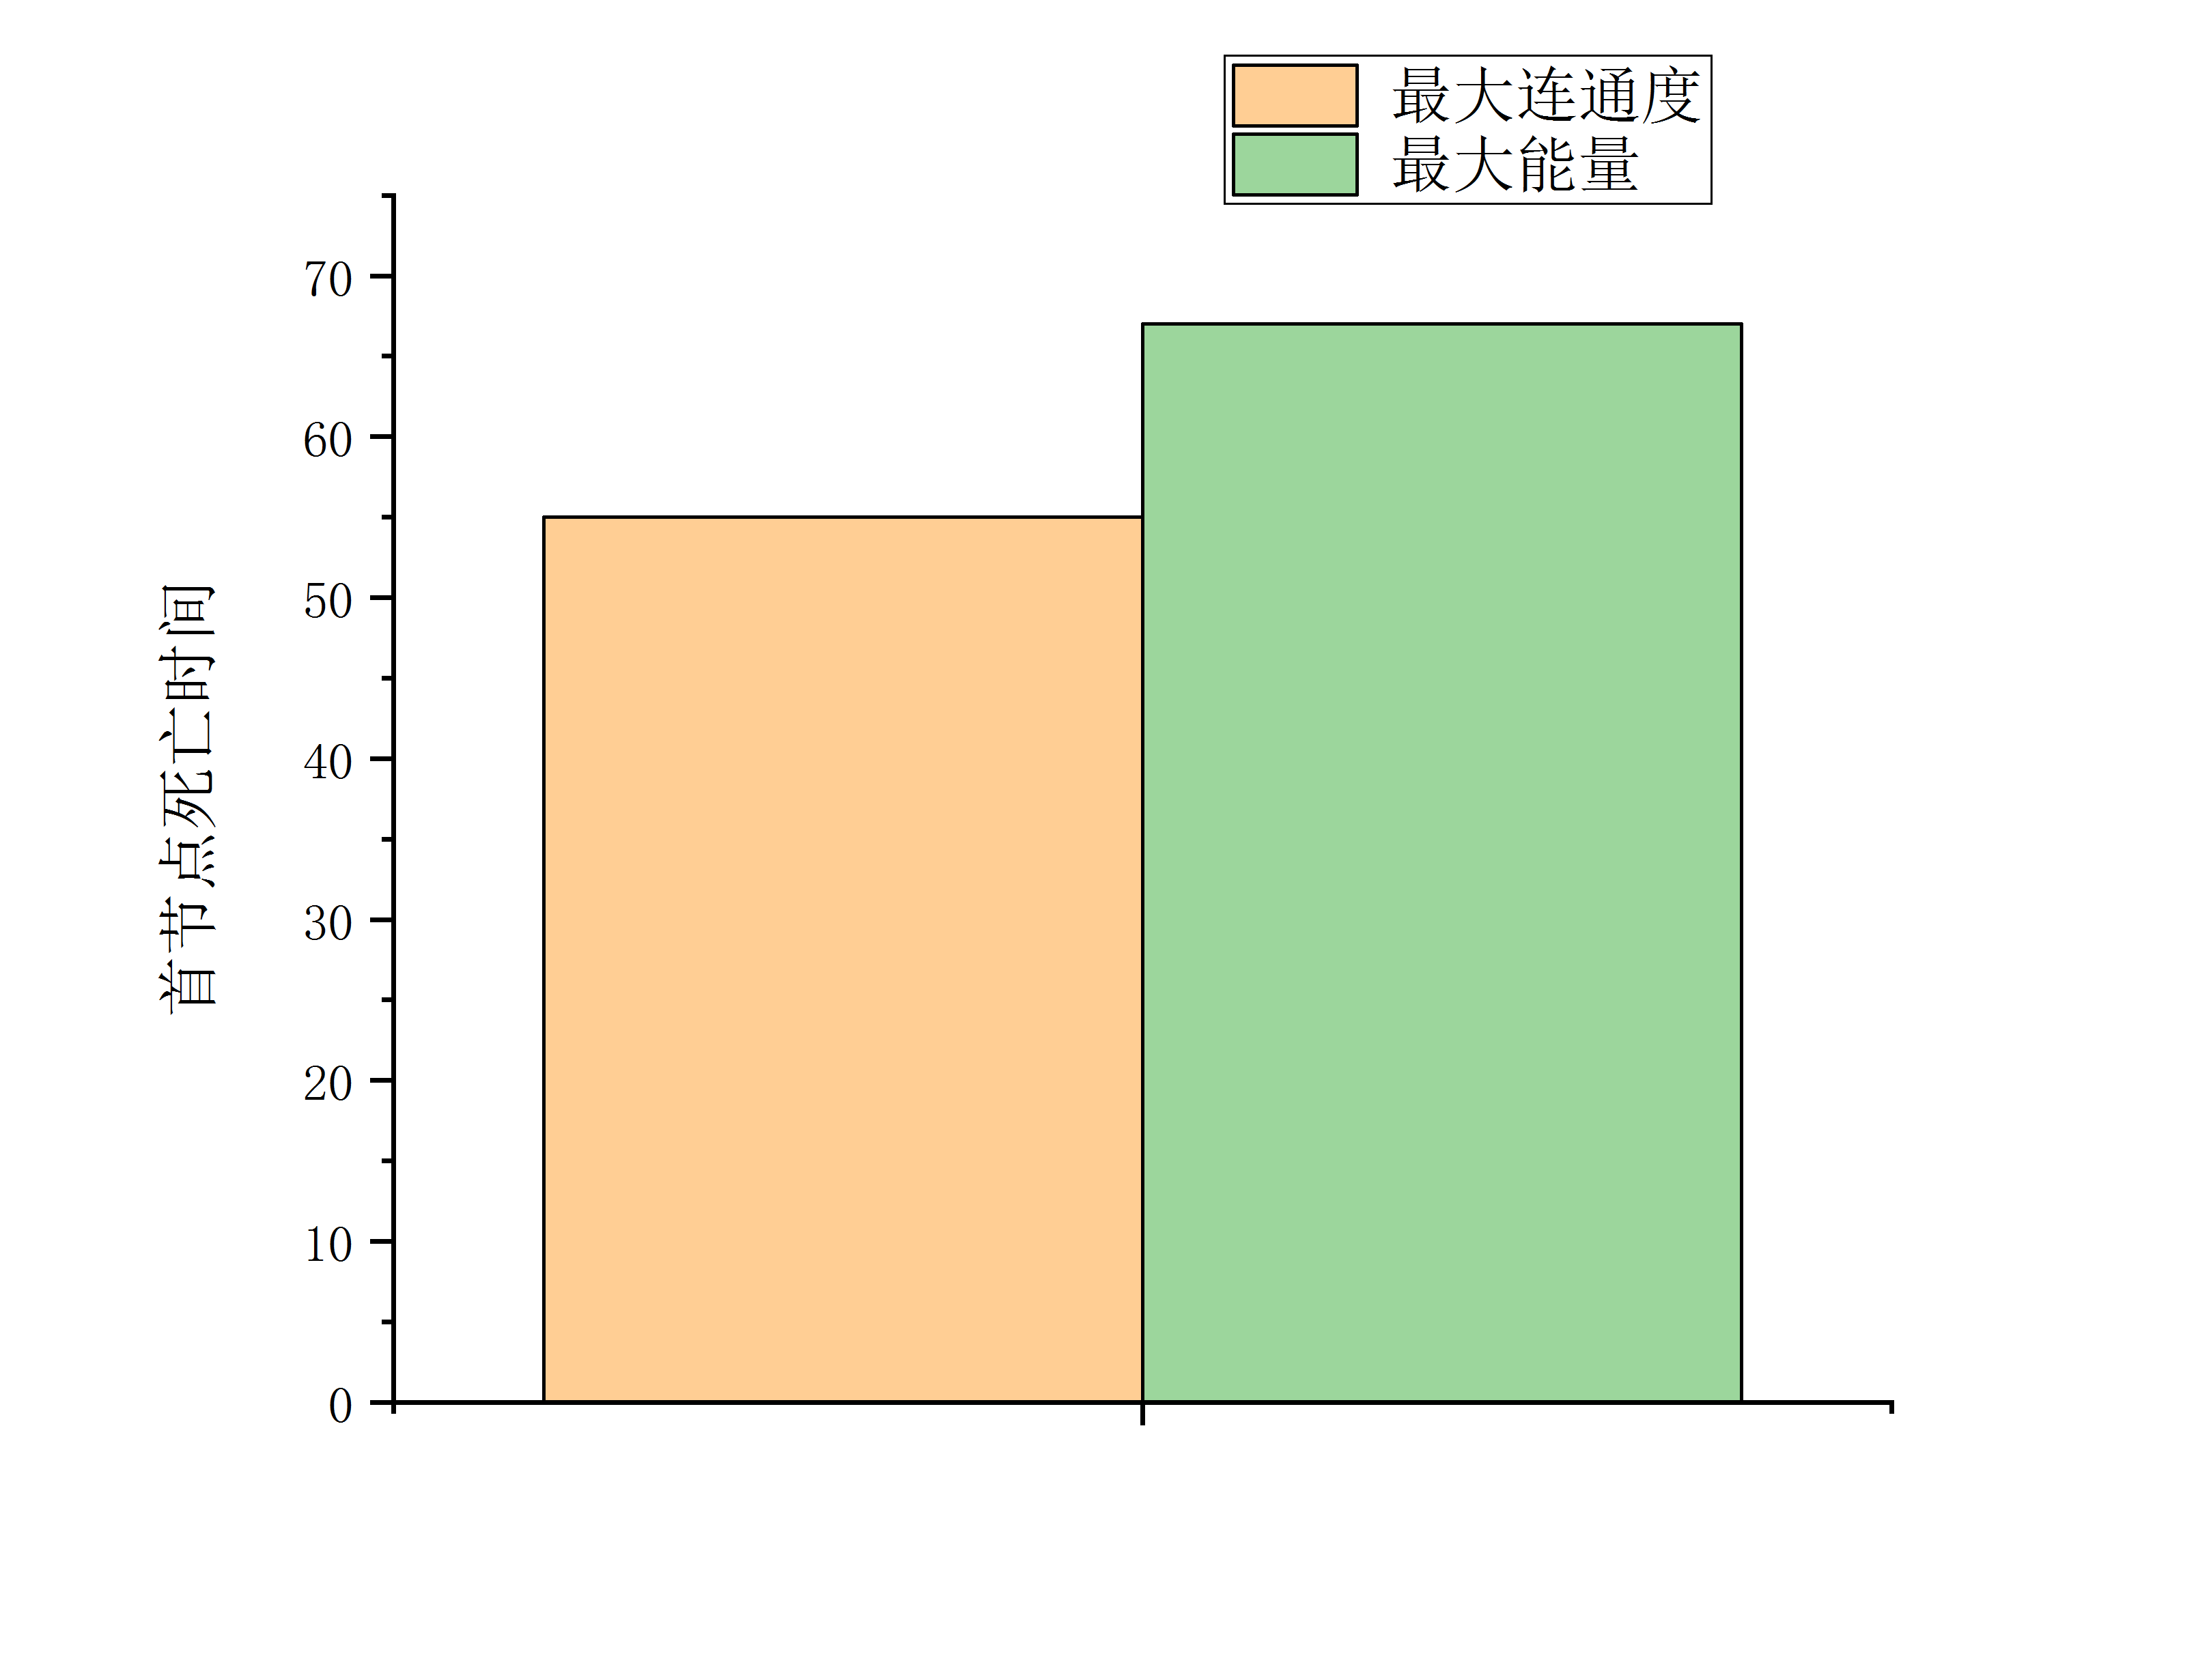
\includegraphics[scale=0.3]{pictures/siwang-routing.png} 
\caption{首节点死亡时间对比 } %插入图片的标题,一般放在图片的下方,放在表格的上方
\label{siwang-routing}
\end{figure}
 \begin{figure}[htbp]
\centering %使插入的图片居中显示
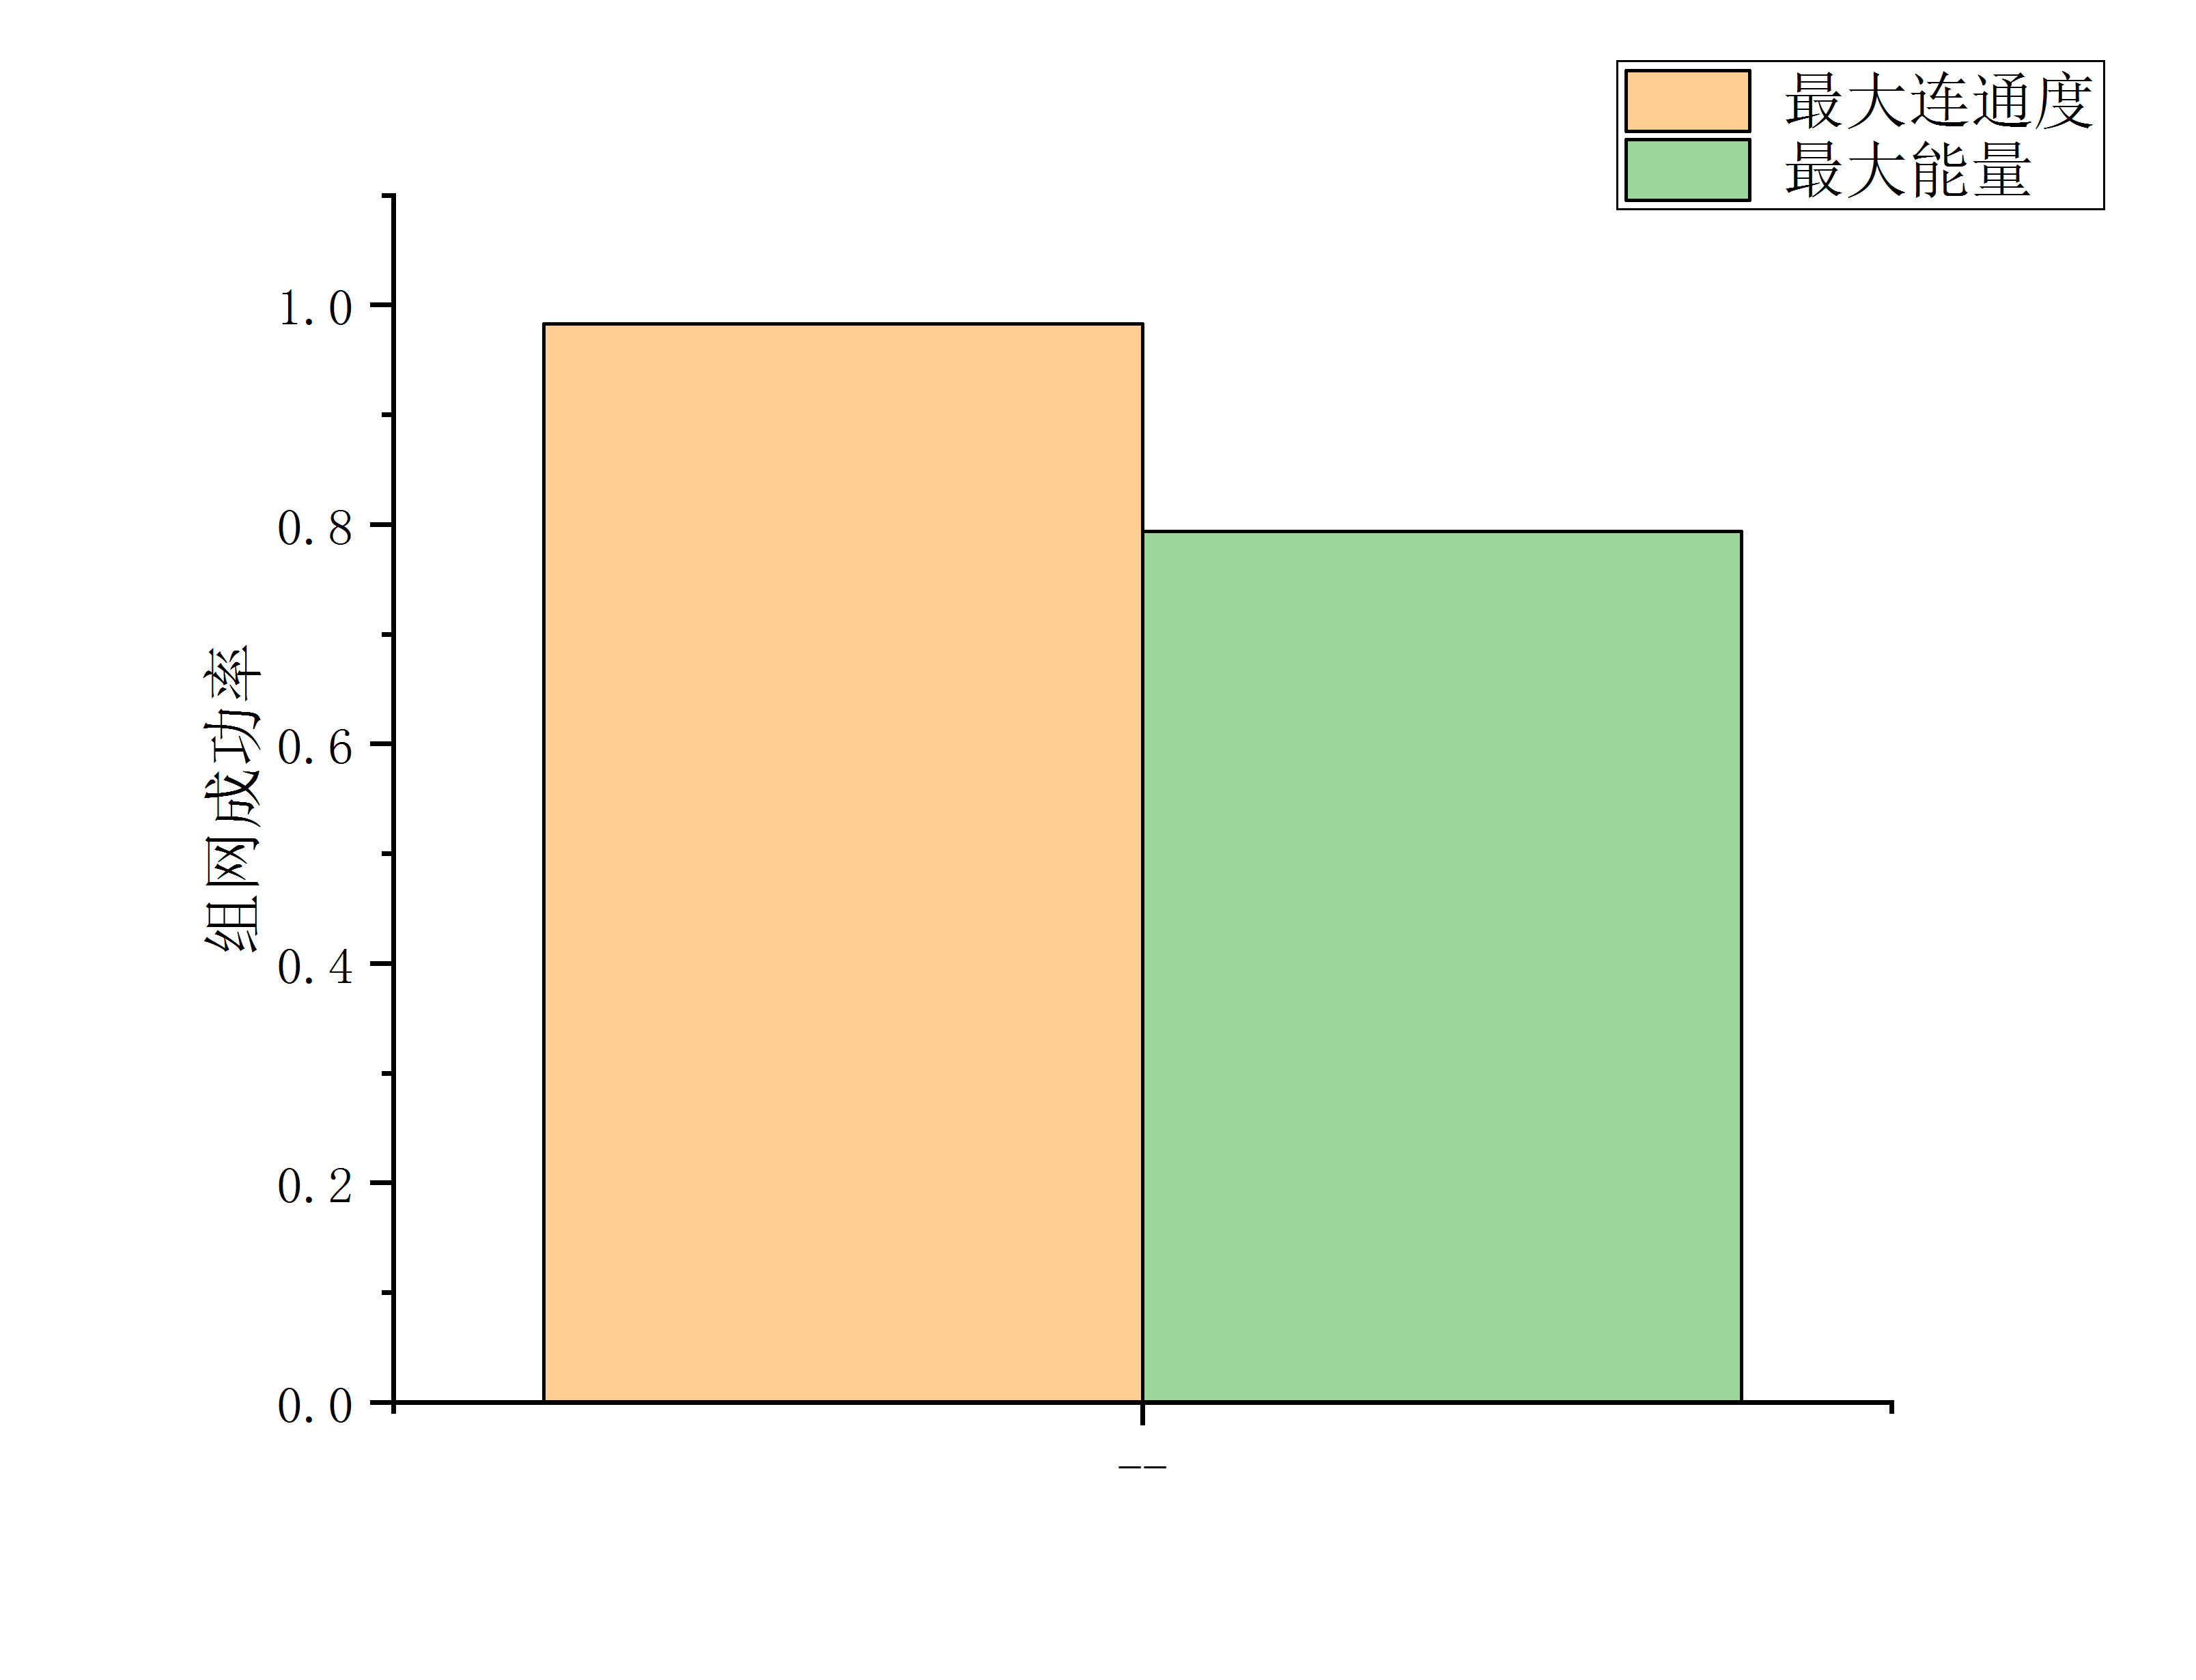
\includegraphics[scale=0.3]{pictures/routing-success.png} 
\caption{组网成功率对比 } %插入图片的标题,一般放在图片的下方,放在表格的上方
\label{routing-success}
\end{figure}
  \chapter{总结与展望}
\section{论文总结}
  本文给出了认识无线电组网的一种策略,方案中包括了从节点交汇到路由发现和数据传输的整个阶段,第二章中详细地对算法的执行过程进行了描述,并在第三章中给出了仿真结果与分析,并尝试了一种改进策略。
 \section{论文展望}
  上文中模拟了从节点交会到正常通信的全过程,但是文章的缺点也是显而易见的,成簇的算法作为一种分布式与集中式两者的妥协产生的结果,在获得了两者的部分优点的条件下,也同样具备了两者的缺点,簇头作为网络中权值较重的节点,担任着本不应该由普通节点担任的责任,这样实际上破坏了节点间的公平性,所以若是想要解决这个问题,需要提出一种周期性簇头轮换策略,但是又应该保证轮换过程中簇结构不会发生较大改变,避免对正常通信产生过大的干扰,这需要一个能量与连通性之间的权值,综合考虑两种因素之后决定应该由那个节点担当簇头,另外一种策略就是抛弃分簇思想直接从分布式结构入手,这样符合了节点间的公平性,但是也不再拥有低难度的设计参考,对系统方案的设计者提出了更高的要求,因为既要满足节点的自私策略又要获得最佳的通信效果与网络寿命。
%%%%%%%%%%%%%%%%%%%%%%% Main Area ENDs Here %%%%%%%%%%%%%%%%%%%%%%%%
%\let\cleardoublepage=\cleardoublepagebak
% Reference
\clearpage\phantomsection\addcontentsline{toc}{chapter}{参考文献}
\bibliographystyle{buptbachelor}
\refbodyfont{\bibliography{ref}}

% Thanks to page
\clearpage\phantomsection\addcontentsline{toc}{chapter}{致\qquad{}谢}
\chapter*{致\qquad{}谢}
  normalize
% Appendix

\newpage\backmatter
% Translation
\chapter*{外\quad{}文\quad{}译\quad{}文}
\vspace{8mm}

\thispagestyle{empty}

\begin{center}
\sihao\heiti{多跳多无线电认知网络中频谱切换调度与路由的联合优化}

\xiaosihao\songti{Mustafa Ozger, Fatih Alagoz, and Ozgur B. Akan }

\xiaosihao\songti{IEEE Communications Magazine}
\end{center}

\songti{}
\chapter{摘要}
  认知无线电可以动态频谱访问在空闲时使用许可的频谱。CR技术被应用于无线自组网和传感器网络中,分别形成了CRAHNs和CRSNs。簇是一种高效的拓扑管理技术,通过对CRAHNs和CRSNs中节点的认知能力来规范通信和分配频谱资源。在本文中,我们将深入研究这些网络中的拓扑、频谱和能量管理等簇的优点和功能。我们还概述了在CRAHNs和CRSNs中成簇的原因和挑战。对现有的成簇方案进行了回顾和比较。最后,我们揭示了在多通道CRAHNs和CRSNs中对频谱感知的主要想法和可能的解决方案。
\chapter{前言}
  对无线通信的过度需求导致了频谱短缺,虽然没有授权的频谱频带过于拥挤,但许可的频段并没有得到有效利用。认知无线电(CR)是一种很有希望的解决方案,它可以通过使二级用户(SUs)的动态频谱访问(DSA)机会性使用空闲的许可频带。因此,CR通过访问许可的通道,而无需对授权用户进行任何干扰,从而保证主用户的通信。
  
  在无线网络中,认知用户与主用户共存,这种网络被命名为认知网络。如图1所示,它们可以被划分为四个不同维度的区域。首先,这样的网络可以利用单一的许可频段或多个授权信道。第二,这个网络可能有一个集中式的或分布式的网络架构。集中式的无线网络,即认知无线电网络(CRNs),用基站来管理无线通信。另一方面,在分布式系统中,有一个没有任何中央实体来规范二次通信的扁平架构。这些分布式的支持cr的无线网络可以被称为认知无线电特别和传感器网络。认知无线电自组网(CRAHNs)是由CR技术支持的平面架构,以充分利用稀缺的许可频谱[1]。与CRAHNs不同的是,认知无线电传感器网络(CRSNs)被用于感知,并由具有更低计算能力和有限电池电量的节点组成[2]。这篇文章主要内容是关于多通道CRAHNs和CRSNs的领域,如图1所示。每一个SU都有DSA功能,即频谱感应来决定空闲的许可信道,频谱决策来决定操作通道,以及频谱切换,以在主用户到达时清空操作中的信道,因此,SUs使用这些功能来发现频谱空穴,即不在占用的空的许可频段。SUs与PUs共存,它们都被随机部署在网络中。因此,主用户的活动引起了附近SUs的频谱空穴的时间变化。另一方面,阴影、衰落和网络拓扑是导致空闲频谱带的变化的主要因素,阴影和衰落影响频谱感知,以及造成错误警报和错误检测的主用户活动都会对认知用户产生影响。网络拓扑根据认知用户的相对传输范围的不同而有所不同。对于CRAHNs和CRSNs,有两种网络拓扑结构[3]。在拓扑I中,在不同授权的通道中运行的网络中有一些主用户,然而,主用户网络的传输范围比认知网络大,因此主用户网络覆盖了一个辅助网络(r>>R),如图2a所示。根据授权频带内主用户的活动,将会产生时间变化的频谱空穴。此外,由于阴影和衰落的影响,空闲频谱也会有空间变化。因此,在可使用的授权频段的认知设备会出现时空变化,尽管图2a中使用通道1和2的两个主用户覆盖了所有的CRs,其范围内的认知设备的空通道列表可能仍然会有所不同。
  
  在拓扑II中,主用户的传输范围可以与认知设备(R>r)的传输范围相比,如图2b所示。因此,即使所有的主用户都使用他们的许可频谱,对于位于传输范围之外的认知节点也会有频谱空穴可以使用。此外,在信道使用中,时间的变化导致了在其传输范围内的认知设备的频谱可用性的时间变化。这个模型产生了一个非常动态的无线电环境。提出的网络解决方案必须考虑在多通道的CRAHNs和CRSNs之间的协调。成簇是一种基本的解决方案,可用于管理分布式无线网络中的通信[4]。这种方法可以在逻辑上对节点分组,每个这种组都被称为一个簇。在簇结构中,有一个簇头,它组织簇内成员之间的通信和簇间通信。因此,分布式网络通过簇头的成簇来提高网络中的通信性能,从而实现稳定和协作[4]。由于拓扑I和拓扑II的PU活动,在这个高度动态的无线电环境中,CRAHNs和CRSNs也受益于簇来协调频谱感知的结果。因此,成簇需要考虑簇内成员CRAHNs和CRSNs之间常见的空闲许可信道,以及簇头和簇内成员的地理位置。因此,这种类型的簇被称为频谱感知簇。由于该特性,成簇被作为一种功能工具,用于认知周期功能、访问控制、路由和管理多通道通信。尽管有其优势,但必须仔细考虑一些关键的挑战,例如异构的授权渠道和网络中空闲信道的动态变化,在此基础上提出成簇解决方案。本文组织如下。下一节将详细解释簇的功能。在此之后,我们讲解成簇过程并解释其中的挑战。在此基础上,提出现有的聚类方案,并在此基础上对现有的聚类方案进行了比较。接下来,我们提出了对CRAHNs和CRSNs的设计考虑和一种很有潜力的成簇解决方案。最后一节总结我们的文章。
 \chapter{簇在CRAHNs和CRSNs中的功能}
  本节详细阐述了簇如何应用于各种功能及其与网络操作的通信。这些功能广泛涉及三个操作领域,即感知、网络层和DSA操作,如图3所示。每个操作区域的详细解释在下面的小节中给出。
  
\begin{center}
\textbf{感知操作}
\end{center}

  传感器网络利用簇,利用相关性对簇头聚集的信息进行分类,因此,簇可以利用传感器节点对频谱感知的空间和时间相关性。由于观测与时间和空间域相关,所以这两种拓扑都能从簇中受益。簇的另一个好处是由于成簇而减少的数据包传输,因此减少了能源消耗。由于聚合的原因,感知相关性会影响路由、中间访问和无线传输功能。
  
  \begin{center}
\textbf{网络层操作}
\end{center}

  簇为无线自组织网络中提供了路由功能。然而,由于可用频段的动态变化,认知网络带来了额外的挑战,即通信的认知设备之间的一个公共通道是转发数据包的一个附加条件,也是束缚通信的一个因素。由于簇的形成依赖于利用空间和时间相关形成的成员之间的公共信道,所以为源节点与目的节点之间的通信减小路由路由开销提出了新的要求。因此,两种网络拓扑都可以利用簇的路由功能。参考文献[5,6]是两个例子,解释了如何在动态的无线电环境中使用簇来进行路由发现。文献[5]中提出了从单独事件到事件槽的成簇方案。根据DSA和服务质量(QoS)要求,簇也被用于在CRSNs中为多媒体数据包提供路由[6]。

  簇也提供了中间访问的功能,在动态无线电环境中,最重要的因素之一是空闲许可信道的PU的存在和争用问题。可以设计一个中等访问方案,这样簇中的每个节点都可以访问空闲通道[7]。基于簇的介质访问提供了更高的吞吐量和更小的延迟和更少的能源消耗。簇头可以作为协调器,在感知空通道协作后,作为访问频谱的协调器。在两种拓扑中都可以使用簇来进行介质访问,以支持基于许可频带的空间和时间变化的频谱感知通信。

\begin{center}
\textbf{动态频谱介入操作}
\end{center}

  频谱共享和决策操作是服务于特定目标的。争夺空置的授权频段和PU的出现是共享频谱和决定一个通信用的波段的两个重要因素。由于簇是根据常见的空信道形成的,簇头决定簇内通信的操作通信通道,这有助于频谱决策。例如,可以利用成簇来减少功率和子通道分配对SU的干扰[8]。成簇在频谱共享与频谱决策两个方面对两种拓扑都是有益的。频谱感知是DSA的一项操作。簇内的节点将会把各自的频谱感知结果发送给簇头,簇头将会进行空白授权频段的本地频谱决策。簇头将会决策PU的存在性,从而会对物理层产生影响,簇内的节点通过协作来达到频谱感知结果的共识,虽然成簇可以用于两种拓扑结构,但是主要用于拓扑1中,这是因为拓扑1中的空间变化较少,由于频谱感知的阴影,衰落和感知结果的不完整性,簇内的节点需要通过合作来确定拓扑中频带的空缺。

  在整个网络中,CRAHNs和CRSNs的另一个问题是公共控制通道的可用性。簇功能提供了簇内成员之间的本地控制通道,簇内成员之间的控制消息通过这些控制通道传输[9]。由于拓扑II引起高度动态的空间和时间变化,控制信道分配更适合拓扑II。


\begin{center}
\textbf{CRAHNs与CRSNs中的成簇动机与挑战}
\end{center}

  成簇是一种组织整个网络的十分有效的方法,并且可以作为本地的协调器,以便能够以结构化的方式执行频谱感知结果的通信,因此我们详细描述了这两种网络中的关键过程与挑战。


\begin{center}
\textbf{成簇动机}
\end{center}

  成簇可以形成逻辑组,以便更好地利用特定网络中的资源。它对DSA的自组网更有好处,因为可以通过将邻居节点按其空闲信道分组来高效地执行频谱感知通信。因此,我们详细列出了成簇的动机。

  节点间的协调:在每个集群中,有一个集群头控制其组内的通信。此外,相邻的簇头可以通过它们的公共通道直接通信,也可以通过它们的成员通过多个跃点进行通信。簇头可以被认为是调节SUs之间的频谱感知通信的虚拟通道,它使得SU之间实现协调。

 可伸缩性:Ad hoc和传感器网络具有较高的网络密度,因此这些网络中的协议和解决方案可能无法扩展。在已经提出的方案中,网络的可伸缩性会由于认知节点在频谱的高度动态变化环境中不断进行通信而产生变化,在同构网络之上,簇可以产生虚拟节点(即:为了提高网络的可扩展性[4]。

  网络性能的改进:在多通道动态无线电环境中,相邻节点按其空闲许可信道进行分组。如果簇中的一个公共通道被PU占用,簇内的通信将继续通过另一个公共通道进行。因此,由于具有频谱感知的聚合,CRAHNs和CRSNs在其操作通道上可以对PU到达者免疫,从而提高了网络性能。

  节点间的协作:认知周期循环,即频谱感知、频谱决策和频谱切换,可以以一种高度结构化的方式进行聚类管理。这些复杂的任务以集群成员之间的协作方式执行。由于簇内成员之间有共同的通道,簇头可以很容易地协助合作。此外,簇头之间的协作可以提高节点的通信性能。

  建立局部控制通道:在频谱感知通信中最重要的问题是在整个网络中假设一个公共控制信道。然而,由于整个网络中空闲的许可信道的动态行为(例如,主用户的活动),这种假设是无法实现的。由于簇是在一个社区内形成的,所以簇中存在着用于调节簇内成员间通信的本地公共控制通道。

  多通道通信支持:每个簇内成员之间有多个公共通道,因此,簇头可以通过同时支持多个信道的使用,在簇成员之间分配频谱资源。

\begin{center}
\textbf{成簇的挑战}
\end{center}

  除了成簇动机中提出的要求,CRAHNs和CRSNs同样也有着不同的挑战,具体内容如下。

  多信道的环境:认知功能CR提供PU占用的信道的利用率。在这种类型的环境中,成簇是根据物理接近性和节点形成簇之间的共同通道来进行的。因此,节点应该知道空闲的许可信道,同时整个簇需要调优到同一频段进行通信。

  许可频带可用性的动态变化:威胁集群稳定性的最重要因素之一是集群中空白频段的动态变化。如果集群成员之间没有公共通道,则应该重新聚集这些节点。因此,形成的网络必须对可用谱带的变化具有很强的鲁棒性。此外,频繁的重新聚类会导致新簇形成的控制信息导致能量消耗。

  许可信道的异质性:在多通道CRSNs和CRAHNs中,许可信道的特性(如带宽和载波频率)可能存在不同。这种差异可能导致不同的比特率、传输范围等。

\begin{center}
\textbf{Spectrum-Aware集群方案}
\end{center}

  在集群成员中拥有常见的空闲授权信道是文献中对频谱感知聚类协议的共同要求。然而,在形成集群的同时,它们在邻近区域有不同的方法。我们概述了最近在动态无线电环境中成簇的现有方法。

  鲁棒谱共享(ROSS)[10]:这种聚类方案的目标是簇的鲁棒性,这意味着在增加PU活动的情况下,簇的最终可持续性。[10]的作者提出了一种分布式聚类算法,该算法能够通过CR节点的相邻节点之间的相互作用来实现簇的形成。它包括两个级联阶段,即簇形成和成员资格的确认。首先,根据连接性向量来选择簇头,它由个体连接度和邻域连接性程度组成。在此阶段,保证簇成员之间的公共通道,并控制簇大小。在此之后是簇内成员资格的确认。簇内成员资格的确认过程被视为一种拥塞游戏。有争议的节点大多是不同集群的重叠节点,在加入不同的簇之后,应当选择具有最高公共通道的簇加入。

  关联传播(AP)[11]:该算法应用亲和传播,使CR节点作为数据点,簇头作为样本。其主要目的是减少整个网络中簇的数量,相似性度量的是CRs共享的公共通道,簇的目标是尽可能多地使用簇中其他节点的可用通道,而选择作为簇头的概率是由CRs的节点度决定的。

  频谱机会成簇(SOC) [9]: SOC是一种成簇算法。簇的形成有三个步骤。在第一步中,节点知道它们的邻居和它们的空通道,它们形成了邻居表,表包括最大可用性边与最大度数的节点信息,这些表将会向所有邻居广播,第二步中将会根据最大的簇或者最多度数的边选择最佳表,那些包含在多个簇中的节点会被移除,簇头则是与簇内成员只有单跳距离的节点,这也是第三部的操作。

  组合[12]:在这种成簇方案中,节点知道它们的k跳邻居及其对应的空通道,所有的CRs都计算与k跳邻居的最小公共通道数。根据这一信息,每个CR都分配一个权重,用于簇头的选择过程。其邻域内权重最高的节点成为簇头。这些节点向集群发送成员请求。如果一个节点收到多个请求,它将选择权重最高的一个。

  CogLEACH[13]:在这种成簇方法中,簇头的期望数目是固定的,并且通道数量较多的节点更有可能成为簇头。根据这些条件,每个节点都被分配一个成为簇头的概率。非簇头节点根据接收到的信号强度将连接请求发送到簇头,并以最少的通信成本发送连接请求。

  分布式频谱感知聚类(DSAC) [14]: DSAC方案试图将总能耗最小化,这是簇内和簇间通信消耗的能量之和。根据平均消耗能量确定了最优簇数。对于分布式算法,将可用通道约束局部最接近的对合并为簇。

  表1总结了上述讨论,并根据网络对现有的成簇方案进行了总体比较,并给出了成簇的步骤。

\begin{center}
\textbf{CRAHNs与CRSNs的分布式成簇}
\end{center}

  尽管在文献中存在频谱管理、介质访问控制和路由解决方案的成簇方案,但没有足够的成簇方案研究来满足CRAHNs和CRSNs的内在要求。为此,我们确定了网络需求和簇设计两者作为考虑因素。之后,我们简要概述了在CRAHNs中分布式集群方法的潜在解决方案,以及在CRSNs中的事件驱动成簇方法。

\begin{center}
\textbf{网络需求}
\end{center}
  CRAHNs有独特的需求,其中之一是由于认知设备与主用户的流动性,管理频谱利用率的高变化频率。此外,必须满足不同的QoS需求。例如,多媒体应用程序需要有限的延迟和较低的抖动。另一个要求是对主用户的干扰是有限的。如果是因为主用户活动影响到信道,那么这将会干扰主用户活动,这是不可取的。
  在CRSNs中有更多的对于簇的需求。首先,传感器节点的电池电量有限。因此,成簇解决方案必须是节能的。由于成簇需要一个控制信道进行控制与维护,我们提出的解决方案必须防止出现过大的开销,因为过大的开销将会提高认知设备的能耗水平。在认知操作方面,提出的簇应避免操作通道的频繁变化,因为频谱切换和频谱感知等认知周期功能消耗了大量的能量。此外,传感器节点的计算能量有限。因此,建议的聚类方法应该很简单。能量效率和低计算开销是CRSNs中成簇解决方案的两个额外要求。

\begin{center}
\textbf{成簇设计考虑事项}
\end{center}

  CR设备的操作与网络架构是在设计网络架构中主要需要考虑的因素。由于认知自组网与认知传感网络的不同要求,成簇的注意事项也会有所不同。因此我们解释了这两种网络中的相同与不同之处。
  
  常见的设计考虑:第一个共同的考虑是,在形成的集群中至少需要有一个相互的空通道。簇节点必须通过公共通道进行通信。

  频谱感知的缺陷也很重要,因为成簇是根据空谱带进行的。由于信道感知性能较差,可以根据CRs的错误空通道列表来形成簇。由于其简单性[1],常用的频谱感知方法是能量检测[0]。然而,这种方法在传感过程中存在缺陷。因此,误检和误报的概率对于簇的稳定性是很重要的。

  节点的移动性极大地影响了频谱利用率的异质性,这直接改变了簇的形成。由于SU的移动性,簇头可能失去与成员的连接。因此,应该为集群中的传入和传出节点设计簇结构更改、关联和分离机制。此外,主用户的移动性会使SU的频谱利用率发生更动态的时空变化。

  对簇的维护是另一个考虑因素。高度变化的授权用户活动增加了维护簇的成本。由于这些动态影响,一些节点可能会离开当前的簇,或者加入另一个节点,从而导致包开销和能源消耗。

  针对CRAHNs的设计考虑:在特定网络中的流有不同的QoS级别。由于主用户的活动,这种考虑变得困难。簇必须考虑到它们来支持不同的QoS级别。为了支持更好的通信质量,簇的另一个考虑是异构的许可信道,这导致了不同的特性,如传输范围和比特率。在集束形成过程中,必须利用较少的PU到达通道来降低频谱切换的概率,当然这也会增加能量消耗。

  特定于CRSNs的设计考虑:CRSNs是具有事件驱动的通信。节点在发现事件后报告其观察结果。如果频率足够低,那么在事件发生后就不需要维护集群,因为在下一次事件之前它们不会被使用。集群解决方案应该考虑CRSNs的这种独特属性。

  能源效率是CRSNs的另一个考虑因素,因为节点的电力有限。尽管簇提供了能量节省策略,但由于重新聚类和控制开销,认知用户活动可能会降低集群所提供的能源效率。

\begin{center}
\textbf{对CRAHNs的分布式集群方法}
\end{center}

  在CRAHNs中没有一个集中的实体需要CR之间的合作。簇提供了自组网结构之上的层次结构,以改善网络中的本地合作。为此,我们解释了分布式成簇方法中可能存在的问题和解决方案。

  在整个网络中存在一个共同控制信道的普遍假设。但是,由于PU的活动,这是很不现实的。为了使它更真实,这个通道被认为是一个非常窄带的通道,它可能容易堵塞。因此,提出的协议不能依赖于这样一个通道的存在。可以通过通道跳跃或会合方法通过相同的通道进行通信,以配合小区内簇的形成。但是,由于通道切换,这种方法有很高的开销。针对分布式认知无线电网络,提出了一种盲交会算法,使通信节点不需要一个通用的控制信道和可用的信道信息[15]。该算法保证在不需要时间同步的情况下进行集合,并占用较短的时间进行成簇。

  现有的集群方案形成了针对动态可用信道变化的健壮集群。因此,应该采用启发式算法来设计一种能够最大限度地增加簇中成员节点数目的聚类方案。可以建立公共通道大小和簇成员之间的平衡,以形成健壮的集群,如[9]。除了集群的形成之外,它们的维护是在现实场景中需要考虑的另一个问题。簇维护解决方案应该适应簇中公共通道的变化。簇头可以通过较少节点重新形成簇,以实现公共通道,相互连接的节点不应该减少公共信道的数量从而导致稳定性的降低。

  除了动态的无线电环境外,网络节点的移动性使得它们之间的合作更具挑战性。提出的成簇算法应该具有机动性。如果一个簇头与它的成员失去联系,这将导致重新聚类,这是一种高效的成簇方法应该避免的。为了解决这个问题,一个在其附近具有较高迁移率的节点不应该是簇头。节点可能有权重来度量节点的迁移率,以在本地社区中选择簇头。通过这样做,它不太可能重新聚合节点,因为簇头不会与它的成员断开连接。此外,簇必须管理传入和传出的认知设备,以更新簇成员来管理网络拓扑。簇中的无线电资源分配是由于移动节点的关联和分离而降低的。

  簇内的通信管理也应该考虑到频谱的流动性。簇的工作频带可能被占用;因此,簇内成员应该组织簇内的通信,从而使一个新的空通道具有有限的延迟。由于频谱切换,CR节点消耗能量。因此,应该选择最小PU到达统计量的集群通道作为操作通道,以避免频谱切换。根据PU的到达统计量来衡量通道,有助于选择更多的空闲通道进行簇内通信。

  现有的成簇方案假设有同质的许可信道,它们的信道特性是相同的。然而,在现实的多通道CRAHN场景中,它们的带宽和中心频率可能不同。因此,这些渠道的特点各不相同。例如,许可渠道的频谱感知结果在这种情况下是不同的。此外,授权渠道的比特率也不同。不同通道上的pu特性可能会有很大的差异,这就导致了变化频繁的通道可用性。如果网络需要更多的覆盖,形成集群的一个可能的解决方案是将相邻节点与具有较低中心频率的通道进行分组。
% Translated Article
\thispagestyle{empty}
\begin{center}
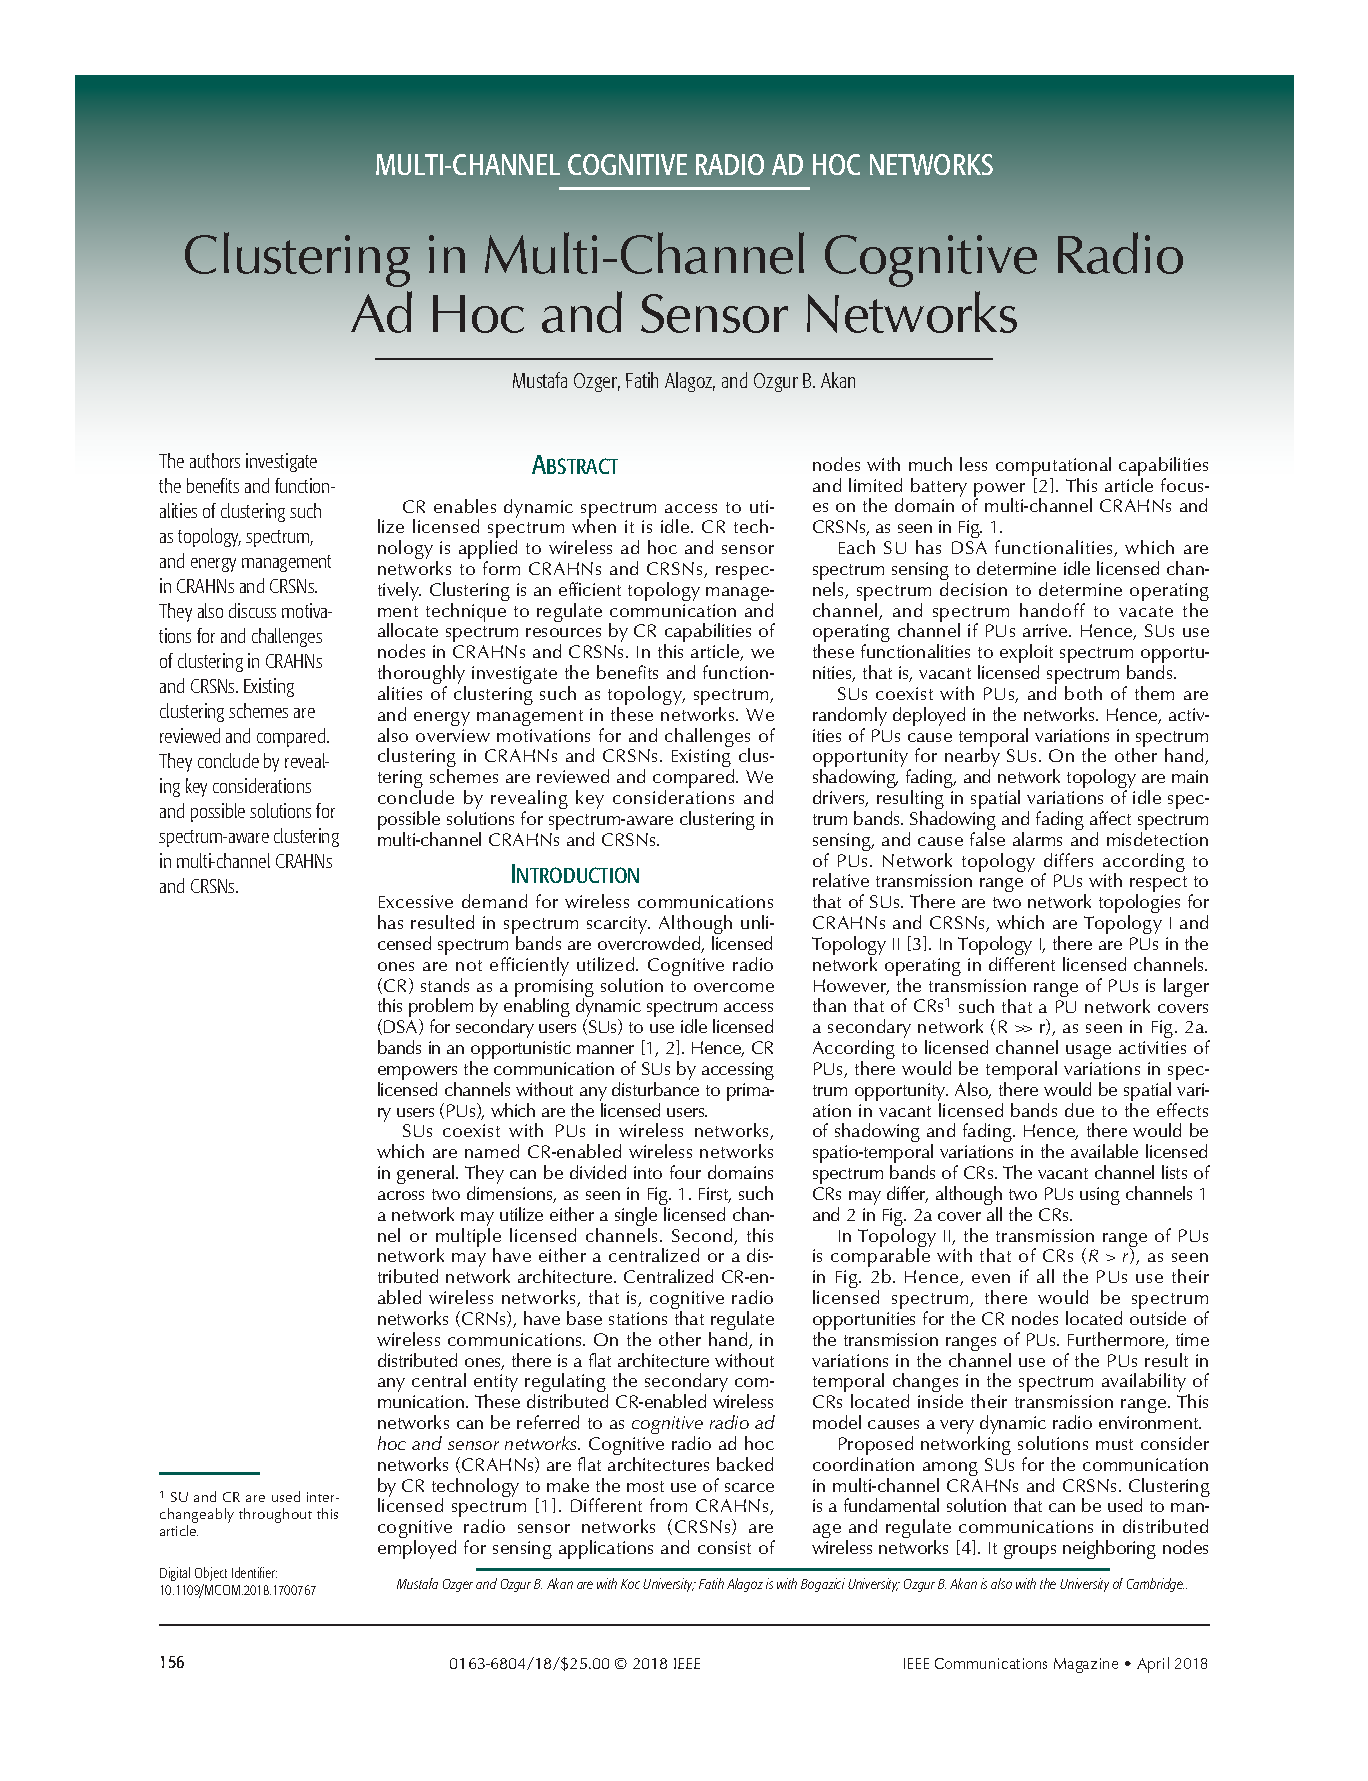
\includepdf[pages=1, scale=0.95, pagecommand=\heiti\sanhao{外\quad{}文\quad{}原\quad{}文}]{docs/translation.pdf}
\includepdf[pages=2-, scale=0.95, pagecommand={}]{docs/translation.pdf}
\end{center}

% 开题报告
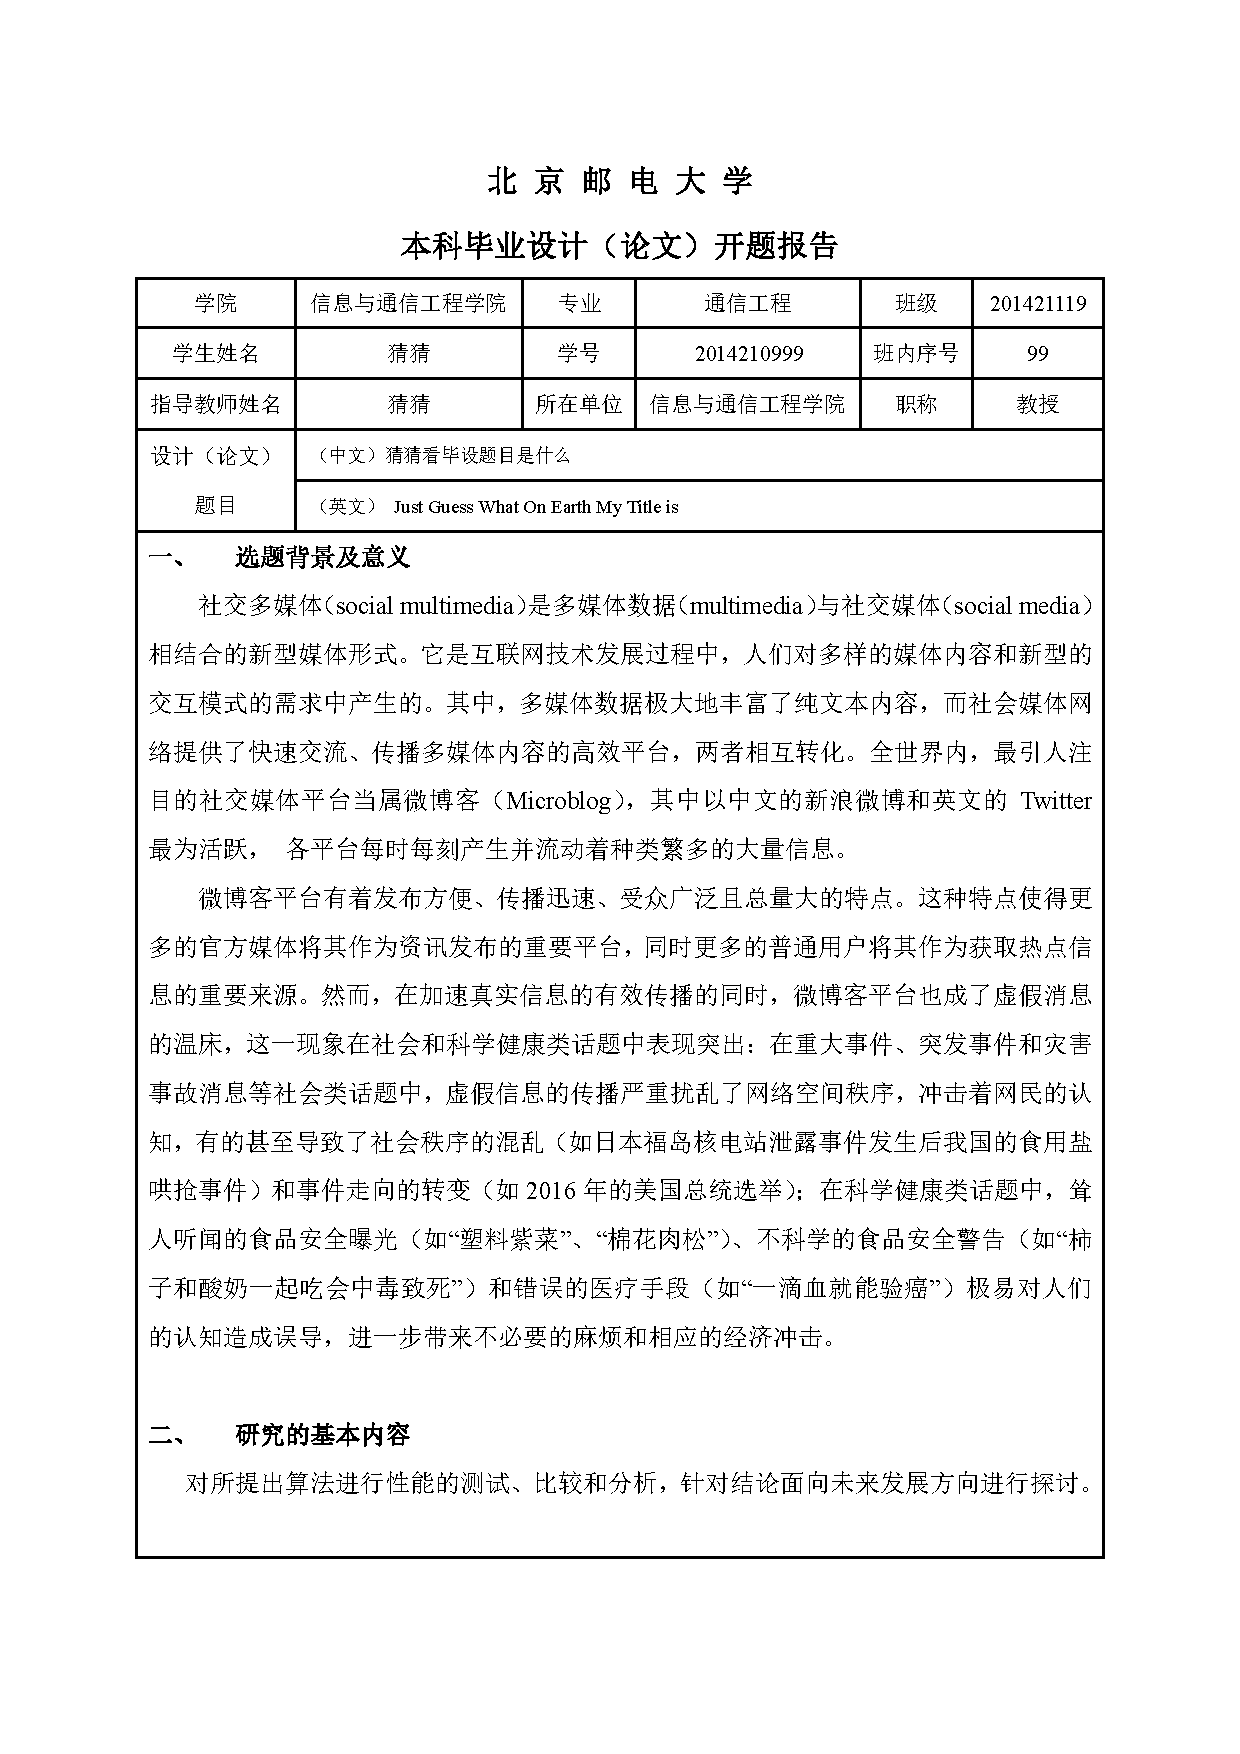
\includepdf[pages=-]{docs/openingReport.pdf} 


% 中期检查表
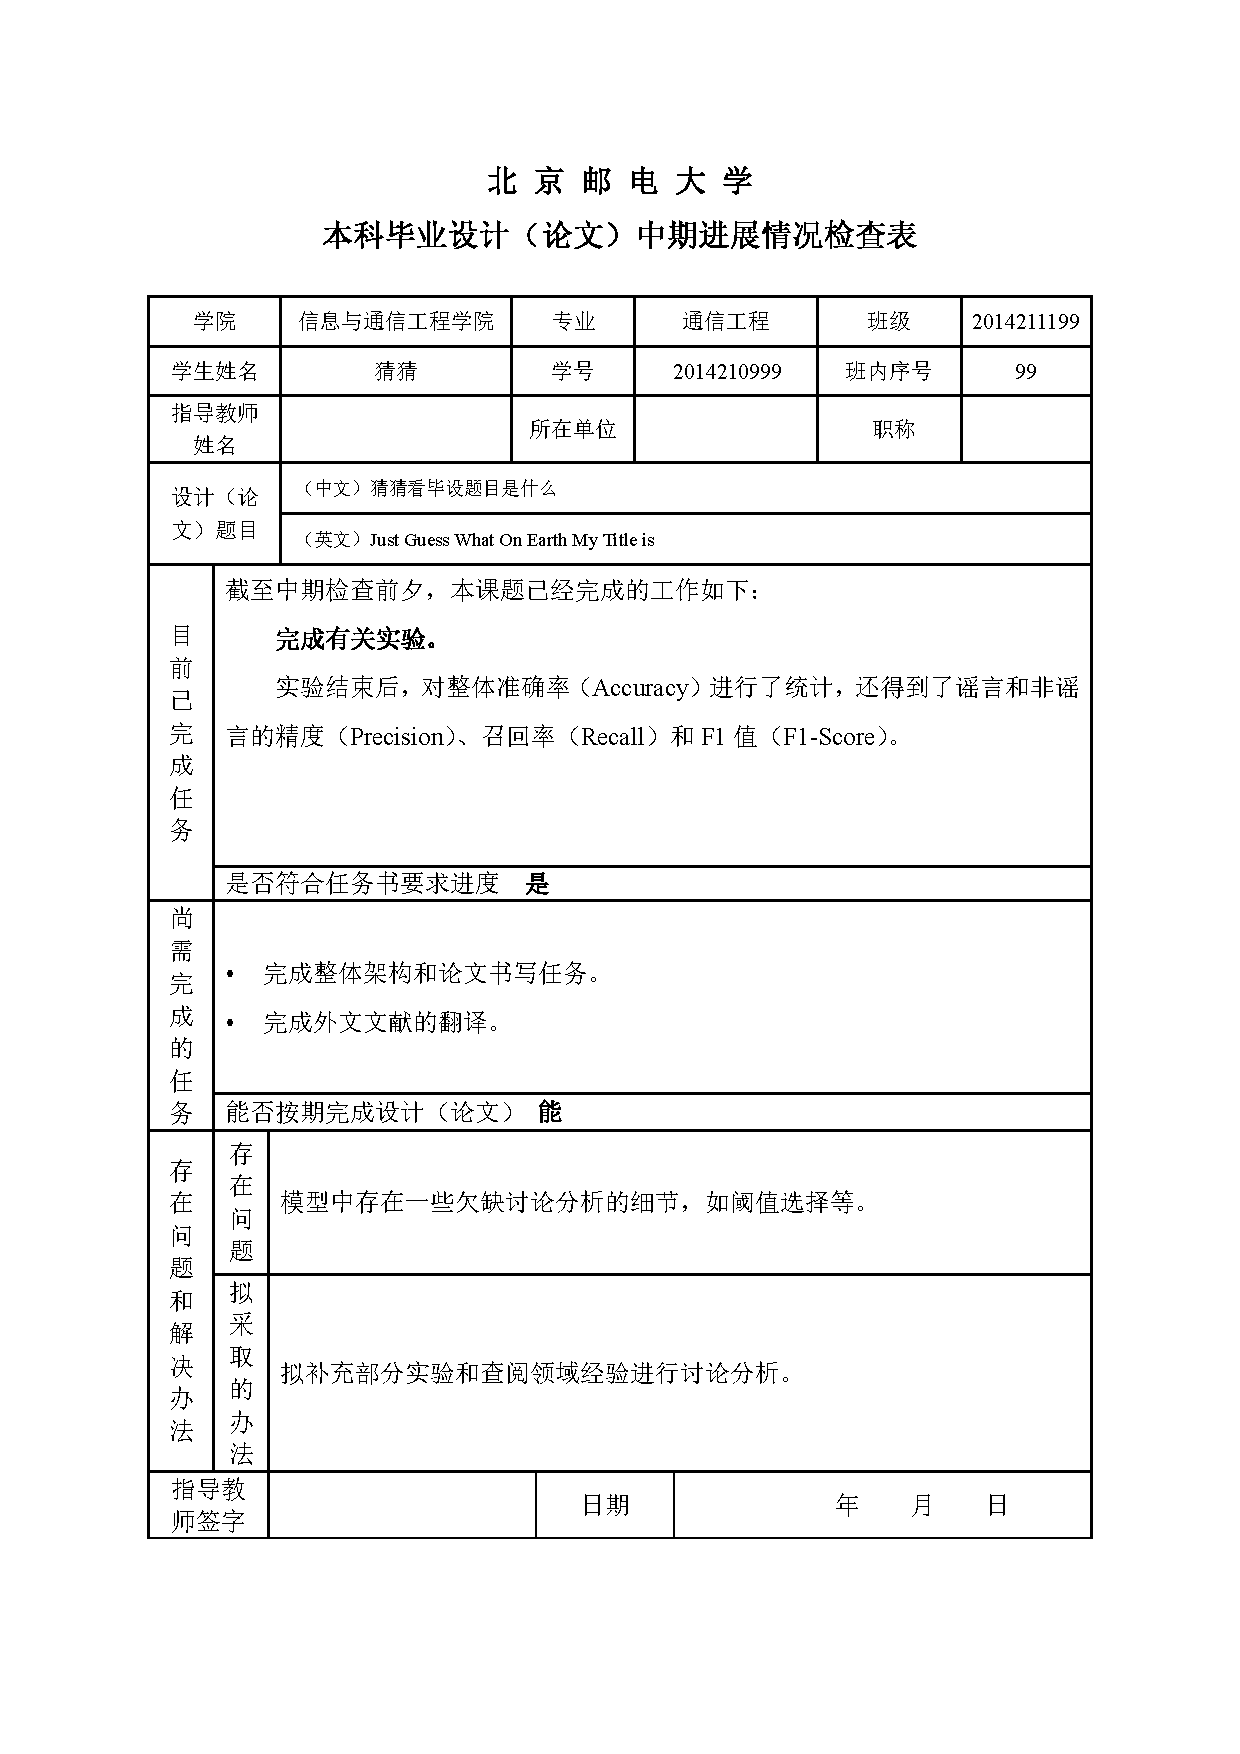
\includepdf[pages=-]{docs/interimReport.pdf} 


\end{document}
